% !TeX root = main.tex


%% newCommand
% voltages
\newcommand{\Ua}{U_{\mathrm{a}}}
\newcommand{\Ui}{U_{\mathrm{i}}}
\newcommand{\Uan}{U_{\mathrm{a,n}}}


% current
\newcommand{\Ia}{I_{\mathrm{a}}}
\newcommand{\In}{I_{\mathrm{n}}}

% resistor
\newcommand{\Ra}{R_{\mathrm{a}}}

% power
\newcommand{\Pn}{P_{\mathrm{n}}}
\newcommand{\Pl}{P_{\mathrm{l}}}
\newcommand{\Pfe}{P_{\mathrm{Fe}}}
\newcommand{\Pcu}{P_{\mathrm{Cu,a}}}

% torque
\newcommand{\Tn}{T_{\mathrm{n}}}

% speed
\newcommand{\nN}{n_{\mathrm{n}}}
\newcommand{\nO}{n_{\mathrm{0}}}

% flux
\newcommand{\phiDelta}{\phi_{\updelta}}

% machine design related parameter
\newcommand{\za}{z_{\mathrm{a}}}
\newcommand{\taup}{\tau_{\mathrm{p}}}
\newcommand{\lz}{l_{\mathrm{z}}}




%% add [solution]
\documentclass[solution]{../course_template/exerciseClass}
\title{Electrical Machines and Drives}

%%%%%%%%%%%%%%%%%%%%%%%%%%%%%%%%%%%%%%%%%%%%%%%%%%%%%%%%%%%%%%%%%%%%%%%%%%%%%
%%%Lecture Include Only%%%
%\includeonly{tex/exercise01, tex/exercise02, tex/exercise03}
%%%%%%%%%%%%%%%%%%%%%%%%%%%%%%%%%%%%%%%%%%%%%%%%%%%%%%%%%%%%%%%%%%%%%%%%%%%%%

\begin{document}

    %%%%%%%%%%%%%%%%%%%%%%%%%%%%%%%%%%%%%%%%%%%%%%%%%%%%%%%%%%%%%
%% Begin exercise %%
%%%%%%%%%%%%%%%%%%%%%%%%%%%%%%%%%%%%%%%%%%%%%%%%%%%%%%%%%%%%%
\ex{Semiconductor properties}


%%%%%%%%%%%%%%%%%%%%%%%%%%%%%%%%%%%%%%%%%%%%%%%%%%%%%%%%%%%%%
%% Task 1 %%
%%%%%%%%%%%%%%%%%%%%%%%%%%%%%%%%%%%%%%%%%%%%%%%%%%%%%%%%%%%%%

\task{Properties of germanium as semiconductor}

The following problems explore fundamental semiconductor properties of germanium. 
Starting with atomic concentration and intrinsic resistivity, the tasks gradually introduce doping effects 
and compare the electrical behavior of intrinsic and extrinsic materials under simplified assumptions. Take the values from \autoref{table:ex01_germanium_values}.

\begin{table}[ht]
    \centering  % Zentriert die Tabelle
    \begin{tabular}{ll}
        \toprule
        Intrinsic concentration $n_\mathrm{i}$: &  $\SI{10^{13}}{atoms\per{\cubic{\centi\meter}}}$\\ 
        Mobility $\mu_\mathrm{p}$: &  $\SI{1800}{\frac{\square{\centi\meter}}{\volt\second}}$ \\ 
        Mobility $\mu_\mathrm{n}$: &  $\SI{3800}{\frac{\square{\centi\meter}}{\volt\second}}$ \\ 
        Atomic weight $a_\mathrm{ger}$: &  $\SI{72.6}{\gram\per\mole}$ \\
        Material density $D_\mathrm{ger}$: &  $\SI{5.32}{\gram\per{\cubic{\centi\meter}}}$ \\ 
        \bottomrule
    \end{tabular}
    \caption{key figures of germanium at $\SI{300}{\kelvin}$.}  % Beschriftung der Tabelle
    \label{table:ex01_germanium_values}
\end{table}


\subtask{Using Avogadro’s number ($N_{Av}=\SI{6.02 \cdot 10{23}}{mol^{-1}}$), calculate the concentration of atoms in germanium.}

\begin{solutionblock}
    A quantity of any substance equal to its molecular weight in grams is a mole.
    So the concentration is calculated by
    \begin{equation}
        C_{Ger} = \frac{N_\mathrm{Av}}{a_\mathrm{ger}} \cdot D_\mathrm{ger}
        =\frac{\SI{6.02 \cdot 10{23}}{mol^{-1}}}{\SI{72.6}{\gram\per\mole}} \cdot \SI{5.32}{\gram\per{\cubic{\centi\meter}}}
        = \SI{4.41 \cdot 10^{22}}{atoms\per\mol}.
    \end{equation}
\end{solutionblock}

\subtask{Calculate the resistivity of intrinsic germanium at $\SI{300}{\kelvin}$.}

\begin{solutionblock}
    Using the equation $n=p=n_\mathrm{i}$ the conductivity of the intrinsic germanium is calculated by
    \begin{equation}
        \begin{aligned}
            \sigma  &= n_\mathrm{i}^2q(\mu_n+\mu_p) = \SI{2.5 \cdot 10^{13}}{atoms\per{\cubic{\centi\meter}}} \cdot \SI{1.60 \cdot 10^{-19}}{\coulomb}
            \cdot \left( \SI{3800}{\square{\centi\meter}\per{\volt\second}} + \SI{3800}{\square{\centi\meter}\per{\volt\second}} \right) \\
            &= \SI{0.00224}{\frac{1}{\ohm\centi\meter}}.
    \end{aligned}        
    \end{equation}
    The resistivity results by the reciprocal value:
    \begin{equation}
        \rho = \frac{1}{\sigma} = \frac{1}{\SI{0.00224}{1\per{\ohm\centi\meter}}}= \SI{44.6}{\ohm\centi\meter}.
    \end{equation}    
\end{solutionblock}


\subtask{If a donor-type impurity is added to the extent of 1 part in $10^8$ germanium atoms, find the resistivity.}

\begin{solutionblock}
    If there is 1 donor atom per $10^8$ germanium atoms, then $N_\mathrm{D}= \SI{4.41 \cdot 10^{14}}{atoms\per{\cubic{\centi\meter}}}$.
    Using the fact $n \approx N_\mathrm{D}$ leads to:
    \begin{equation}
            p  = \frac{n_\mathrm{i}^2}{N_\mathrm{D}}
            = \frac{\left({\SI{2.5 \cdot 10^{13}}{atoms\per{\cubic{\centi\meter}}}}\right)^2}{\SI{4.41 \cdot 10^{14}}{atoms\per{\cubic{\centi\meter}}}}
            = \SI{1.42 \cdot 10^{12}}{holes\per{\cubic{\centi\meter}}}.
    \end{equation}
    Since $n \ll p$, we can neglect $p$ in calculating the conductivity. This leads to:
    \begin{equation}
        \sigma = nq\mu_n = \SI{4.41 \cdot 10^{14}}{atoms\per{\cubic{\centi\meter}}} \cdot \SI{1.60 \cdot 10^{-19}}{\coulomb}
        \cdot \SI{3800}{\square{\centi\meter}\per{\volt\second}} = \SI{0.268}{\frac{1}{\ohm\centi\meter}}.
    \end{equation}
    The resistivity results by the reciprocal value:
    \begin{equation}
        \rho = \frac{1}{\sigma} = \frac{1}{\SI{0.268}{1\per{\ohm\centi\meter}}}= \SI{3.72}{\ohm\centi\meter}.
    \end{equation} 
\end{solutionblock}


\subtask{If germanium were a monovalent metal, find the ratio of its conductivity to that of the n-type semiconductor in previous subtask.}

\begin{solutionblock}
    If each atom contributed one free electron to the material the number of free electrons are $n  = 4.41 \cdot 10^{22}$.
    This leads to:
    \begin{equation}
        \sigma = nq\mu_\mathrm{n} = \SI{4.41 \cdot 10^{22}}{atoms\per{\cubic{\centi\meter}}} \cdot \SI{1.60 \cdot 10^{-19}}{\coulomb}
        \cdot \SI{3800}{\square{\centi\meter}\per{\volt\second}} = \SI{2.58 \cdot 10^{7}}{\frac{1}{\ohm\centi\meter}}.
    \end{equation}
    The ratio yields:
    \begin{equation}
        \frac{\sigma_{metal}}{\sigma_\mathrm{semi}}= \frac{ \SI{2.58 \cdot 10^{7}}{\frac{1}{\ohm\cubic{\centi\meter}}}}{\SI{0.268}{1\per{\ohm\centi\meter}}}
        \approx 10^8.
    \end{equation}

\end{solutionblock}




%%%%%%%%%%%%%%%%%%%%%%%%%%%%%%%%%%%%%%%%%%%%%%%%%%%%%%%%%%%%%
%% Task 2 %%
%%%%%%%%%%%%%%%%%%%%%%%%%%%%%%%%%%%%%%%%%%%%%%%%%%%%%%%%%%%%%

\task{Energy level and silicon semiconductor behaviour.} 

\subtask{Calculate the frequency of revolution for an electron in the ground state of hydrogen. For comparison, find the
frequency emitted when an electron with the mass $m_\mathrm{e}=\SI{9.11 \cdot 10^{-31}}{\kilo\gram}$ of falls from the state $n=2$ to the ground state $n=1$. 
Take in account, that $W_\mathrm{kin}(n)\propto \frac{1}{n^2}$ and the ground state orbit $r$ corresponds to $\SI{0.0529}{\nano\meter}$.}

\begin{solutionblock}
    The kinetic energy of this electron for ground state is calculated by
    \begin{equation}
        W_\mathrm{kin}= \frac{1}{2} m_\mathrm{e}v^2 = \frac{1}{2} m_\mathrm{e} r \omega^2.
        \label{eq:Wkinmech}
    \end{equation}
    If the electron with the mass $m_\mathrm{e}$ orbits a proton in a circular path with radius $r$ and speed $v$, the centrifugal force 
    (from circular motion) is balanced by the electrostatic attraction (Coulomb force) between the electron and the proton.
    This balance leads to the equation:
    \begin{equation}
        m_\mathrm{e} r \omega^2 = \frac{{q_\mathrm{e}}^2}{4\pi\epsilon_0}
        \label{eq:Wkinelec}
    \end{equation}   
    Using \eqref{eq:Wkinmech} and \eqref{eq:Wkinelec} leads to 
    \begin{equation}
        W_\mathrm{kin} = \frac{1}{8\pi\epsilon_0} \cdot \frac{{q_\mathrm{e}}^2}{r n^2}
        =\frac{1}{8\pi \cdot \SI{8.854 \cdot 10^{-12}}{\farad\per\meter}} \cdot \frac{{\SI{1.60 \cdot 10^{-19}}{\coulomb}}^2}{\SI{0.0529}{\nano\meter}} 
        =  \SI{2.17 \cdot 10^{-18}}{\joule}
    \end{equation}   
    Solving \eqref{eq:Wkinmech} for $\omega$ yields
    \begin{equation}
        \begin{aligned}
            \omega &= \sqrt{\frac{2 \cdot W_\mathrm{kin}}{ m_\mathrm{e} r}} = \sqrt{\frac{2 \cdot \SI{2.17 \cdot 10^{-18}}{\joule}}{\SI{9.11 \cdot 10^{-31}}{\kilo\gram} \cdot \SI{0.0529}{\nano\meter}}}
            = \SI{3 \cdot 10^{11}}{1\per\second}. \\
            f& = \SI{47.8}{\giga\hertz}.
        \end{aligned}
    \end{equation}
    The total energy for ground state is calculated by
    \begin{equation}
        W_\mathrm{n=1} = -\frac{{q_\mathrm{e}}^2}{8\pi\epsilon_0 r}=
        = - \frac{{\SI{1.60 \cdot 10^{-19}}{\coulomb}}^2}{8\pi \cdot \SI{8.854 \cdot 10^{-12}}{\farad\per\meter} \cdot \SI{0.0529}{\nano\meter} }
        =  \SI{-2.17 \cdot 10^{-18}}{\joule}
    \end{equation}
    The energy difference a transition from $n=2$ to $n=2$ is calculated by
    \begin{equation}
        \Delta W= W_\mathrm{n=1} \cdot \left( 1 - \frac{1}{2^2} \right)=\SI{-2.17 \cdot 10^{-18}}{\joule} \cdot (-0.75) = \SI{1.63 \cdot 10^{-18}}{\joule}
    \end{equation}
    This corresponds to a frequency of
    \begin{equation}
        f = \frac{\Delta W} {h}=\frac{\SI{1.63 \cdot 10^{-18}}{\joule}} {\SI{6.63 \cdot 10^{-34}}{\joule\per\second}} = \SI{2.5 \cdot 10^{-15}}{\hertz}
    \end{equation}       
\end{solutionblock}




\subtask{Find the room-temperature resistivity of an n-type silicon doped with $10^{16}$ phosphorus $\si{atoms\per \cubic{\centi\meter}}$.}

\begin{solutionblock}
    At room temperature we assume that all donors are ionized. 
    This leads to:
    \begin{equation}
        n \approx N_\mathrm{D} = \SI{10^{16}}{atoms\per{\cubic{\centi\meter}}}.
    \end{equation}
    The conductivity is calculated by
    \begin{equation}
        \sigma = nq\mu_n = \SI{10^{16}}{atoms\per{\cubic{\centi\meter}}} \cdot \SI{1.60 \cdot 10^{-19}}{\coulomb}
        \cdot \SI{1300}{\square{\centi\meter}\per{\volt\second}} = \SI{20.8}{\frac{1}{\ohm\centi\meter}}.
    \end{equation}
    The resistivity results by the reciprocal value:
    \begin{equation}
        \rho = \frac{1}{\sigma} = \frac{1}{\SI{20.8}{{\ohm\centi\meter}^{-1}}}= \SI{0.48}{\ohm\centi\meter}.
    \end{equation} 
\end{solutionblock}


\subtask{A sample of Si is doped with $10^{16}$ phosphorus $\si{atoms\per \cubic{\centi\meter}}$. 
Find the Hall voltage in a sample with $l_\mathrm{w} = \SI{500}{\micro\meter}$, $A = \SI{2.5 \cdot 10^{-3}}{\square\centi\meter}$, $I = \SI{1}{\milli\ampere}$, 
and $B_\mathrm{z} =  \SI{10^{-4}}{\weber\per\square\centi\meter}$.}

\begin{solutionblock}
    The Hall coefficient is calculated by
    \begin{equation}
        R_\mathrm{H} = \frac{1}{qn} = \frac{1}{\SI{1.60 \cdot 10^{-19}}{\coulomb} \cdot 10^{16}} =  \SI{625}{\cubic{\centi\meter}\per\coulomb}.
    \end{equation}
    The Hall voltage results from
    \begin{equation}
        U_\mathrm{H} = R_\mathrm{H} \frac{I}{A}B_\mathrm{z} l_\mathrm{w} = \SI{625}{\cubic{\centi\meter}\per\coulomb} \frac{\SI{1}{\milli\ampere}}{\SI{2.5 \cdot 10^{-3}}{\square\centi\meter}}
        \SI{10^{-4}}{\weber\per\square\centi\meter} \cdot \SI{500}{\micro\meter} = \SI{-1.25}{\milli\volt}.
    \end{equation}
\end{solutionblock}

\subtask{ Assume that, in an n-type semiconductor at $T = \SI{300}{\kelvin}$, the electron concentration varies linearly from 
 $\SI{10^{18}}{1\per\cubic\centi\meter}$ to $\SI{7 \cdot 10^{17}}{1\per\cubic\centi\meter}$ over a distance of $\SI{0.1}{\centi\meter}$.
  Calculate the diffusion current density if the electron diffusion coefficient is $D_n = \SI{22.5}{\square\centi\meter\per\second}$.}

\begin{solutionblock}
    The diffusion current density is given by
    \begin{equation}
        \begin{aligned}
            J_\mathrm{n,diff} &= qD_\mathrm{n} \frac{\mathrm{d}n}{\mathrm{d}x} \approx qD_\mathrm{n} \frac{\mathrm{\Delta} n}{\mathrm{\Delta} x} \\
            &= \SI{1.60 \cdot 10^{-19}}{\coulomb} \cdot \SI{22.5}{\square\centi\meter\per\second} \cdot
            \frac{\SI{10^{18}}{\frac{1}{\cubic{\centi\meter}}} - \SI{7 \cdot 10^{17}}{\frac{1}{\cubic{\centi\meter}}}}{\SI{0.1}{\centi\meter}}
            = \SI{10^{18}}{\ampere\per\square\centi\meter}.
        \end{aligned}
    \end{equation}
\end{solutionblock}

\subtask{Minority carriers (holes) are injected into a homogeneous n-type semiconductor sample at one point.
 An electric field of $\SI{50}{\volt\per{\centi\meter}}$ is applied across the sample,
 and the field moves these minority carriers a distance of $\SI{1}{\centi\meter}$ in $\SI{100}{\micro\second}$.
 Find the drift velocity and the diffusivity of the minority carriers. The temperature is $\SI{300}{\kelvin}$.}
 \begin{solutionblock}
    The drift velocity is simply calculated by the distance traveled per unit time.
    \begin{equation}
        v_\mathrm{p} = \frac{l_\mathrm{d}}{t} = \frac{\SI{1}{\centi\meter}}{\SI{100}{\micro\second}} = \SI{10^4}{\centi\meter\per\second}.
    \end{equation}
    The mobility results from the quotient of drift velocity and the electrical field along parallel to the drift direction.
    \begin{equation}
        \mu_\mathrm{p} = \frac{v_\mathrm{p}}{\vec{E}} = \frac{\SI{10^4}{\centi\meter\per\second}}{\SI{50}{\volt\per{\centi\meter}}}
        = \SI{200}{\frac{\square{\centi\meter}}{\volt\second}}.
    \end{equation}
    This leads to the diffusivity of the minority carriers:
    \begin{equation}
        D_\mathrm{p} = \frac{kT}{q} \mu_\mathrm{p} = \frac{\SI{1.38 \cdot 10^{-19}}{\joule\per\kelvin} \cdot \SI{300}{\kelvin}}
                        {\SI{1.60 \cdot 10^{-19}}{\coulomb}} \cdot \SI{200}{\frac{\square{\centi\meter}}{\volt\second}}
        = \SI{5.18}{\frac{\square{\centi\meter}}{\second}}.
    \end{equation}    
\end{solutionblock}

%%%%%%%%%%%%%%%%%%%%%%%%%%%%%%%%%%%%%%%%%%%%%%%%%%%%%%%%%%%%%
%% Task 3 %%
%%%%%%%%%%%%%%%%%%%%%%%%%%%%%%%%%%%%%%%%%%%%%%%%%%%%%%%%%%%%%

\task{Quality assessment at doping of silicon semiconductor}
    
A silicon semiconductor is to be doped for a specific application. To assess the doping quality, the resistivity of a sample is measured before and after the process.
The assessment is performed at a temperature of $T = \SI{300}{\kelvin}$.
\begin{table}[ht]
    \centering  % Zentriert die Tabelle
    \begin{tabular}{ll}
        \toprule
        Intrinsic concentration $n_\mathrm{i}$: &  $\SI{1.5 \cdot 10^{10}}{\per{\cubic{\centi\meter}}}$\\ 
        Mobility $\mu_\mathrm{p}$: &  $\SI{480}{\frac{\square{\centi\meter}}{\volt\second}}$ \\ 
        Mobility $\mu_\mathrm{n}$: &  $\SI{1350}{\frac{\square{\centi\meter}}{\volt\second}}$ \\ 
        \bottomrule
    \end{tabular}
    \caption{key figures of silicon.}  % Beschriftung der Tabelle
    \label{table:ex01_silicon_values}
\end{table}

\subtask{Calculate the expected resistivity of silicon before doping.}
\begin{solutionblock}
    The number of holes are equal to the numbers of free electrons according $n_0 = p_0 = n_i$. 
    So the total conductivity is calculated by
    \begin{equation}
        \begin{aligned}        
            \sigma &= n_\mathrm{i}q(\mu_\mathrm{p}+\mu_\mathrm{n}) \\
                   &= \SI{1.5 \cdot 10^{10}}{\per{\cubic{\centi\meter}}} \cdot \SI{1.60 \cdot 10^{-19}}{\coulomb} \cdot
                    \left(\SI{480}{\frac{\square{\centi\meter}}{\volt\second}}+\SI{1350}{\frac{\square{\centi\meter}}{\volt\second}}\right)
                    = \SI{4.39 \cdot 10^{-6}}{\frac{1}{\ohm\centi\meter}}.
        \end{aligned}                 
    \end{equation}
    The resistivity results by the reciprocal value:
    \begin{equation}
        \rho = \frac{1}{\sigma} = \frac{1}{\SI{4.39 \cdot 10^{-6}}{{\ohm\centi\meter}^{-1}}}= \SI{2.28 \cdot 10^5}{\ohm\centi\meter}.
    \end{equation}     
\end{solutionblock}


\subtask{Calculate the expected resistivity of silicon at $T = \SI{300}{\kelvin}$ after doping with arsenic impurities 
with concentration $N_d = 2\cdot \SI{10^{16}}{\cubic\centi\meter}$.}
\begin{solutionblock}
    The concentration of majority carriers is so large that only they will be considered in the following calculation. 
    With $n_0 \approx N_\mathrm{d}$ the conductivity is calculated by:
    \begin{equation}
        \sigma \approx N_\mathrm{d}q\mu_\mathrm{n}
               \approx  2\cdot \SI{10^{16}}{\cubic\centi\meter} \cdot \SI{1.60 \cdot 10^{-19}}{\coulomb} \cdot
                 \SI{1350}{\frac{\square{\centi\meter}}{\volt\second}}
                 = \SI{2.3}{\frac{1}{\ohm\centi\meter}}.
    \end{equation}
    The resistivity results by the reciprocal value:
    \begin{equation}
        \rho = \frac{1}{\sigma} = \frac{1}{\SI{2.3}{{\ohm\cubic{\centi\meter}}^{-1}}}= \SI{0.31}{\ohm\centi\meter}.
    \end{equation}     
\end{solutionblock}





%%%%%%%%%%%%%%%%%%%%%%%%%%%%%%%%%%%%%%%%%%%%%%%%%%%%%%%%%%%%%
%% Task 4 %%
%%%%%%%%%%%%%%%%%%%%%%%%%%%%%%%%%%%%%%%%%%%%%%%%%%%%%%%%%%%%%

\task{Hall sensor for  magnetic field measurment}

A bar of type p silicon, of thickness $d=\SI{0.5}{\milli\meter}$, with impurity concentration $N_a = \SI{10^{14}}{\cubic\centi\meter}$, is used as a Hall sensor.

\subtask{Calculate the Hall voltage for a probe current of $\SI{100}{\milli\ampere}$ and a magnetic field perpendicular to the plane of $B= \SI{0.1}{\milli\tesla}$.}

\begin{solutionblock}
    The Hall voltage is given by
    \begin{equation}
        U_\mathrm{H} = \vec{E_\mathrm{y}}l_\mathrm{w} \quad \text{and} \quad J = \frac{I}{l_\mathrm{w}d}.
        \label{eq:hall_voltage}
    \end{equation}
    with $l_\mathrm{w}$ corresponds to the width and $d$ to the thickness of the bar. $J$ corresponds to the current density.
    Since $N_\mathrm{a} \gg n_\mathrm{i}$ which leads to $p_0 \approx N_\mathrm{a} \gg n_0$, so that the current is dominated by holes.
    The electrical field in y-direction results in
    \begin{equation}
        \vec{E_\mathrm{y}}=\frac{J_\mathrm{p}}{qp_0}B_\mathrm{z}
    \end{equation}
    Using \eqref{eq:hall_voltage} this leads to 
    \begin{equation}
        U_\mathrm{H} = \frac{J_\mathrm{p}}{qp_0}B_\mathrm{z} l_\mathrm{w} = \frac{I \cdot B_\mathrm{z}}{qp_0d}
        = \frac{\SI{100}{\milli\ampere} \cdot \SI{0.1}{\tesla}}{\SI{1.60 \cdot 10^{-19}}{\coulomb} \cdot \SI{10^{14}}{\frac{1}{\cubic{\centi\meter}}} \cdot \SI{0.1}{\milli\meter}}
        = \SI{1.25}{\volt} 
    \end{equation} 
\end{solutionblock}    

Remark: This example shows that for magnetic fields with intensities typical of those used in laboratories, the Hall voltage has a relatively high value for electronic
circuits. This does not happen in metals, because the concentration of free electrons $\approx \SI{10^{22}}{\frac{1}{\cubic{\centi\meter}}}$ is much larger than in semiconductors, and thus the
voltage is quite small.
    %%%%%%%%%%%%%%%%%%%%%%%%%%%%%%%%%%%%%%%%%%%%%%%%%%%%%%%%%%%%%
%% Begin exercise %%
%%%%%%%%%%%%%%%%%%%%%%%%%%%%%%%%%%%%%%%%%%%%%%%%%%%%%%%%%%%%%
\ex{DC machine}


\normalsize{\textbf{Acknowledgement}: The following exercise is adapted from ``Elektrische Maschinen und Antriebe Übungsbuch: Aufgaben mit Lösungsweg'' by A. Binder, Springer, 2017}\\



%%%%%%%%%%%%%%%%%%%%%%%%%%%%%%%%%%%%%%%%%%%%%%%%%%%%%%%%%%%%%
%% Task 1 %%
%%%%%%%%%%%%%%%%%%%%%%%%%%%%%%%%%%%%%%%%%%%%%%%%%%%%%%%%%%%%%

\task{Six-pole loop winding}
A six-pole DC machine with an axial laminated core length $l_{\mathrm{z}}$ = 120 mm and a internal stator diameter $d_{\mathrm{s}}$ = 190 mm has an ideal pole coverage $\alpha$ = 0.7 and a maximum radial magnetic air gap flux density $\hat{B}_{\updelta}$ = 0.85 T at no-load. The armature of the machine is equipped with a two-layer lap winding with a coil winding number $N_{\mathrm{c}}$ = 20 and $K$ = 31 commutator segments.
The machine has a interpole winding connected in series with the armature winding to improve commutation. The total resistance of the armature and interpole winding is $\Ra$ = 0.14 $\Omega$.


%%%%%%%%%%%%%%%%%%%%%%%%%%%%%%%%%%%%%%%%%%%%%%%%%%%%%%%%%%%%%
\subtask{What is the total number $z_{\mathrm{a}}$ of armature conductors?}

\begin{solutionblock}
    The total number is calculated as follows
    \begin{equation}
        z_{\mathrm{a}} = 2 K N_{\mathrm{c}}
        = 2 \cdot 31 \cdot 20
        = 1240,
    \end{equation}
    with $K$ number of commutator elements and $N_{\mathrm{c}}$ number of conductor turns per coil.

\end{solutionblock}


%%%%%%%%%%%%%%%%%%%%%%%%%%%%%%%%%%%%%%%%%%%%%%%%%%%%%%%%%%%%%
\subtask{Calculate the induced voltage $\Ui$ at a rotational speed of $n$ = 4000 1/min.}

\begin{solutionblock}
    First, the pole pitch is calculated with
    \begin{equation}
        \taup = \frac{d_{\mathrm{s}} \pi}{2 p}
        = \frac{190 \ \si{mm} \cdot \pi}{6}
        = 99.5 \ \si{mm},
    \end{equation}
    where $d_{\mathrm{s}}$ is the inner stator diameter and $p$ the pole pair number.

    The induced voltage per armature conductor calculates as
    \begin{equation}
        U_{\mathrm{i,c}} = \frac{\mu_{\mathrm{0}} N_{\mathrm{f}} \lz d_{\mathrm{a}}}{2 \delta p} I_{\mathrm{f}} \omega,
    \end{equation}
    with $N_{\mathrm{f}}$ field conductor loops and the air gap length $\delta$.

    The total induced voltage is defined with
    \begin{equation}
        U_{\mathrm{i}} = \frac{N_{\mathrm{a}} \alpha}{2a} U_{\mathrm{i,c}},
    \end{equation}
    with $N_{\mathrm{a}}$ armature conductor loops and the pole coverage $\alpha$.
    For the lap winding, the number of parallel winding branches $2a$ is equal to the number of the magnetic poles $2p$, that leads to $a$ = 3.
    
    Hence, the total induced voltage is calculated by
    \begin{equation}
        U_{\mathrm{i}} = \omega I_{\mathrm{f}} \frac{\mu_{\mathrm{0}} \alpha N_{\mathrm{f}} N_{\mathrm{a}} \lz \taup}{2 \pi \delta a},
    \end{equation}
    with
    \begin{equation}
        \hat{B_{\updelta}} = \frac{\mu_{\mathrm{0}} N_{\mathrm{f}}}{2 \delta p} I_{\mathrm{f}},
        \label{eq:B_hat_task1}
    \end{equation}
    resulting in
    \begin{align}
        \begin{split}
            U_{\mathrm{i}} &= \hat{B_{\updelta}} \omega \frac{\alpha N_{\mathrm{a}} \lz \taup p}{\pi a}\\
            &= 0.85 \ \si{T} \cdot 2\pi \frac{4000}{60} \ \si{\frac{1}{s}} \cdot \frac{0.7 \cdot \frac{1240}{2} \cdot 0.12 \ \si{m} \cdot 0.0995 \ \si{m} \cdot 3}{\pi \cdot 3}
            = 587.3 \ \si{V},
        \end{split}
    \end{align}
    where $l_{\mathrm{z}}$ is the length of the machine and $\hat{B}_{\updelta}$ the maximum flux density in the air gap.
    

\end{solutionblock}




%%%%%%%%%%%%%%%%%%%%%%%%%%%%%%%%%%%%%%%%%%%%%%%%%%%%%%%%%%%%%
\subtask{The machine operates as a motor. For this purpose, a voltage of $\Ua$ = 600 V is applied. How large is the armature current $\Ia$?}


\begin{solutionblock}
    Derived from the equivalent circuit diagram, the voltage equation is given with:
    \begin{equation}
        \Ua = \Ui + \Ia \Ra.
    \end{equation}

    The above equation is resorted and solved for the armature current as follows:
    \begin{equation}
        \Ia = \frac{\Ua - \Ui}{\Ra}
        = \frac{\left(600 - 587.3\right) \si{V}}{0.14 \ \si{\Omega}}
        = 90.8 \ \si{A}.
    \end{equation}

\end{solutionblock}


%%%%%%%%%%%%%%%%%%%%%%%%%%%%%%%%%%%%%%%%%%%%%%%%%%%%%%%%%%%%%
\subtask{Calculate the Lorentz force per conductor $F_{\mathrm{c}}$ and per pole $F_{\mathrm{pole}}$. Calculate in addition the resulting average electromagnetic torque $T$. An air gap of $\delta$~=~1 mm is assumed.}

\begin{solutionblock}
    The current per armature conductor is calculated with:
    \begin{equation}
        I_{\mathrm{c}} = \frac{\Ia}{2a}
        = \frac{90.8 \ \si{A}}{6}
        = 15.13 \ \si{A}.
    \end{equation}

    The Lorentz force per armature conductor is determined as:
    \begin{equation}
        F_{\mathrm{c}} = \hat{B}_{\updelta} \lz I_{\mathrm{c}}
        = 0.85 \ \si{T} \cdot 0.12 \ \si{m} \cdot 15.13 \ \si{A}
        = 1.54 \ \si{N}.
    \end{equation}

    With $F_{\mathrm{c}}$ the Lorentz force per pol is calculated with:
    \begin{equation}
        F_{\mathrm{pole}} = \alpha \frac{\za}{2p} F_{\mathrm{c}}
        = 0.7 \cdot \frac{1240}{6} \cdot 1.54 \ \si{N}
        = 222.8 \ \si{N}.
    \end{equation}


    The torque per conductor is defined as follows 
    \begin{equation}
        T_{\mathrm{c}} = F_{\mathrm{c}} \frac{d_{\mathrm{a}}}{2}
        = \frac{\mu_{\mathrm{0}} N_{\mathrm{f}} \lz d_{\mathrm{a}}}{8\delta p a} I_{\mathrm{f}}I_{\mathrm{a}},
    \end{equation}
    with the outer armature diameter $d_{\mathrm{a}} = d_{\mathrm{s}} - 2\delta$.

    Hence, the resulting average torque is given as
    \begin{equation}
        T = 2 \alpha N_{\mathrm{a}} T_{\mathrm{c}}
        = \frac{\mu_{\mathrm{0}} \alpha N_{\mathrm{f}} N_{\mathrm{a}} \lz d_{\mathrm{a}}}{4 \delta p a} I_{\mathrm{f}} I_{\mathrm{a}},
    \end{equation}
    with \eqref{eq:B_hat_task1} resulting in the following equation
    \begin{align}
        \begin{split}
            T &= \hat{B_{\updelta}} \frac{\alpha N_{\mathrm{a}} \lz d_{\mathrm{a}}}{2a} \Ia\\
            &= 0.85 \ \si{T} \cdot \frac{0.7 \cdot \frac{1240}{2} \cdot 0.12 \ \si{m} \cdot 0.188 \ \si{m}}{2 \cdot 3} \cdot 90.8 \ \si{A}
            = 125.9 \ \si{Nm}.
        \end{split}
    \end{align}

   

\end{solutionblock}



%%%%%%%%%%%%%%%%%%%%%%%%%%%%%%%%%%%%%%%%%%%%%%%%%%%%%%%%%%%%%
\subtask{Calculate the motor losses. Assume that the iron losses and friction losses can be neglected as well as that the field excitation is produced via permanent magnets.}


\begin{solutionblock}
    Based on the assumptions, only the ohmic losses occur in the machine:
    \begin{equation}
        \Pl = \Pcu = \Ra I_{\mathrm{a}}^2
        = 0.14 \ \si{\Omega} \cdot \left(90.8 \ \si{A} \right)^2
        = 1154.2 \ \si{W}.
    \end{equation}
   

\end{solutionblock}




%%%%%%%%%%%%%%%%%%%%%%%%%%%%%%%%%%%%%%%%%%%%%%%%%%%%%%%%%%%%%
\subtask{Calculate the efficiency $\eta$ for the given operating point.}

\begin{solutionblock}

    The electric power is defined with
    \begin{equation}
        P_{\mathrm{el}} = \Ua \Ia
        = 600 \ \si{V} \cdot 90.8 \ \si{A}
        = 54480 \ \si{W},
    \end{equation}
    and the mechanical output power as:
    \begin{equation}
        P_{\mathrm{mech}} = T \omega 
        = 125.9 \ \si{Nm} \cdot 2 \pi \cdot \frac{4000}{60} \ \si{\frac{1}{s}}
        = 52753\ \si{W}.
    \end{equation}

    The efficiency results in:
    \begin{equation}
        \eta = \frac{P_{\mathrm{mech}}}{P_{\mathrm{el}}}
        = \frac{52753 \ \si{W}}{54480 \ \si{W}}
        = 96.8 \ \%.
    \end{equation}
\end{solutionblock}



%%%%%%%%%%%%%%%%%%%%%%%%%%%%%%%%%%%%%%%%%%%%%%%%%%%%%%%%%%%%%
%% Task 2 %%
%%%%%%%%%%%%%%%%%%%%%%%%%%%%%%%%%%%%%%%%%%%%%%%%%%%%%%%%%%%%%

\task{Design parameters of a DC machine}
The separately-excited four-pole DC machine with a two-layer lap winding has a stator with the diameter of $d_{\mathrm{s}}$ = 133 mm and a length of $\lz$ = 80 mm.
The armature has $Q$ = 30 slots, $u$ = 3 commutators per slot and layer as well as $N_{\mathrm{c}}~$=~9 windings per armature coil.
The maximum air gap flux density is $\hat{B}_{\updelta}$~=~0.9 T, the ideal pole coverage is $\alpha$ = 0.7, and, the air gap width is $\delta$~=~1.5~mm.
The nominal speed of the machine is $\nN$ = 1440 $\mathrm{min}^{-1}$, with an armature current of $I_{\mathrm{a,n}}$~=~22 A. The excitation values are given with $I_{\mathrm{f}}$ = 0.5 A and $U_{\mathrm{f}}$ = 230 V.



%%%%%%%%%%%%%%%%%%%%%%%%%%%%%%%%%%%%%%%%%%%%%%%%%%%%%%%%%%%%%
\subtask{What is the pole pitch $\tau_{\mathrm{p}}$ and the flux per pole $\phi_{\mathrm{\updelta}}$?}

\begin{solutionblock}
    The pole pitch calculates as follows
    \begin{equation}
        \tau_{\mathrm{p}} = \frac{d_{\mathrm{s}} \pi}{2 p}
        = \frac{133 \ \si{mm} \cdot \pi}{4}
        = 104.5 \ \si{mm},
    \end{equation}
    with the inner stator diameter $d_{\mathrm{s}}$ and the pole pair number $p$ = 2.
    The flux per pole is calculated as
    \begin{equation}
        \phiDelta = \alpha \tau_{\mathrm{p}} \lz \hat{B}_{\updelta}
        = 0.7 \cdot 0.1045 \ \si{m} \cdot 0.08 \ \si{m} \cdot 0.9 \ \si{T}
        = 5.265 \ \si{mWb},
    \end{equation}
    where $\alpha$ represents the pole coverage, $l_{\mathrm{z}}$ is the axial length of the machine and the maximum flux density $\hat{B_{\updelta}}$ in the air gap.

\end{solutionblock}


%%%%%%%%%%%%%%%%%%%%%%%%%%%%%%%%%%%%%%%%%%%%%%%%%%%%%%%%%%%%%
\subtask{What is the number of commutator elements $K$, the total number of armature conductors $\za$ and the number of parallel armature branches $2a$.}

\begin{solutionblock}
    The number of commutator elements is calculated as
    \begin{equation}
        K = Q u
        = 30 \cdot 3
        = 90,
    \end{equation}
    with $Q$ slots and the slot to commutator ration $u$. 
    The total number of armature conductors is defined by
    \begin{equation}
        \za = 2 K N_{\mathrm{c}}
        = 2 \cdot 90 \cdot 9
        = 1620,
    \end{equation}
    with $K$ number of commutator elements and $N_{\mathrm{c}}$ number of conductor turns per coil.

    For a lap winding, the number of poles are directly connected with the number of parallel branches, which results in:
    \begin{equation}
        2a = 2p = 4.
    \end{equation}
\end{solutionblock}



%%%%%%%%%%%%%%%%%%%%%%%%%%%%%%%%%%%%%%%%%%%%%%%%%%%%%%%%%%%%%
\subtask{Determine the induced voltage $\Ui$ at nominal speed $\nN$ and the electromagnetic torque $\Tn$. What is the necessary armature voltage $\Uan$ during motor operation mode, when $\Ra$ = 1 $\Omega$? How large is the motor output power, neglecting the friction and the soft magnetic material losses (hysteresis + eddy current)? Determine the no-load rotational speed $\nO$ at the fixed flux $\phiDelta$.}

\begin{solutionblock}
    The induced voltage is calculated by
    \begin{equation}
        U_{\mathrm{i}} = \omega I_{\mathrm{f}} \frac{\mu_{\mathrm{0}} \alpha N_{\mathrm{f}} N_{\mathrm{a}} \lz \taup}{2 \pi \delta a},
    \end{equation}
    with
    \begin{equation}
        \hat{B_{\updelta}} = \frac{\mu_{\mathrm{0}} N_{\mathrm{f}}}{2 \delta p} I_{\mathrm{f}},
        \label{eq:B_hat_task2}
    \end{equation}
    resulting in
    \begin{align}
        \begin{split}
            U_{\mathrm{i}} &= \hat{B_{\updelta}} \omega \frac{\alpha N_{\mathrm{a}} \lz \taup p}{\pi a}\\
            &= 0.9 \ \si{T} \cdot 2\pi \frac{1440}{60} \ \si{\frac{1}{s}} \cdot \frac{0.7 \cdot \frac{1620}{2} \cdot 0.08 \ \si{m} \cdot 0.1045 \ \si{m} \cdot 2}{\pi \cdot 2}
            = 204.8 \ \si{V}.
        \end{split}
    \end{align}

    The average torque is given as
    \begin{equation}
        \Tn
        = \frac{\mu_{\mathrm{0}} \alpha N_{\mathrm{f}} N_{\mathrm{a}} \lz d_{\mathrm{a}}}{4 \delta p a} I_{\mathrm{f}} I_{\mathrm{a}},
    \end{equation}
    with \eqref{eq:B_hat_task2} resulting in the following equation
    \begin{align}
        \begin{split}
            T &= \hat{B_{\updelta}} \frac{\alpha N_{\mathrm{a}} \lz d_{\mathrm{a}}}{2a} \Ia\\
            &= 0.9 \ \si{T} \cdot \frac{0.7 \cdot \frac{1620}{2} \cdot 0.08 \ \si{m} \cdot 0.130 \ \si{m}}{2 \cdot 2} \cdot 22 \ \si{A}
            = 29.2 \ \si{Nm}.
        \end{split}
    \end{align}

    The armature voltage $\Uan$ at nominal speed is derived from the equivalent circuit diagram and therefore given with:
    \begin{equation}
        \Uan = \Ui + \Ra \In
        = 204.8 \ \si{V} + 1 \ \si{\Omega} \cdot 22 \ \si{A}
        = 226.8 \ \si{V}.
    \end{equation}

    The mechanical output power is defined with:
    \begin{equation}
        P_{\mathrm{mech}} = \Tn \omega
        = 29.2 \ \si{Nm} \cdot 2\pi \cdot \frac{1440}{60} \ \si{\frac{1}{s}}
        = 4403 \ \si{W}.
    \end{equation}

    To calculate the maximum speed at no-load, the friction and soft magnetic losses are neglected. Therefore, the armature current is assumed to zero ($\Ia$ = 0) resulting in $U_{\mathrm{i}} = \Ua$.
    Hence, the voltage equation is given with:
    \begin{equation}
        \Ui = \Ua = \hat{B_{\updelta}} \omega \frac{\alpha N_{\mathrm{a}} \lz \taup p}{\pi a}.
    \end{equation}

    By rearranging the equation from above, the no-load speed is calculated as follows:
    \begin{equation}
        n = \frac{\Ua \pi a}{\hat{B_{\updelta}} \alpha N_{\mathrm{a}} \lz \taup p 2\pi}
        = \frac{226.8 \ \si{V} \cdot \pi \cdot 2}{0.9 \ \si{T} \cdot 0.7 \cdot \frac{1620}{2} \cdot 0.08 \ \si{m} \cdot 0.1045 \ \si{m} \cdot 2 \cdot 2\pi}
        = 26.8 \ \si{\frac{1}{s}} = 1607 \ \si{\frac{1}{min}}.
    \end{equation}

\end{solutionblock}



%%%%%%%%%%%%%%%%%%%%%%%%%%%%%%%%%%%%%%%%%%%%%%%%%%%%%%%%%%%%%
\subtask{How many brush pairs does the machine have? How big is the current per  brush? What is the circumferential speed of the armature under consideration of $\delta$?}

\begin{solutionblock}
    The machine has two brush pairs to meet the pole pair number, which are electrical parallel connected.
    
    At the nominal operation point, the current per brush is calculated as follows
    \begin{equation}
        I_{\mathrm{b}} = \frac{I_{\mathrm{a,n}}}{a}
        = \frac{22 \ \si{A}}{2}
        = 11 \ \si{A},
    \end{equation}
    with $a = p = 2$ due to the lap winding.

    The outer diameter of the armature is determined with
    \begin{equation}
        d_{\mathrm{a}} = d_{\mathrm{s}} - 2 \delta
        = 133 \ \si{mm} - 2 \cdot 1.5 \ \si{mm}
        = 130 \ \si{mm},
    \end{equation}

    and therefore, the circumferential speed of the armature calculates with:
    \begin{equation}
        v_{\mathrm{a}} = d_{\mathrm{a}} \pi \nN
        = 0.13 \ \si{m} \cdot \pi \cdot \frac{1440}{60} \ \si{\frac{1}{s}}
        = 9.8 \ \si{\frac{m}{s}}
        = 35.3 \ \si{\frac{km}{h}}.
    \end{equation}

\end{solutionblock}

%%%%%%%%%%%%%%%%%%%%%%%%%%%%%%%%%%%%%%%%%%%%%%%%%%%%%%%%%%%%%
\subtask{Determine the necessary excitation with ideal iron path ($\mu_{\mathrm{r}}\rightarrow \infty$) per pole. What is the number of necessary windings for each of the four coils of the excitation of the stator. Considering a real motor, is the excitation larger or smaller?}

\begin{solutionblock}
    The total field is calculated as follows
    \begin{equation}
        \theta_{\mathrm{f}} = \hat{H}_{\updelta} \delta
        = \frac{\hat{B_{\updelta}}}{\mu_{\mathrm{0}}} \delta
        = \frac{0.9 \ \si{T}}{4\pi \cdot 10^{-7} \ \si{\frac{Vs}{Am}}} \cdot 0.0015 \ \si{m}
        = 1074.3 \ \si{A},
    \end{equation}
    with the magnetic field strength $H_{\updelta}$ in the air gap. The relationship between the total excitation and the excitation per pole is
    \begin{equation}
        \theta_{\mathrm{f}} = N_{\mathrm{f,pole}} I_{\mathrm{f}},
    \end{equation}
    which results in the necessary windings per pole
    \begin{equation}
        N_{\mathrm{f,pole}} = \frac{\theta_{\mathrm{f}}}{I_{\mathrm{f}}}
        = \frac{1074.3 \ \si{A}}{0.5 \ \si{A}}
        = 2148.6,
    \end{equation}
    with the field current $I_{\mathrm{f}}$. This results in 2149 necessary turns.

    By considering iron saturation $\mu_{\mathrm{r}}$ is not constant anymore, see therefore the magnetization curves from the lecture.
    This results in lower value of $\mu_{\mathrm{r}}$ compared to the previous assumption in this task ($\mu_{\mathrm{r}}\rightarrow \infty$) and therefore the effective magnetic reluctance along the field excitation path increases. To overcome this and to provide the same effective excitation field, the field winding's MMF need to be increased by additional winding turns compared to the previous calculation.

\end{solutionblock}


%%%%%%%%%%%%%%%%%%%%%%%%%%%%%%%%%%%%%%%%%%%%%%%%%%%%%%%%%%%%%
\subtask{Determine the efficiency $\eta_{\mathrm{a}}$ of the armature and the resulting total efficiency $\eta$. Are these losses larger or smaller for real motors? Why? Give an explanation.} 

\begin{solutionblock}
    The electrical input power is calculated as follows:
    \begin{equation}
        P_{\mathrm{el,a}} = \Ua I_{\mathrm{a,n}}
        = 226.8 \ \si{V} \cdot 22 \ \si{A}
        = 4990 \ \si{W}.
    \end{equation}
    Hence, the armature efficiency is determined with:
    \begin{equation}
        \eta_{\mathrm{a}} = \frac{P_{\mathrm{mech}}}{P_{\mathrm{el,a}}}
        = \frac{4503 \ \si{W}}{5031.4 \ \si{W}}
        = 0.895
        = 89.5 \ \%.
    \end{equation}

    The field losses are calculated as
    \begin{equation}
        P_{\mathrm{el,f}} = U_{\mathrm{f}} I_{\mathrm{f}}
        = 230 \ \si{V} \cdot 0.5 \ \si{A}
        = 115 \ \si{W},
    \end{equation}
    which leads to the total efficiency:
    \begin{equation}
        \eta = \frac{P_{\mathrm{mech}}}{P_{\mathrm{el,a}}+P_{\mathrm{el,f}}}
        = \frac{4403 \ \si{W}}{4990 \si{W} + 115 \ \si{W}}
        = 0.862
        = 86.2 \ \%.
    \end{equation}

    The real losses are higher due to the air and bearing friction as well as the soft magnetic material losses (hysteresis + eddy current) which have been neglected in the above model calculation but which are present in a real machine.
\end{solutionblock}



%%%%%%%%%%%%%%%%%%%%%%%%%%%%%%%%%%%%%%%%%%%%%%%%%%%%%%%%%%%%%
\subtask{The motor should be operated with a constant armature voltage of $\Uan$ = 230 V in the flux-weakening range with $T$ = 15 Nm. What is the flux per pole $\phi_{\mathrm{pole}}$ and the armature current $\Ia$? How large is the resulting efficiency $\eta$, if the utilized iron shows no saturation and required field weakening is reached through reducing the field voltage $U_{\mathrm{f}}$.}


\begin{solutionblock}
    The armature voltage is calculated as
    \begin{equation}
        \Ua = \Ui + \Ra \Ia
        = \omega \psi_{\mathrm{f}}' + \Ra I_{\mathrm{a}},
    \end{equation}
    with $\Ia = \frac{T}{\psi_{\mathrm{f}}'}$ resulting in:
    \begin{equation}
        \Ua = \omega \psi_{\mathrm{f}}' + \frac{\Ra T}{\psi_{\mathrm{f}}'}.
    \end{equation}
    This equation is reformed to the following
    \begin{equation}
        \left(\psi_{\mathrm{f}}' \right)^2 - \frac{U_{\mathrm{a}}}{\omega} \psi_{\mathrm{f}}' + \frac{\Ra Tn}{\omega} = 0,
    \end{equation}
    which represents a quadratic equation, that is solved in the following form:
    \begin{equation}
        x^2 + P x + Q = 0.
    \end{equation}

    The solution is given as follows
    \begin{equation}
        x_{\mathrm{1,2}} = -\frac{P}{2} \pm \sqrt{\left(\frac{P}{2}\right)^2 - Q},
    \end{equation}
    with 
    \begin{equation}
        P = -\frac{U_{\mathrm{a}}}{\omega},
    \end{equation}
    which is applied according to the equation:
    \begin{equation}
        \frac{P}{2} = - \frac{230 \ \si{V}}{4 \pi \cdot \frac{1900}{60} \ \si{\frac{1}{s}}}
        = 0.578 \ \si{Vs}.
    \end{equation}

    The parameter $Q$ is defined by:
    \begin{equation}
        Q = \frac{\Ra \Tn}{\omega}
        = \frac{1 \ \si{\Omega} \cdot 15 \ \si{Nm}}{2 \pi \cdot \frac{1900}{60} \ \si{\frac{1}{s}}}
        = 0.0754 \ \si{(Vs)^2}.
    \end{equation}


    Hence, the solution is calculated as follows
    \begin{align}
        \begin{split}
            \left(\psi_{\mathrm{f}}' \right)_{\mathrm{1,2}}
            &= \frac{U_{\mathrm{a}}}{2 \omega} \pm \sqrt{\left( \frac{U_{\mathrm{a}}}{2 \omega}\right) - \frac{\Ra \Tn}{\omega}}, \\
            \left(\psi_{\mathrm{f}}' \right)_{\mathrm{1,2}}
            &= 0.578 \pm \sqrt{\left(0.578 \si{Vs} \right)^2 - 0.0754 \ \si{Vs}},
        \end{split}
    \end{align}

    with two possible solution due to the quadratic equation. Therefore, both solutions must be evaluated, starting with $\left(\psi_{\mathrm{f}}' \right)_{\mathrm{1}}$ = 0.07 Vs. The corresponding current is calculated by:
    \begin{equation}
        I_{\mathrm{a}} = \frac{\Tn}{\left(\psi_{\mathrm{f}}' \right)_{\mathrm{1}}}
        = \frac{15 \ \si{Nm}}{0.07 \ \si{Vs}}
        = 214.3 \ \si{A}.
    \end{equation}

    Testing the second solution $\left(\psi_{\mathrm{f}}' \right)_{\mathrm{2}}$ = 1.09 Vs results in
    \begin{equation}
        I_{\mathrm{a}} = \frac{\Tn}{\left(\psi_{\mathrm{f}}' \right)_{\mathrm{2}}}
        = \frac{15 \ \si{Nm}}{1.09 \ \si{Vs}}
        = 13.76 \ \si{A},
    \end{equation}
    which is the right solution due to the lower current.

    The corresponding flux per pole is calculated with:
    \begin{equation}
        \phi_{\mathrm{pole}} = \frac{\left(\psi_{\mathrm{f}}' \right)_2 }{\frac{z_{\mathrm{a}}}{2\pi}}
        = \frac{1.09 \ \si{Vs}}{\frac{1620}{2 \pi}}
        = 4.23 \ \si{mVs}.
    \end{equation}
    The relationship to the previously calculated flux per pole $\phi_{\updelta}$ is defined as follows
    \begin{equation}
        \frac{\phi_{\mathrm{pole}}}{\phiDelta}
        = \frac{4.23 \ \si{mVs}}{5.265 \ \si{mVs}}
        = 0.803
        = 80.3 \ \%.
    \end{equation}

    In the following, the armature current is set in relation to the nominal current as:
    \begin{equation}
        \frac{I_{\mathrm{a}}}{I_{\mathrm{a,n}}}
        = \frac{13.76 \ \si{A}}{22 \ \si{A}}
        = 0.63
        = 63 \ \%.
    \end{equation}

    Hence, the electrical input power is calculated with
    \begin{equation}
        P_{\mathrm{el,a}} = U_{\mathrm{a}} \Ia
        = 230 \ \si{V} \cdot 13.76 \ \si{A}
        = 3164.8 \ \si{W},
    \end{equation}
    and the mechanical power with the given values in the task description by:
    \begin{equation}
        P_{\mathrm{mech}} = T \omega
        = 15 \ \si{Nm} \cdot 2 \pi \cdot \frac{1900}{60} \ \si{\frac{1}{s}}
        = 2984.5 \ \si{W}.
    \end{equation}

    The given operating point is located in the flux-weakening range and, therefore, the excitation values and the corresponding losses are changed.
    This leads to lower excitation losses as follows
    \begin{equation}
        \frac{P_{\mathrm{el,f}}}{P_{\mathrm{el,f,n}}}
        = \frac{R_{\mathrm{f}} I^2_{\mathrm{f}}}{R_{\mathrm{f}} I^2_{\mathrm{f,n}}}
        = \frac{I^2_{\mathrm{f}}}{I^2_{\mathrm{f,n}}},
    \end{equation}
    with
    \begin{equation}
        \frac{\phi_{\mathrm{pole}}}{\phi_{\updelta}}
        = \frac{I^2_{\mathrm{f}}}{I^2_{\mathrm{f,n}}}
        = 0.803^2.
    \end{equation}

    This results in:
    \begin{equation}
        P_{\mathrm{el,f}} = P_{\mathrm{el,f,n}} \left( \frac{I_{\mathrm{f}}}{I_{\mathrm{f,n}}} \right)^2
        = 115 \ \si{W} \cdot \left(0.803 \right)^2
        = 74.2 \ \si{W}.
    \end{equation}

    The efficiency is given by:
    \begin{equation}
        \eta = \frac{P_{\mathrm{mech}}}{P_{\mathrm{el,a}} + P_{\mathrm{el,f}}}
        = \frac{2984.5 \ \si{W}}{3164.8 \ \si{W} + 74.2 \ \si{W}}
        = 0.921 = 92.1 \ \%.
    \end{equation}

\end{solutionblock}




%%%%%%%%%%%%%%%%%%%%%%%%%%%%%%%%%%%%%%%%%%%%%%%%%%%%%%%%%%%%%
%% Task 3 %%
%%%%%%%%%%%%%%%%%%%%%%%%%%%%%%%%%%%%%%%%%%%%%%%%%%%%%%%%%%%%%

\task{Submarine with DC machine}
A four-pole DC machine on the board of a submarine with $U_{\mathrm{a,n}}$ = 440 V, $\Pn$ = 65 kW, $\nN$~=~1300~$\mathrm{min^{-1}}$ has an efficiency of $\eta_{\mathrm{n}}$ = 0.9. The total losses $\Pl$ are separated in the ohmic losses $\Pcu$ in the armature with 75 \% and the soft magnetic material, friction, and additional losses ($\Pfe$ + $P_{\mathrm{fr+add}}$) with 25 \% of the total losses $\Pl$. The field excitation losses are neglected in the following.



%%%%%%%%%%%%%%%%%%%%%%%%%%%%%%%%%%%%%%%%%%%%%%%%%%%%%%%%%%%%%
\subtask{Calculate the armature current $I_{\mathrm{a,n}}$, the torque $\Tn$, the losses $P_{\mathrm{Cu,a}}$ and $P_{\mathrm{fr+add}}$, the armature winding resistance $R_{\mathrm{a}}$ and the no-load speed $n_{\mathrm{0}}$.}


\begin{solutionblock}
    The armature current calculates as follows
    \begin{equation}
        I_{\mathrm{a,n}} = \frac{\Pn / \eta_{\mathrm{n}}}{\Uan}
        = \frac{65 \ \si{kW} / 0.9}{440 \ \si{V}}
        = 164.1 \ \si{A},
    \end{equation}
    with a nominal mechanical power of $\Pn$, the efficiency $\eta_{\mathrm{n}}$ and the voltage $\Uan$.
    Hence, the torque is determined with:
    \begin{equation}
        \Tn = \frac{\Pn}{\omega_{\mathrm{n}}} 
        = \frac{65 \ \si{kW}}{2 \pi \cdot \frac{1300}{60} \ \si{\frac{1}{s}}}
        = 477.5 \ \si{Nm}.
    \end{equation}

    The efficiency is given with
    \begin{equation}
        \eta_{\mathrm{n}} = \frac{\Pn}{\Pn + \Pl},
    \end{equation}
    where $\Pl$ are the losses of the machine. To calculate them, the equation is rearranged as follows:
    \begin{equation}
        \Pl = \left(\frac{1}{\eta_{n}} - 1 \right) \Pn
        = \left(\frac{1}{0.9}-1 \right) \cdot 65\ \si{kW}
        = 7222 \ \si{W}.
    \end{equation}

    As described in the task, the cupper losses are defined by
    \begin{equation}
        P_{\mathrm{Cu,a}} = 0.75 \Pl
        = 0.75 \cdot 7222 \ \si{W} 
        = 477.5 \ \si{W},
    \end{equation}
    and, therefore, the other losses yield as follows:
    \begin{equation}
        P_{\mathrm{Fe}} + P_{\mathrm{fr + add}} = 0.25 \Pl 
        = 0.25 \cdot 7222 \ \si{W}
        = 1805.5 \ \si{W}.
    \end{equation}

    The resistance of the armature calculates with
    \begin{equation}
        P_{\mathrm{Cu,a}} = \Ra I_{\mathrm{a,n}}^{2},
    \end{equation}
    which is resorted to the following:
    \begin{equation}
        \Ra = \frac{P_{\mathrm{Cu,a}}}{I_{\mathrm{a,n}}^{2}}
        = \frac{5416.7 \ \si{W}}{\left(164.1 \ \si{A}\right)^2}
        = 0.201 \ \si{\Omega}.
    \end{equation}

    The voltage is determined according to the equivalent circuit diagram by
    \begin{equation}
        \Ua = \Ui + \Ra I_{\mathrm{a,n}},
    \end{equation}

    and, therefore, the induced voltage is calculated with
    \begin{equation}
        \Ui = \Ua - \Ra I_{\mathrm{a,n}}
        = 440 \ \si{V} - 0.201 \ \si{\Omega} \cdot 164.1 \ \si{A}
        = 407 \ \si{V}.
    \end{equation}

    In addition, the induced voltage is defined as
    \begin{equation}
        \Ui = \omega \psi_\mathrm{f}',
    \end{equation}
    which is used to calculate the flux linkage as follows:
    \begin{equation}
        \psi_{\mathrm{f}}' = \frac{\Ui}{\omega}
        = \frac{407 \ \si{V}}{2\pi \cdot \frac{1300}{60} \ \si{\frac{1}{s}}}
        = 2.99 \ \si{Vs}. 
    \end{equation}

    To calculate the maximum speed at no-load, the friction and soft magnetic losses are neglected. Therefore, the armature current is assumed to zero ($\Ia$ = 0) resulting in $U_{\mathrm{i}} = \Uan$, which leads to
    \begin{equation}
        \omega = \frac{\Uan}{\psi_{\mathrm{f}}'},
    \end{equation}
    resulting in
    \begin{equation}
        \nO = \frac{\Uan}{\psi_{\mathrm{f}}' 2 \pi} = \frac{440 \ \si{V}}{2.99 \ \si{Vs} \cdot 2 \pi}
        = 23.42 \ \si{\frac{1}{s}},
    \end{equation}
    which is a no-load speed of $\nO$ = 1405 $\mathrm{min^{-1}}$.

       
\end{solutionblock}


%%%%%%%%%%%%%%%%%%%%%%%%%%%%%%%%%%%%%%%%%%%%%%%%%%%%%%%%%%%%%
\subtask{Determine the value of the additional starter resistor $R_{\mathrm{d}}$, such that the start-up torque $T_{\mathrm{1}}$ at $U_{\mathrm{a}}=U_{\mathrm{a,n}}$ is limited to 150~\% of the nominal torque.}

\begin{solutionblock}
    As described in the task, the torque is set by
    \begin{equation}
        T_{\mathrm{1}} = 1.5 \Tn = \psi_{\mathrm{f}}' I_{\mathrm{a,1}},
    \end{equation}
    and at machine standstill, the voltage is defined as:
    \begin{equation}
        U_{\mathrm{a,n}} = \left(\Ra + R_{\mathrm{d}} \right) I_{\mathrm{a,1}}.
    \end{equation}

    Therefore, the starter resistor is calculated with
    \begin{equation}
        R_{\mathrm{d}} = \frac{U_{\mathrm{a,n}}}{I_{\mathrm{a,1}}} - \Ra
        = \frac{U_{\mathrm{a,n}} \psi_{\mathrm{f}}'}{1.5 \Tn}-\Ra
        = \frac{440 \ \si{V} \cdot 2.99 \ \si{Vs}}{1.5 \cdot 477.5 \ \si{Nm}}-0.201 \ \si{\Omega}
        = 1.635 \ \si{\Omega}.
    \end{equation}

    Hence, the starter current is determined with:
    \begin{equation}
        I_{\mathrm{a,1}} = \frac{1.5 \Tn}{\psi_{\mathrm{f}}'}
        = \frac{1.5 \cdot 477.5 \ \si{Nm}}{2.99 \ \si{Vs}}
        = 239.7 \ \si{A}.
    \end{equation}


\end{solutionblock}


%%%%%%%%%%%%%%%%%%%%%%%%%%%%%%%%%%%%%%%%%%%%%%%%%%%%%%%%%%%%%
\subtask{With a power electronic converter, the armature voltage $\Ua$ is reduced to 0.8 $\Uan$. How large is the rotational speed $n$ with the fixed flux $\phiDelta$ at the torque $T$ = 0.5 $\Tn$?}

\begin{solutionblock}
    The equation for the reduced armature voltage is given as follows
    \begin{equation}
        U_{\mathrm{a}} = 0.8 U_{\mathrm{a,n}}
        = \omega \psi_{\mathrm{f}}' + \Ra I_{\mathrm{a}},
    \end{equation}
    and the reduced torque results in a lower armature current, which is calculated with:
    \begin{equation}
        I_{\mathrm{a}} = \frac{0.5 \Tn}{\psi_{\mathrm{f}}'}.
    \end{equation}

    With this two equations from above, the speed is calculated below:
    \begin{align}
        \begin{split}
            n &= \frac{0.8 U_{\mathrm{a,n}} - \frac{\Ra 0.5 \Tn}{\psi_{\mathrm{f}}'}}{2 \pi \psi_{\mathrm{f}}'}
            = \frac{0.8 \cdot 440 \ \si{V} - \frac{0.201 \ \si{\Omega} \cdot 0.5 \cdot 477.5 \ \si{Nm}}{2.99 \ \si{Vs}}}{2 \pi \cdot 2.99 \ \si{Vs}}\\
            &= 17.89 \ \si{\frac{1}{s}}
            = 1073.6 \ \si{\frac{1}{min}}.
            \end{split}
    \end{align}


\end{solutionblock}


%%%%%%%%%%%%%%%%%%%%%%%%%%%%%%%%%%%%%%%%%%%%%%%%%%%%%%%%%%%%%
\subtask{After the submarine surfaced, the machine is now used as a generator to charge the batteries powering with marine diesel at the speed $\nN$ = 1530 $\mathrm{min^{-1}}$. What is the no-load induced voltage? How big is the armature voltage $\Ua$ at $\Ia$ = $I_{\mathrm{a,n}}$ ($\phi$ = $\phiDelta$)?}
    
\begin{solutionblock}
    The induced voltage is calculated with:
    \begin{equation}
        \Ui = U_{\mathrm{0}}
        = \omega \psi_{\mathrm{f}}'
        = 2 \pi \cdot \frac{1530}{60} \si{\frac{1}{s}} \cdot 2.99 \ \si{Vs}
        = 478.7 \ \si{V}.
    \end{equation}

    To determine the armature voltage, the ohmic voltage drop is taken into account as given below: 
    \begin{equation}
        U_{\mathrm{a}} = U_{\mathrm{0}} - I_{\mathrm{a,n}} \Ra
        = 478.7 \ \si{V} - 164.1 \ \si{A} \cdot 0.201 \ \si{\Omega}
        = 445.8 \ \si{V}.
    \end{equation}
\end{solutionblock}



%%%%%%%%%%%%%%%%%%%%%%%%%%%%%%%%%%%%%%%%%%%%%%%%%%%%%%%%%%%%%
\subtask{How large is the voltage $\Ua$ at $\phi$ = 0.7 $\phiDelta$ and $\Ia = I_{\mathrm{a,n}}/2$?}

\begin{solutionblock}
    The armature voltage is calculated in the following with:
    \begin{equation}
        U_{\mathrm{a}} = U_{\mathrm{0}} \frac{\phi}{\phiDelta} - \frac{1}{2} I_{\mathrm{a,n}} \Ra
        = 478.7 \ \si{V} \cdot 0.7 - 0.5 \cdot 164.1 \ \si{A} \cdot 0.201 \ \si{\Omega}
        = 318.6 \ \si{V}.
    \end{equation}
\end{solutionblock}

%%%%%%%%%%%%%%%%%%%%%%%%%%%%%%%%%%%%%%%%%%%%%%%%%%%%%%%%%%%%%
\subtask{What is the rotational speed $n$ such that the generator with the nominal flux $\phiDelta$ and the nominal current $I_{\mathrm{a,n}}$ induces an armature voltage of $U_{\mathrm{0}}$?}

\begin{solutionblock}
    The basic equation is the same as in the previous subtasks and is defined as:
    \begin{equation}
        \Ua = U_{\mathrm{0}} = \omega \psi_{\mathrm{f}}' - \Ra I_{\mathrm{a,n}}.
    \end{equation}
    After reformulation the speed is calculated as shown below:
    \begin{equation}
        n = \frac{U_{\mathrm{0}} + \Ra \In}{2 \pi \psi_{\mathrm{f}}'}
        = \frac{478.7 \ \si{V} + 0.201 \ \si{\Omega} \cdot 164.1 \ \si{A}}{2 \pi \cdot 2.99 \ \si{Vs}}
        = 27.25 \ \si{\frac{1}{s}}
        = 1635 \ \si{\frac{1}{min}}.
    \end{equation}
\end{solutionblock}

    %%%%%%%%%%%%%%%%%%%%%%%%%%%%%%%%%%%%%%%%%%%%%%%%%%%%%%%%%%%%%
%% Begin exercise %%
%%%%%%%%%%%%%%%%%%%%%%%%%%%%%%%%%%%%%%%%%%%%%%%%%%%%%%%%%%%%%
\ex{DC machine and transformer}


\normalsize{\textbf{Acknowledgement}: The following exercise is adapted from ``Grundlagen der Elektrotechnik Teil~B'' by J. Böcker, Paderborn University, 2020}\\



%%%%%%%%%%%%%%%%%%%%%%%%%%%%%%%%%%%%%%%%%%%%%%%%%%%%%%%%%%%%%
%% Task 1 %%
%%%%%%%%%%%%%%%%%%%%%%%%%%%%%%%%%%%%%%%%%%%%%%%%%%%%%%%%%%%%%

\task{Series DC machine with DC and AC voltage supply}
In this task, a ten-pole series DC machine is given. The supply voltage is $U_{\mathrm{DC}}$ = 325 V with an electrical input power of $P_{\mathrm{el}}$ = 500 W at a nominal speed of 1600 $\mathrm{min^{-1}}$.


\subtask{Calculate the nominal torque $\Tn$ and the nominal armature current $I_{\mathrm{a,n}}$ for an effective field inductance of $L_{\mathrm{f}}'$ = 1.24 H.}

\begin{solutionblock}
  The armature current is calculated with:
  \begin{equation}
    I_{\mathrm{a,n}} = \frac{P_{\mathrm{el}}}{U_{\mathrm{DC}}}
    = \frac{\SI{500}{\watt}}{\SI{325}{\volt}}
    = \SI{1.54}{\ampere}.
  \end{equation}

  Hence, the nominal torque calculates as:
  \begin{equation}
    \Tn = L_{\mathrm{f}}' I_{\mathrm{a,n}}^2
    = \SI{1.21}{\henry} \cdot \left(\SI{1.54}{\ampere} \right)^2
    = \SI{2.9}{\newton \metre}.
  \end{equation}
\end{solutionblock}


%%%%%%%%%%%%%%%%%%%%%%%%%%%%%%%%%%%%%%%%%%%%%%%%%%%%%%%%%%%%%
\subtask{Determine the efficiency for the given operating point.}

\begin{solutionblock}
  The mechanical power is given with
  \begin{equation}
    P_{\mathrm{mech}} = \Tn \omega_{\mathrm{n}}
    = \SI{2.9}{\newton \metre} \cdot 2 \pi \cdot \SI{\frac{1600}{60}}
    { \per \second}
    = \SI{486}{\watt}.
  \end{equation}

  The electrical input power is known from the task description, which results in the following efficiency:
  \begin{equation}
    \eta = \frac{P_{\mathrm{mech}}}{P_{\mathrm{el}}}
    = \frac{\SI{486}{\watt}}{\SI{500}{\watt}}
    = 0.972 = \SI{97.2}{\%}.
  \end{equation}
\end{solutionblock}


%%%%%%%%%%%%%%%%%%%%%%%%%%%%%%%%%%%%%%%%%%%%%%%%%%%%%%%%%%%%%
\subtask{The machine is manufactured with a lap winding, which contains $N_{\mathrm{a}}$ = 40 armature windings. The number of field windings $N_{\mathrm{f}}$ = 10 is given too. Calculate the field inductance $L_{\mathrm{f}}$.}

\begin{solutionblock}
  
  The field inductive is calculated with:
  \begin{equation}
    L_{\mathrm{f}} = L_{\mathrm{f}}' \frac{N_{\mathrm{f}}}{N_{\mathrm{a}}} \frac{a \pi}{2p}
    = \SI{1.24}{\henry} \cdot \frac{10}{40} \cdot \frac{5 \pi}{2 \cdot 5}
    = \SI{0.49}{\henry},
  \end{equation}
  where $a=p$ due to the lap winding.
\end{solutionblock}

%%%%%%%%%%%%%%%%%%%%%%%%%%%%%%%%%%%%%%%%%%%%%%%%%%%%%%%%%%%%%
\subtask{Calculate the peak and the average torque of the machine for an alternating voltage supply with $U$~=~230~V and a frequency $f$~=~50~Hz. Assume, that the armature inductivity is given as $L_{\mathrm{a}} = L_{\mathrm{f}} \frac{N_{\mathrm{a}}}{N_{\mathrm{f}}}$.
Interpret the results.}

\begin{solutionblock}
  
  The total series inductance is calculated with:
  \begin{equation}
    L = L_{\mathrm{a}} + L_{\mathrm{f}}
    = L_{\mathrm{f}} \frac{N_{\mathrm{a}}}{N_{\mathrm{f}}} + L_{\mathrm{f}}
    = \SI{0.49}{\henry} \cdot \frac{40}{10} + \SI{0.49}{\henry}
    = \SI{2.43}{\henry}.
  \end{equation}

  The effective resistance can be calculated on the previously provided information from the DC operation case:
  \begin{equation}
    R'(\omega) = \frac{U_{\mathrm{DC}}}{I_{\mathrm{a,n}}}
    = \frac{\SI{325}{\volt}}{\SI{1.54}{\ampere}}
    = \SI{211}{\Omega}.
  \end{equation}

  Therefore, the peak torque is calculated with:
  \begin{equation}
    \hat{T} = 2 L_{\mathrm{f}}' \frac{U^2}{R'(\omega)^2 + \omega_{\mathrm{el}}^2 L^2}
    = 2 \cdot \SI{1.24}{\henry} \cdot \frac{\left(\SI{230}{\volt}\right)^2}{\left(\SI{211}{\Omega}\right)^2 + \left(2\pi \cdot \SI{50}{\hertz}\right)^2 \cdot \left(\SI{2.43}{\henry} \right)^2}
    = \SI{0.21}{\newton \metre}.
  \end{equation}

  The average torque is defined as:
  \begin{equation}
    T = \frac{1}{2} \hat{T}
    = \frac{1}{2} \cdot \SI{0.21}{\newton \metre}
    = \SI{0.11}{\newton \metre}.
  \end{equation}

  The machine in this task is designed for a DC voltage supply, which is shown indirectly with the good efficiency.
  By considering an AC voltage supply, the high inductance value increases the induced voltage significantly. Hence, no voltage margin remains between the terminal voltage and the induced voltage, which results in a small armature current and a small corresponding torque.
  To complete this task: When the series DC machine is designed for a DC voltage supply, the operation with an AC voltage does not make sense but requires an electromagnetic redesign of the machine.

\end{solutionblock}



%%%%%%%%%%%%%%%%%%%%%%%%%%%%%%%%%%%%%%%%%%%%%%%%%%%%%%%%%%%%%
%% Task 2 %%
%%%%%%%%%%%%%%%%%%%%%%%%%%%%%%%%%%%%%%%%%%%%%%%%%%%%%%%%%%%%%

\task{Ideal transformer}
Given is an ideal (no losses, no flux leakage) single-phase transformer with an apparent power of 5 kVA. The voltage $U_{\mathrm{1}}$ on the primary side is 230 V and on the secondary side $U_{\mathrm{2}}$ = 110 V. The transformer is operated at a frequency of 50 Hz.

%%%%%%%%%%%%%%%%%%%%%%%%%%%%%%%%%%%%%%%%%%%%%%%%%%%%%%%%%%%%%
\subtask{Determine the turn ratio $\ddot{u}$ of the transformer.}

\begin{solutionblock}
  The turn ratio of the transformer is given with:
  \begin{equation}
    \ddot{u} = \frac{U_{\mathrm{1}}}{U_{\mathrm{2}}}
    = \frac{\SI{230}{\volt}}{\SI{110}{\volt}}
    = 2.1.
  \end{equation}


\end{solutionblock}


%%%%%%%%%%%%%%%%%%%%%%%%%%%%%%%%%%%%%%%%%%%%%%%%%%%%%%%%%%%%%
\subtask{The transformer is operated at its rated operating point. Calculate the current through the primary and secondary winding.}

\begin{solutionblock}
  The current through the primary winding is calculated as
  \begin{equation}
    I_{\mathrm{1,n}} = \frac{S}{U_{\mathrm{1}}}
    = \frac{\SI{5}{\kilo \watt}}{\SI{230}{\volt}}
    = \SI{21.4}{\ampere},
  \end{equation}
  with the apparent power $S$ given in the task.
  Due to the ideal transformer, the current through the secondary winding is determined in the same way as follows: 
  \begin{equation}
    I_{\mathrm{2,n}} = \frac{S}{U_{\mathrm{2}}}
    = \frac{\SI{5}{\kilo \watt}}{\SI{110}{\volt}}
    = \SI{45.5}{\ampere}.
  \end{equation}

\end{solutionblock}


%%%%%%%%%%%%%%%%%%%%%%%%%%%%%%%%%%%%%%%%%%%%%%%%%%%%%%%%%%%%%
\subtask{Now, the transformer is operated on the secondary side with the rated terminal voltage and delivers an active power of $P_{\mathrm{2}}$ = 3.2 kW with a power factor of $\cos \varphi$ = 0.8 (inductive). Calculate the current of the primary and secondary winding.}

\begin{solutionblock}
  
  The apparent power is calculated with as:
  \begin{equation}
    S = \frac{P_{\mathrm{2}}}{\cos \varphi}
    = \frac{\SI{3.2}{\kilo \watt}}{0.8}
    = \SI{4}{\kilo\volt\ampere}.
  \end{equation}

  Due to the loss-free transformer, the calculated apparent power is the same on the primary and secondary side. Hence, the primary and secondary currents are are determined by:
  \begin{align}
    \begin{split}
      I_{\mathrm{2}} = \frac{S}{U_{\mathrm{2}}}
      = \frac{\SI{4}{\kilo\volt\ampere}}{\SI{110}{\volt}}
      = \SI{36.4}{\ampere}, \\
      I_{\mathrm{1}} = \frac{S}{U_{\mathrm{1}}}
      = \frac{\SI{4}{\kilo\volt\ampere}}{\SI{230}{\volt}}
      = \SI{17.4}{\ampere}.
    \end{split}
  \end{align}
\end{solutionblock}






%%%%%%%%%%%%%%%%%%%%%%%%%%%%%%%%%%%%%%%%%%%%%%%%%%%%%%%%%%%%%
%% Task 3 %%
%%%%%%%%%%%%%%%%%%%%%%%%%%%%%%%%%%%%%%%%%%%%%%%%%%%%%%%%%%%%%

\task{Magnetization current}
A transformer has a primary voltage of $U_{\mathrm{1}}$ = 230 V and a secondary voltage of $U_{\mathrm{2}}$ = 48 V with a frequency of $f$ = 50 Hz. The area of the iron core is $S_{\mathrm{Fe}}$ = $\SI{6}{\centi \metre \squared}$. The average length of the iron core is given with $l_{\mathrm{Fe}}$ = 30 cm. A simplified sketch of the transformer is shown on the left side in \autoref{fig:transformer_magnetizationCurrent} below. On the right side, the magnetization curve of the utilized iron is visualized.

\begin{figure}[htb]
  \centering
  \includestandalone{ex03/transformer}
  \caption{The left side shows a simplified sketch of the transformer given in the task. On the right hand side a magnetization curve is given.}
  \label{fig:transformer_magnetizationCurrent}
\end{figure}



%%%%%%%%%%%%%%%%%%%%%%%%%%%%%%%%%%%%%%%%%%%%%%%%%%%%%%%%%%%%%
\subtask{How many winding turns are necessary, such that the maximal flux denxity in the iron is $\hat{B}$~=~0.8~T?
Hint: For the calculation of the winding turns, the magnetic coupling of the coils is assumed to be ideal. In addition, winding resistances are also neglected.
Draw the T-equivalent circuit diagram for the given assumptions.}

\begin{solutionblock}
  As described in the task, the windings are perfectly connected, which means, that no leakage flux occurs. In addition, the winding resistances and the iron losses of the transformer are neglected. This results in the equivalent circuit diagram shown in \autoref{fig:ex_transformer_T_ECD_core_losses_no_load}.
  \begin{solutionfigure}[ht!]
    \centering
    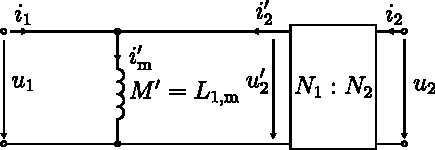
\includegraphics{ex03/ex_transformer_T_ECD_core_losses_no_load.pdf}
    \caption{Equivalent circuit diagram without leakage flux and neglected winding and iron losses.}
    \label{fig:ex_transformer_T_ECD_core_losses_no_load}
  \end{solutionfigure}


  Therefore, the relationship between the voltage and flux linkage is given with:
  \begin{equation}
    u_{\mathrm{1}}(t) = -\frac{\mathrm{d}}{\mathrm{d}t} \psi(t),
  \end{equation}
  which is rearranged into the following form:
  \begin{equation}
    \psi = - \int u_{\mathrm{1}}(t) \mathrm{d}t
    = - \int \sqrt{2} U_{\mathrm{1}} \sin(\omega t) \mathrm{d}t.
  \end{equation}

  Due to the steady state, the integral is indefinite. This results in:
  \begin{equation}
    \psi = \frac{\sqrt{2}U_{\mathrm{1}}}{\omega} \cos(\omega t).
  \end{equation}

  This is simplified in the case of the maximum value of the flux linkage to:
  \begin{equation}
    \hat{\psi} = \frac{\sqrt{2}U_{\mathrm{1}}}{\omega}.
  \end{equation}

  The relationship between the flux linkage, the number of winding turns and flux is given with:
  \begin{equation}
    \psi = N_{\mathrm{1}} \phi_{\mathrm{1}}.
  \end{equation}


  Hence, the number of turns is calculated with:
  \begin{equation}
    N_{\mathrm{1}} = \frac{\hat{\psi}}{\phi}
    = \frac{\frac{\sqrt{2}U_{\mathrm{1}}}{\omega}}{\hat{B} S_{\mathrm{Fe}}}
    =\frac{\frac{\sqrt{2} \cdot \SI{230}{V}}{2\pi \cdot \SI{50}{\hertz}}}{\SI{0.8}{T} \cdot \SI{6\cdot 10^{-4}}{m}}
    = 2157.
    \label{eq:eq1}
  \end{equation}


  The turn ratio of the transformer is defined as follows
  \begin{equation}
    \ddot{u} = \frac{U_{\mathrm{1}}}{U_{\mathrm{2}}}
    = \frac{\SI{230}{\volt}}{\SI{48}{\volt}}
    = 4.79,
  \end{equation}
  hence, the winding turns for the secondary winding are calculated by:
  \begin{equation}
    N_{\mathrm{2}} = \frac{N_{\mathrm{1}}}{\ddot{u}}
    = \frac{2157}{4.79}
    = 451.
  \end{equation}

\end{solutionblock}


%%%%%%%%%%%%%%%%%%%%%%%%%%%%%%%%%%%%%%%%%%%%%%%%%%%%%%%%%%%%%
\subtask{Which magnetization current $I_{\mathrm{m}}'$ consumed the transformer in the no-load operating mode? Assume that the iron losses are neglected.}

\begin{solutionblock}
  
  At no-load operation, the current through the secondary winding is assumed to zero ($i_{\mathrm{2}} = \SI{0}{\ampere}$).
  
  Therefore, the electromotive force simplifies to:
  \begin{equation}
    \theta = H_{\mathrm{Fe}} l_{\mathrm{Fe}}
    = N_{\mathrm{1}} i_{\mathrm{1}}.
  \end{equation}

  Due to the no-load operation, the current through the primary winding is equal to the magnetization current. In addition, the maximum flux density $\hat{B}$ leads to the calculation of the peak magnetization current as:
  \begin{equation}
    \hat{i}_{\mathrm{1}} = \hat{i}_{\mathrm{m,1}}'
    = \frac{\hat{H}_{\mathrm{Fe}} l_{\mathrm{Fe}}}{N_{\mathrm{1}}}
    = \frac{\SI{2}{\ampere \per \centi \metre} \cdot \SI{30}{\centi \metre}}{2157}
    = \SI{27.8}{\milli \ampere}.
  \end{equation}


  The magnetic flux density $B$ shows a linear behavior in the area between 0 T and 0.8 T. Therefore, the magnetization current is not distorted due to the magnetization and has a sinusoidal characteristic.
  Hence, the current is calculated as follows:
  \begin{equation}
    I_{\mathrm{m}}' = \frac{\hat{i}_{\mathrm{m,1}}'}{\sqrt{2}}
    = \frac{\SI{27.8}{\milli\ampere}}{\sqrt{2}}
    = \SI{19.7}{\milli \ampere}.
  \end{equation}

  

\end{solutionblock}


%%%%%%%%%%%%%%%%%%%%%%%%%%%%%%%%%%%%%%%%%%%%%%%%%%%%%%%%%%%%%
\subtask{Calculate the factor between the peak magnetization current $\hat{i}_{\mathrm{m,2}}'$, when the applied voltage is risen from $U_{\mathrm{1}}$ = 230 V to $U_{\mathrm{1}}$ = 400 V.}

\begin{solutionblock}
  With the rearranged equation \eqref{eq:eq1}, the maximum flux density is calculated by:
  \begin{equation}
    \hat{B} = \frac{\sqrt{2} U_{\mathrm{1}}}{\omega S_{\mathrm{Fe}} N_{\mathrm{1}}}
    = \frac{\sqrt{2} \cdot \SI{400}{\volt}}{2\pi \cdot \SI{50}{\hertz} \cdot \SI{6 \cdot 10^{-4}}{\metre} \cdot 2157}
    = \SI{1.39}{\tesla}.
  \end{equation}

  The maximum flux density is used to determine the maximum field strength $\hat{H} = \SI{16}{\ampere \per \centi \metre}$. Hence, the peak magnetization current results in:
  \begin{equation}
    \hat{i}_{\mathrm{m,2}}' = \frac{\hat{H}_{\mathrm{Fe}} l_{\mathrm{Fe}}}{N_{\mathrm{1}}}
    = \frac{\SI{16}{\ampere \per \centi \metre} \cdot \SI{30}{\centi \metre}}{2157}
    = \SI{222.5}{\milli\ampere}.
  \end{equation}

  Hence, the factor is calculated as:
  \begin{equation}
    \frac{\hat{i}_{\mathrm{m,2}}}{\hat{i}_{\mathrm{m,1}}} = \frac{\SI{222.5}{\milli\ampere}}{\SI{27.8}{\milli\ampere}}
    = 8.
  \end{equation}
\end{solutionblock}



%%%%%%%%%%%%%%%%%%%%%%%%%%%%%%%%%%%%%%%%%%%%%%%%%%%%%%%%%%%%%
%% Task 4 %%
%%%%%%%%%%%%%%%%%%%%%%%%%%%%%%%%%%%%%%%%%%%%%%%%%%%%%%%%%%%%%

\task{Parameter identification via no-load test}
Given is a 50 Hz, 6 MVA single-phase transformer with $U_{\mathrm{1}}$ = 5 kV and $U_{\mathrm{2}}$ = 100 kV.
The effective area of the core is $S_{\mathrm{Fe}}$ = 0.187 $\mathrm{m}^2$ and a maximum flux density of $\hat{B}$ = 1.5 T. During the no-load operation, the primary voltage is $U_{\mathrm{1,o}}$ = 5 kV with a no-load electrical power $P_{\mathrm{o}}$ = 8.8 kW and the no-load current $I_{\mathrm{o}}$ = 2.6 A.



%%%%%%%%%%%%%%%%%%%%%%%%%%%%%%%%%%%%%%%%%%%%%%%%%%%%%%%%%%%%%
\subtask{Calculate the nominal currents and the transformer ratio.}

\begin{solutionblock}
  The transformer ratio is given as:
  \begin{equation}
    \ddot{u} = \frac{U_{\mathrm{1}}}{U_{\mathrm{2}}}
    = \frac{\SI{5}{\kilo \volt}}{\SI{100}{\kilo \volt}}
    = 0.05.
  \end{equation}

  With the apparent power $S$ of the transformer, the primary and secondary currents are calculated by:
  \begin{align}
    \begin{split}
      I_{\mathrm{1}} &= \frac{S}{U_{\mathrm{1}}}
      = \frac{\SI{6}{\mega \volt \ampere}}{\SI{5}{\kilo \volt}}
      = \SI{1200}{\ampere}, \\
      I_{\mathrm{2}} &= \frac{S}{U_{\mathrm{2}}}
      = \frac{\SI{6}{\mega \volt \ampere}}{\SI{100}{\kilo \volt}}
      = \SI{60}{\ampere}. \\
    \end{split}
  \end{align}

\end{solutionblock}



%%%%%%%%%%%%%%%%%%%%%%%%%%%%%%%%%%%%%%%%%%%%%%%%%%%%%%%%%%%%%
\subtask{Calculate the number of winding turns $N_{\mathrm{1}}$ for the primary and $N_{\mathrm{2}}$ for the secondary side.}

\begin{solutionblock}
  
  The number of winding turns for the primary side is calculated with:
  \begin{equation}
    N_{\mathrm{1}} = \frac{\hat{\psi}}{\phi}
    = \frac{\frac{\sqrt{2}U_{\mathrm{1}}}{\omega}}{\hat{B} S_{\mathrm{Fe}}}
    = \frac{\frac{\sqrt{2} \cdot \SI{5}{\kilo\volt}}{2\pi \cdot \SI{50}{\hertz}}}{\SI{1.5}{\tesla} \cdot \SI{0.187}{\metre^2}}
    = 81.
    \end{equation}

    The number of winding turns for the secondary side is calculated with the transformer ratio as follows:
    \begin{equation}
      N_{\mathrm{2}} = \frac{N_{\mathrm{1}}}{\ddot{u}}
      = \frac{81}{0.05}
      = 1620.
    \end{equation}
\end{solutionblock}

%%%%%%%%%%%%%%%%%%%%%%%%%%%%%%%%%%%%%%%%%%%%%%%%%%%%%%%%%%%%%
\subtask{Determine the iron losses and the apparent power $S_{\mathrm{o}}$ for no-load operation. Give the values for the magnetization current $I_{\mathrm{m}}'$, the iron loss current $I_{\mathrm{c}}$ and the mutual inductance $M'$. Assume for the calculation that $R_{\mathrm{1}} << R_{\mathrm{c}}$ and $L_{\mathrm{1,\sigma}} << M'$. In addition, draw the equivalent circuit diagram with the given assumptions.}


\begin{solutionblock}

  The equivalent circuit diagram for the no-load operation with the iron loss resistance $R_{\mathrm{c}}$ is shown in \autoref{fig:ex_transformer_open_circuit_test}.
  \begin{solutionfigure}[ht!]
    \centering
    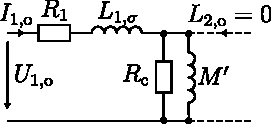
\includegraphics{ex03/ex_Transformer_open_circuit_test.pdf}
    \captionsetup{labelfont={color=blue},textfont={color=blue}}
    \caption{Equivalent circuit diagram for the no-load test with the iron loss resistor $R_{\mathrm{c}}$.}
    \label{fig:ex_transformer_open_circuit_test}
  \end{solutionfigure}
  
  
  The no-load apparent power is calculated by
  \begin{equation}
    S_{\mathrm{o}} = U_{\mathrm{o}} I_{\mathrm{o}}
    = \SI{5}{\kilo\volt} \cdot \SI{2.6}{\ampere}
    = \SI{13}{\kilo\volt\ampere},
  \end{equation}
  with the no-load voltage $U_{\mathrm{o}}$ and the no-load current $I_{\mathrm{o}}$.

  The equivalent iron loss resistance is determine as follows
  \begin{equation}
    R_{\mathrm{c}} = \frac{U_{\mathrm{1,o}}^2}{P_{\mathrm{1,o}}}
    = \frac{\left(\SI{5}{\kilo\volt} \right)^2}{\SI{8.8}{\kilo\watt}}
    = \SI{2841}{\Omega},
  \end{equation}
  and, therefore, the corresponding current is calculated with:
  \begin{equation}
    I_{\mathrm{c}} = \sqrt{\frac{P_{\mathrm{1,o}}}{R_{\mathrm{c}}}}
    = \sqrt{\frac{\SI{8.8}{\kilo\watt}}{\SI{2841}{\Omega}}}
    = \SI{1.76}{\ampere}.
  \end{equation}

  The power factor is determined as
  \begin{equation}
    \cos \varphi_{\mathrm{o}} = \frac{P}{S}
    = \frac{\SI{8.8}{\kilo\watt}}{\SI{13}{\kilo\volt\ampere}}
    = 0.68,
  \end{equation}
  and the corresponding angle is $\varphi_{\mathrm{o}} = \SI{47.16}{\degree}$.

  The following equation is used to calculate the mutual inductance
  \begin{equation}
    \omega_{\mathrm{el}} M' \approx \frac{U_{\mathrm{1,o}}}{I_{\mathrm{1,o}} \sin(\varphi_{\mathrm{o}})},
  \end{equation}
  which is rearranged to:
  \begin{equation}
    M' = \frac{U_{\mathrm{1,o}}}{I_{\mathrm{1,o}} \sin(\varphi_{\mathrm{o}}) \omega_{\mathrm{el}}}
    = \frac{\SI{5}{\kilo\volt}}{\SI{2.6}{\ampere}\cdot \sin(\SI{47.16}{\degree})\cdot 2\pi \cdot \SI{50}{\hertz}}
    = \SI{8.35}{\henry}.
  \end{equation}

  With the geometric addition the magnetization currents is calculated with:
  \begin{equation}
    I_{\mathrm{m}}' = \sqrt{I_{\mathrm{1,o}}^2 - I_{\mathrm{c}}^2}
    = \sqrt{\left(\SI{2.6}{\ampere} \right)^2 - \left(\SI{1.76}{\ampere}\right)^2}
    = \SI{1.91}{\ampere}.
  \end{equation}

\end{solutionblock}







%%%%%%%%%%%%%%%%%%%%%%%%%%%%%%%%%%%%%%%%%%%%%%%%%%%%%%%%%%%%%
%% Task 5 %%
%%%%%%%%%%%%%%%%%%%%%%%%%%%%%%%%%%%%%%%%%%%%%%%%%%%%%%%%%%%%%

\task{Inrush current}
Given is a single-phase transformer in no-load operation (i.e., open circuit secondary side) which initial primary current is zero. A the time point $t$ = 0, the voltage $u_{\mathrm{n}}(t) = \hat{u}_{\mathrm{n}} \sin (\omega t + \alpha)$ is applied.
Remanence and iron losses are neglected.
The self-inductance $L_{\mathrm{1}}$, resistance $R_{\mathrm{1}}$ and the number of winding turns $N_{\mathrm{1}}$ are given.

%%%%%%%%%%%%%%%%%%%%%%%%%%%%%%%%%%%%%%%%%%%%%%%%%%%%%%%%%%%%%
\subtask{Calculate the inrush current trajectory $i_{\mathrm{1}}(t)$ and the trajectory of the flux $\phi (t)$.}

\begin{solutionblock}
  
  The dynamic equation of the transformer current is given as follows:
  \begin{equation}
    \frac{\mathrm{d}}{\mathrm{d}t}\bm{i}(t) = \begin{bmatrix} -\frac{R_1}{\sigma L_1} & \frac{R_2 M}{\sigma L_1 L_2} \\ \frac{R_1 M}{\sigma L_1 L_2} & -\frac{R_2}{\sigma L_2} \end{bmatrix} \bm{i}(t) + \begin{bmatrix} \frac{1}{\sigma L_1} & -\frac{M}{\sigma L_1 L_2} \\ -\frac{M}{\sigma L_1 L_2} & \frac{1}{\sigma L_2} \end{bmatrix} \bm{u}(t).
  \end{equation}

  Due to the no-load operation ($i_{\mathrm{2}} = \SI{0}{\ampere}$) and the neglected leakage flux, the equation simplifies to:
  \begin{equation}
    \frac{\mathrm{d}}{\mathrm{d}t} i_{\mathrm{1}}(t) = -\frac{R_{\mathrm{1}}}{L_{\mathrm{1}}}i_{\mathrm{1}}(t) -\frac{1}{L_{\mathrm{1}}} u_{\mathrm{1}}(t).
  \end{equation}

  The equation from above is rearranged to solve the ordinary differential equation. Therefore, the homogeneous part is on the left side and the perturbation part on the right side as given below
  \begin{equation}
    \frac{\mathrm{d}}{\mathrm{d}t} i_{\mathrm{1}}(t) + \frac{1}{\tau} i_{\mathrm{1}}(t) = \frac{1}{L_{\mathrm{1}}} u_{\mathrm{1}}(t),
    \label{eq:ode}
  \end{equation}
  with $\tau = \frac{L_{\mathrm{1}}}{R_{\mathrm{1}}}$.
  
  First, the homogeneous part is separated, which results in:
  \begin{equation}
    \frac{\mathrm{d}}{\mathrm{d}t} i_{\mathrm{1}}(t) + \frac{1}{\tau} i_{\mathrm{1}}(t) = 0.
  \end{equation}

  This homogeneous part is solved with the exponential approach, which is given with
  \begin{equation}
    i_{\mathrm{1}}(t) = C e^{-\frac{t}{\tau}},
    \label{eq:ode_approach_hom}
  \end{equation}
  and the first derivative
  \begin{equation}
    \frac{\mathrm{d}}{\mathrm{d}t}i_{\mathrm{1}}(t) = -\frac{C}{\tau} e^{-\frac{t}{\tau}},
    \label{eq:ode_approach_hom_derivative}
  \end{equation}
  with an integration constant $C$.

  Using \eqref{eq:ode_approach_hom} and \eqref{eq:ode_approach_hom_derivative} results in
  \begin{equation}
    \frac{R_{\mathrm{1}}}{L_{\mathrm{1}}} C e^{-\frac{t}{\tau}} - \frac{C}{\tau} e^{-\frac{t}{\tau}} = 0,
  \end{equation}
  which is rearranged as follows:
  \begin{equation}
    C e^{-\frac{t}{\tau}} \left(\frac{R_{\mathrm{1}}}{L_{\mathrm{1}}}-\frac{t}{\tau} \right)=0.
  \end{equation}


  Therefore, the homogeneous solution is given as:
  \begin{equation}
    i_{\mathrm{1,h}}(t) = C e^{-\frac{t}{\tau}}.
  \end{equation}
  

  In the second step, the perturbation solution is determined. Therefore, the comparison of coefficients ansatz is used.
  The voltage is given in the task with
  \begin{equation}
    u_{\mathrm{n}} = \hat{u}_{\mathrm{n}} \sin(\omega t + \alpha),
  \end{equation}
  which leads to:
  \begin{equation}
    \sin(\omega t + \alpha) = \cos(\omega t) \sin(\alpha) + \sin(\omega t) \cos(\alpha).
    \label{eq:ode_perturbation}
  \end{equation}

  The expression in \eqref{eq:ode_perturbation} is separated in two parts which are later combined again (superposition principle of linear systems). The approach for the first case is given by:
  \begin{equation}
    \frac{\mathrm{d}}{\mathrm{d}t}i(t) + \frac{1}{\tau}i(t) = k \sin(\alpha) \cos(\omega t),
  \end{equation}
  with a new parameter $k = \frac{\hat{u}}{L_{\mathrm{1}}}$, derived from \eqref{eq:ode}.

  The general approach is given with
  \begin{equation}
    i_{\mathrm{1,s}}(t) = a \cos(\omega t) + b \sin(\omega t),
    \label{eq:ode_approach_per}
  \end{equation}
  with the two parameter $a$ and $b$. The first derivative is determined as:
  \begin{equation}
    \frac{\mathrm{d}}{\mathrm{d}t} i_{\mathrm{1,s}}(t) = - a \omega \sin(\omega t) + b \omega \cos(\omega t).
    \label{eq:ode_approach_per_derivative}
  \end{equation}

  With \eqref{eq:ode_approach_per} and \eqref{eq:ode_approach_per_derivative} in \eqref{eq:ode} the equation is determined:
  \begin{equation}
    - a \omega \sin(\omega t) + b \omega \cos(\omega t) + \frac{1}{\tau} \left[a \cos(\omega t) + b \sin(\omega t)  \right]
    = k \sin(\alpha) \cos(\omega t).
  \end{equation}

  The following equation is obtained by reshaping
  \begin{equation}
    \sin(\omega t) \left[-a \omega + \frac{1}{\tau} b \right] + \cos(\omega t) \left[b\omega + \frac{1}{\tau} a - k \sin(\omega t) \right] = 0,
  \end{equation}
  and by dividing through $\cos(\omega t)$ results in:
  \begin{equation}
    \tan(\omega t) \left[-a \omega + \frac{1}{\tau} b \right] + \left[b \omega + \frac{1}{\tau}a - k \sin(\omega t) \right] = 0.
  \end{equation}

  To fulfill the equation, the expressions between the large brackets must be zero. 
  The first expression is given with:
  \begin{align}
    \begin{split}
      -a\omega + &\frac{1}{\tau}b = 0, \\
      b &= a \omega \tau.
      \label{eq:ode_b}
    \end{split}
  \end{align}

  The second expression is defined with:
  \begin{equation}
    b \omega + \frac{1}{\tau} a - k \sin(\alpha) = 0.
  \end{equation}

  With $b$ from \eqref{eq:ode_b} results in
  \begin{align}
    \begin{split}
      a \omega^2 \tau + \frac{1}{\tau} a - k \sin(\alpha) = 0, \\
      a \left[\omega^2 \tau + \frac{1}{\tau} \right] = k \sin(\alpha),
    \end{split}
  \end{align}

  which is reshaped to:
  \begin{equation}
    a = \frac{k \sin(\alpha)}{\omega^2 \tau + \frac{1}{\tau}}.
  \end{equation}

  Therefore, with the two calculated coefficients, the solution for the first approach is: 
  \begin{equation}
    i_{\mathrm{1,s}}(t) = \frac{k \sin(\alpha)}{\omega^2 \tau + \frac{1}{\tau}} \left[\cos(\omega t) + \omega \tau \sin(\omega t) \right].
  \end{equation}


  The second case is given with $\frac{\mathrm{d}}{\mathrm{d}t}i(t) + \frac{1}{\tau}i(t) = k \cos(\alpha) \sin(\omega t)$.To do this, the steps already carried out in the first approach are repeated.
  The starting point is given as
  \begin{equation}
    i_{\mathrm{2,s}}(t) = a \cos(\omega t) + b \sin(\omega t),
  \end{equation}
  and, therefore, the first derivative:
  \begin{equation}
    \frac{\mathrm{d}}{\mathrm{d}t} i_{\mathrm{2,s}}(t) = - a \omega \sin(\omega t) + b \omega \cos(\omega t).
  \end{equation}

  The comparison of coefficients and reshaping leads to:
  \begin{align}
    \begin{split}
    -a \omega \sin(\omega t) + b \omega \cos(\omega t) = \frac{1}{\tau} \left[a \cos(\omega t) + b\sin(\omega t) \right] &= k \sin(\omega t), \\
    \sin(\omega t) \left[-a \omega + \frac{1}{\tau}b - k\cos(\alpha)\right] + \cos(\omega t) \left[b \omega + \frac{1}{\tau}a \right] &= 0.
    \end{split}
  \end{align}

  To fulfill the equation, the expressions between the large brackets must be zero. 
  The first expression is given with:
  \begin{align}
    \begin{split}
      b \omega + &\frac{1}{\tau}a =0, \\
      a &= \omega b \tau.
      \label{eq:ode_parameter_a}
    \end{split}
  \end{align}

  The second expression is defined with:
  \begin{align}
    \begin{split}
      -a \omega + &\frac{1}{\tau}b - k\cos(\alpha) = 0, \\
      \omega^2 b \tau + &\frac{1}{\tau}b - k \cos(\alpha) = 0, \\
      b &= \frac{k\cos(\alpha)}{\omega^2\tau+\frac{1}{\tau}}.
    \end{split}
  \end{align}

  This result is used to solve parameter $a$ from \eqref{eq:ode_parameter_a} as follows:
  \begin{equation}
    a = -\omega b \tau = -\frac{\omega \tau k \cos(\alpha)}{\omega^2\tau + \frac{1}{\tau}}.
  \end{equation}

  Therefore, the solution for the second case of the perturbation part is defined as
  \begin{equation}
    i_{\mathrm{s,2}}(t) = \frac{k\cos(\alpha)}{\omega^2 \tau + \frac{1}{\tau}} \left[-\omega \tau \cos(\omega t) + \sin(\omega t) \right],
    \end{equation}

 and, this leads to the solution of the perturbation part by:
  \begin{equation}
    i_{\mathrm{1,s}}(t) = \frac{k}{\omega^2 \tau + \frac{1}{\tau}}
    \left[
      \sin(\alpha)\left[\cos(\omega t) + \omega \tau \sin(\omega t) \right]
      + \cos(\alpha) \left[-\omega \tau \cos(\omega t) + \sin(\omega t) \right]
    \right].
  \end{equation}

  The total solution is given with:
  \begin{equation}
    i_{\mathrm{1}}(t) = i_{\mathrm{1,h}}(t) + i_{\mathrm{1,s}}(t).
  \end{equation}


  Next, the integration constant $C$ from the homogeneous solution is determined. To perform this, the initial conditions are used, which are defined in the task description. Therefore, the current is defined as:
  \begin{equation}
    i_{\mathrm{1}}(0) = 0.
    \label{eq:ode_initialCondition}
  \end{equation}
  
  The second initial condition is the results of applying \eqref{eq:ode_initialCondition} to the differential equation, that is:
  \begin{equation}
    \frac{\mathrm{d}}{\mathrm{d}t}i_{\mathrm{1}}(0) = \frac{1}{L_{\mathrm{1}}}u(0) = \frac{1}{L_{\mathrm{1}}} \hat{u}\sin(\alpha).
  \end{equation}

  Apply the initial conditions to the total solution results in
  \begin{equation}
    i(0) = C + \frac{k}{\omega^2 \tau + \frac{1}{\tau}}
    \left[\sin(\alpha) - \omega \tau \cos(\alpha) \right] = 0,
  \end{equation}
  which is rearranged to:
  \begin{equation}
    C = \frac{k}{\omega^2\tau + \frac{1}{\tau}} \left[-\sin(\alpha) + \omega \tau \cos(\alpha) \right].
  \end{equation}

  Therefore, the total solution is given with:
  \begin{align}
    \begin{split}
      i_{\mathrm{1}}(t) &=\frac{k}{\omega^2\tau + \frac{1}{\tau}} \left[-\sin(\alpha) + \omega \tau \cos(\alpha) \right] e^{-\frac{t}{\tau}} \\
      &+\frac{k}{\omega^2 \tau + \frac{1}{\tau}}
      \left[
        \sin(\alpha)\left[\cos(\omega t) + \omega \tau \sin(\omega t) \right]
        + \cos(\alpha) \left[-\omega \tau \cos(\omega t) + \sin(\omega t) \right]
      \right].
      \label{eq:ode_solution}
  \end{split}
  \end{align}

  The trajectory of the flux is defined as
  \begin{equation}
    \phi(t) = L_{\mathrm{1}} i(t),
  \end{equation}
  and, therefore, directly given with the current trajectory.
\end{solutionblock}



%%%%%%%%%%%%%%%%%%%%%%%%%%%%%%%%%%%%%%%%%%%%%%%%%%%%%%%%%%%%%
\subtask{Assume that $R_{\mathrm{1}} << \omega L_{\mathrm{1}}$.
Discuss the result for $i_{\mathrm{1}}(t)$, when the voltage is applied at zero crossing with an angle $\alpha$ = 0 and for an angle of $\alpha = \frac{\pi}{2}$.}

\begin{solutionblock}

  First, the trajectory for $\alpha$ = 0 is determined. Therefore, \eqref{eq:ode_solution} results in:
  \begin{equation}
    i_{\mathrm{1}}(t) = \frac{k}{\omega^2\tau+\frac{1}{\tau}} \left[\omega \tau e^{-\frac{t}{\tau}} - \omega \tau \cos(\omega t) + \sin(\omega t) \right].
  \end{equation}

  With the assumptions given in the task, $R_{\mathrm{1}} << L_{\mathrm{1}} \omega$
  results into $\omega \tau >> 1$.

  Hence, the equation simplifies to
  \begin{align}
    \begin{split}
      i_{\mathrm{1}}(t) &= \frac{k}{\omega^2\tau + \frac{1}{\tau}} \omega t \left[e^{-\frac{t}{\tau}} - \cos(\omega t) \right], \\
      &= \frac{\hat{u}}{L_{\mathrm{1}}} \frac{1}{\omega} \left[e^{-\frac{t}{\tau}} - \cos(\omega t) \right],
    \end{split}
  \end{align}
  which is used to calculate the current trajectory. 
  As it can be seen, the equation contains an exponential part. To determine the steady-state current trajectory, the equation is reshaped into:
  \begin{align}
    \begin{split}
    i_{\mathrm{1}}(t) = \frac{\hat{u}}{L_{\mathrm{1}}\omega}e^{-\frac{t}{\tau}}-\frac{\hat{u}}{L_{\mathrm{1}}\omega}\cos(\omega t), \\
    = \frac{\hat{u}}{L_{\mathrm{1}}\omega}e^{-\frac{t}{\tau}} + \frac{\hat{u}}{L_{\mathrm{1}}} \int \sin(\omega t) \mathrm{d}t.
    \end{split}
  \end{align}

  With the input voltage $u(t) = \hat{u}\sin(\omega t + \alpha)$, the equation simplifies to:
  \begin{equation}
    i_{\mathrm{1}}(t) = \frac{\hat{U}}{L_{\mathrm{1}}\omega}e^{-\frac{t}{\tau}} + \frac{1}{L_{\mathrm{1}}} \int u(t) \mathrm{d}t.
  \end{equation}

  Assumed, that in the steady state $\tau \rightarrow \infty$, only the second part of the equation remains. Therefore, the current trajectory is given with:
  \begin{equation}
    i_{\mathrm{1}}(t) = \frac{1}{L_{\mathrm{1}}} \int u(t) \mathrm{d}t.
  \end{equation}

  Next, the trajectory for $\alpha = \frac{\pi}{2}$ is determined. Therefore, the equation \eqref{eq:ode_solution} is solved as follows:
  \begin{align}
    \begin{split}
      i_{\mathrm{1}}(t) &= \frac{k}{\omega^2\tau + \frac{1}{\tau}}
      \left[\cos(\omega t) + \omega \tau \sin(\omega t) \right], \\
      &= \frac{k}{\omega^2\tau + \frac{1}{\tau}} \left[\omega \tau \sin(\omega t) \right], \\
      &= \frac{1}{L_{\mathrm{1}}} \hat{U} \frac{1}{\omega} \sin(\omega t), \\
      &= \frac{\hat{U}}{L_{\mathrm{1}}\omega} \sin(\omega t).
    \end{split}
  \end{align}


  In \autoref{fig:current_transformer} the two calculated current trajectories are visualized. They result from the applied voltage with the additional angle $\alpha$.
  In this example is the peak current value during the transient process approximately double than in the steady state, which can trigger the overcurrent protection. Therefore, the magnetization current should be kept low and the overcurrent protection must be able to handle the inrush current.
  \begin{solutionfigure}[ht!]
    \centering
    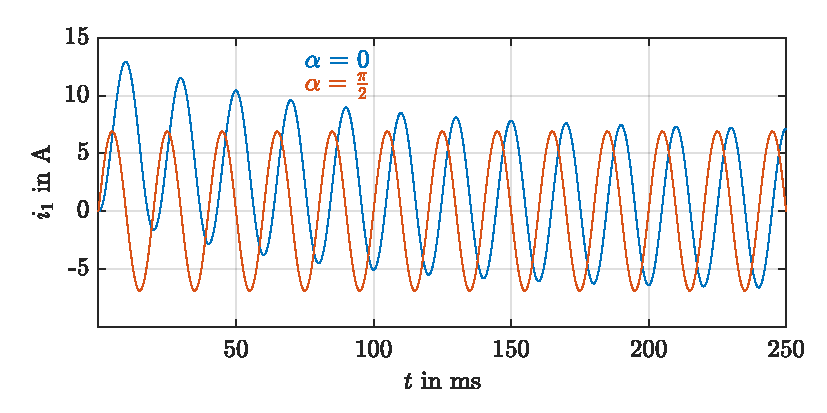
\includegraphics{ex03/current_transformer.pdf}
    \caption{Current of the transformer, when the voltage is applied at two different angles for $\alpha$.}
    \label{fig:current_transformer}
  \end{solutionfigure}
  

\end{solutionblock}
    %%%%%%%%%%%%%%%%%%%%%%%%%%%%%%%%%%%%%%%%%%%%%%%%%%%%%%%%%%%%%
%% Begin exercise %%
%%%%%%%%%%%%%%%%%%%%%%%%%%%%%%%%%%%%%%%%%%%%%%%%%%%%%%%%%%%%%
\ex{Fourier analysis of rotating fields}


\normalsize{\textbf{Acknowledgement}: The following exercise is adapted from ``Geregelte Drehstromantriebe / Controlled AC Drives'' by J. Böcker, Paderborn University, 2021 and 
``Elektrische Maschinen und Antriebe Übungsbuch: Aufgaben mit Lösungsweg'' by A. Binder, Springer, 2017
}\\



%%%%%%%%%%%%%%%%%%%%%%%%%%%%%%%%%%%%%%%%%%%%%%%%%%%%%%%%%%%%%
%% Task 1 %%
%%%%%%%%%%%%%%%%%%%%%%%%%%%%%%%%%%%%%%%%%%%%%%%%%%%%%%%%%%%%%

\task{Fourier analysis of a field distribution of a three-phase winding}
The winding of a three-phase and four-pole machine is described with the following parameters. The number of notches is given with $q$ = 2 and the winding chording is $y/\rho_{\mathrm{p}}$ = 5/6. The number of windings per coil is given with $N_{\mathrm{c}}$ = 5 with $a$ = 1. The air gap is given with $\delta$ = 1 mm and the inner stator diameter is $d_{\mathrm{s}}$ = 80 mm. The phase current root mean square value is given with $I_{\mathrm{s}}$ = 30  A.

%%%%%%%%%%%%%%%%%%%%%%%%%%%%%%%%%%%%%%%%%%%%%%%%%%%%%%%%%%%%%
\subtask{Calculate the number of slots per pole pair. In addition, determine the pole pitch $\rho_{\mathrm{p}}$ as an angular information and calculate the pole pitch $\tau_{\mathrm{p}}$ as a distance in m. Furthermore, determine the number of conductors per phase.}

\begin{solutionblock}
    The number of slots is calculated with
    \begin{equation}
        Q = q 2 p m
        = 2\cdot 2\cdot 2\cdot 3
        = 24,
    \end{equation}
    where $p$ is the number of pole pairs and $m$ is the number of phases. Therefore, the number of slots per pole pair is given with:
    \begin{equation}
        \frac{Q}{p} = \frac{24}{2} = 12.
    \end{equation}

    The pole pitch as an angular information is calculated with
    \begin{equation}
        \rho_{\mathrm{p}} = \frac{\pi}{p}
        = \frac{\pi}{2},
    \end{equation}
    and in comparison, the pole pitch as a distance information is determined as:
    \begin{equation}
        \tau_{\mathrm{p}} = \frac{d_{\mathrm{s}}\pi}{2p}
        = \frac{\SI{80}{\milli \metre \cdot \pi}}{2 \cdot 2}
        = \SI{62.8}{\milli\metre}.
    \end{equation}

    The conductors per phase are calculated by:
    \begin{equation}
        N_{\mathrm{a}} = \frac{2pqN_{\mathrm{c}}}{a}
        = \frac{2\cdot 2\cdot 2\cdot 5}{1}
        = 40.
    \end{equation}
\end{solutionblock}


%%%%%%%%%%%%%%%%%%%%%%%%%%%%%%%%%%%%%%%%%%%%%%%%%%%%%%%%%%%%%
\subtask{Calculate the amplitude of the flux density fundamental in the air gap assuming an ideal homogenous and block-shaped flux distribution along the stator circumference.}

\begin{solutionblock}
    The maximum flux density is given with:
    \begin{equation}
        \hat{B} = \frac{\mu_{\mathrm{0}}N \hat{i}}{2 \delta}
        = \frac{\SI{4\pi\cdot10^{-7}}{\volt\second\per\ampere\metre}\cdot 40 \cdot \SI{\left(30\cdot \sqrt{2} \right)}{\ampere}}{2\cdot \SI{0.001}{\metre}}
        = \SI{1.07}{\volt\second}.
    \end{equation}

    The general form to calculate the flux density for phase a of a harmonic order is defined by
    \begin{equation}
        \hat{B}_{\mathrm{a}}^{(k)}(t) = \frac{4}{\pi} \hat{B} \cos(\omega t) \frac{1}{k} \xi_{\mathrm{d,}k} \xi_{\mathrm{p,}k},
        \label{eq:harmonicOrderFluxDensity}
    \end{equation}
    with $\xi_{\mathrm{d,}k}$ is the distribution and $\xi_{\mathrm{p,}k}$ is the pitch factor. Hence, for the fundamental wave is $k$ = 1, which leads to
    \begin{equation}
        \xi_{\mathrm{d,}1} = \frac{\sin\left( \frac{1\cdot \pi}{2m}\right)}{q\sin\left(\frac{1\cdot\pi}{2mq}\right)}
        = \frac{\sin\left(\frac{1\cdot\pi}{2\cdot3}\right)}{2\cdot \sin\left(\frac{1\cdot\pi}{2\cdot3\cdot2}\right)}
        = 0.966,
        \label{eq:distributionFactor}
    \end{equation}
    and,
    \begin{equation}
        \xi_{\mathrm{p,}1} = \sin\left(1\cdot \frac{\pi}{2} \frac{y}{\rho_{\mathrm{p}}} \right)
        = \sin\left(1 \cdot \frac{\pi}{2} \cdot \frac{5}{6} \right)
        = 0.966.
        \label{eq:pitchFactor}
    \end{equation}

    Finally, \eqref{eq:harmonicOrderFluxDensity} is multiplied by a factor of $\frac{3}{2}$ to calculate the amplitude of the fundamental wave of the three phases acting on the air gap flux. This leads to:
    \begin{equation}
        \hat{B}^{(1)} = \frac{3}{2}\cdot\frac{4}{\pi} \cdot \SI{1.07}{\volt\second} \cdot \frac{1}{1} \cdot 0.966 \cdot 0.966
        = \SI{1.27}{\volt\second}.
        \label{eq:Fourier_threePhases}
    \end{equation}

\end{solutionblock}


%%%%%%%%%%%%%%%%%%%%%%%%%%%%%%%%%%%%%%%%%%%%%%%%%%%%%%%%%%%%%
\subtask{Determine the amplitudes of the resulting flux density for the fundamental wave and the following six harmonic orders. Give the results as relative fractions to the amplitude of the fundamental wave. In addition, calculate the distribution, pitch and winding factor for the given harmonics and the fundamental wave.}

\begin{solutionblock}
    The flux density for the harmonic orders is calculated with \eqref{eq:Fourier_threePhases}. The pitch factors are determined with \eqref{eq:pitchFactor} and the distribution factors with \eqref{eq:distributionFactor}. The winding factor is given with:
    \begin{equation}
        \xi_{\mathrm{w,}k} = \xi_{\mathrm{d,}k} \xi_{\mathrm{p,}k}.
    \end{equation}

    For the calculation up to the $19\textsuperscript{th}$ harmonic, a short Python script is written.
    The results are visualized in \autoref{tab:windingFactors}.
    \begin{solutiontable}[ht]
        \caption{Distribution, pitch, and winding factors as well as relative harmonic flux density  amplitudes.}
        \centering
        \begin{tabular}{rcrrr}\toprule
        $k$ & $\frac{\hat{B}^{(k)}}{\hat{B}^{(1)}}$ in \%   & $\xi_{\mathrm{p,}k}$  & $\xi_{\mathrm{d,}k}$ & $\xi_{\mathrm{w,}k}$\\
        \midrule
        1   & 100   & 0.966 & 0.966 & 0.966 \\
        5   & 1.4   & 0.259 & 0.259 & 0.067 \\
        7   & 1.0   & 0.259 & 0.259 & 0.067 \\
        11  & 9.1   & 0.966 & 0.966 & 0.933 \\
        13  & 7.7   & 0.966 & 0.966 & 0.933 \\
        17  & 0.4   & 0.259 & 0.259 & 0.067 \\
        19  & 0.38  & 0.259 & 0.259 & 0.067 \\
        \bottomrule
        \end{tabular}
        \label{tab:windingFactors}
    \end{solutiontable}

\end{solutionblock}

%%%%%%%%%%%%%%%%%%%%%%%%%%%%%%%%%%%%%%%%%%%%%%%%%%%%%%%%%%%%%
\subtask{Sketch the flux density of the fundamental wave in the air gap of phase a as a function of the electrical stator circumference $\vartheta_\mathrm{el}$. Assume $i_a(t) = I_s \cdot \sqrt{2}$, i.e., the phase a is at its current peak. In addition, draw the flux density of the $11\textsuperscript{th}$ harmonic.}

\begin{solutionblock}
    The calculation is performed with \eqref{eq:harmonicOrderFluxDensity} in a separate Python script. The resulting trajectories are shown in \autoref{fig:fundamentalAnd11thHarm}.
    \begin{solutionfigure}[ht]
        \centering
        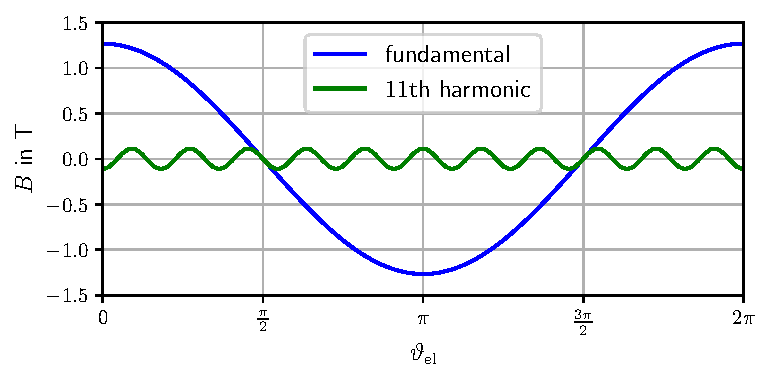
\includegraphics{ex04/FundamentalAnd11thHarmonic.pdf}
        \caption{Visualization of the flux density of the fundamental wave and the $11\textsuperscript{th}$ harmonic of phase~a.}
        \label{fig:fundamentalAnd11thHarm}
    \end{solutionfigure}    

\end{solutionblock}




%%%%%%%%%%%%%%%%%%%%%%%%%%%%%%%%%%%%%%%%%%%%%%%%%%%%%%%%%%%%%
%% Task 2 %%
%%%%%%%%%%%%%%%%%%%%%%%%%%%%%%%%%%%%%%%%%%%%%%%%%%%%%%%%%%%%%

\task{Distributed windings}
Consider a 4-pole three-phase motor with 15 stator slots. A simplified sketch of this motor with the winding scheme of phase a is shown in \autoref{fig:MMF_distributed}.

\begin{figure}[htb]
    \centering
    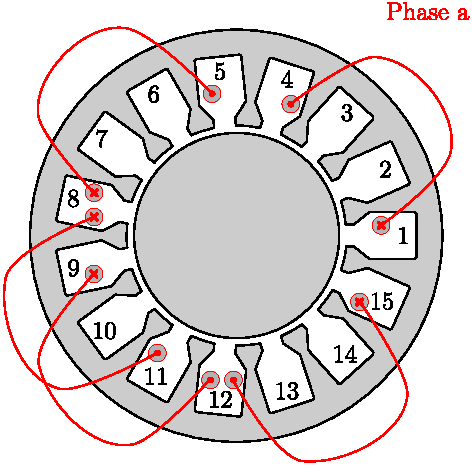
\includegraphics{ex04/MMF_distributed.pdf}
    \caption{Simplified sketch of a distributed winding scheme. Only phase a is shown.}
    \label{fig:MMF_distributed}
\end{figure}



%%%%%%%%%%%%%%%%%%%%%%%%%%%%%%%%%%%%%%%%%%%%%%%%%%%%%%%%%%%%%
\subtask{Determine the pole pitch $\rho_{\mathrm{p}}$ and the number of notches. Is it an integral-slot or a fractional-slot winding?}

\begin{solutionblock}
    The number of slots are shown in the figure, which leads to $Q$ = 15. Furthermore, the number of phases is given in the task, that is $m$ = 3.

    Hence, the pole pitch is calculated as:
    \begin{equation}
        \rho_{\mathrm{p}} = \frac{2\pi}{2p}
        = \frac{\pi}{2}.
    \end{equation}
    
    The number of notches is defined with:
    \begin{equation}
        q = \frac{Q}{2pm} = \frac{15}{2\cdot 2 \cdot 3}
        = \frac{15}{12} = \frac{5}{4}.
    \end{equation}
    Since the number of notches per pole and phase is not an integer, it is a fractional slot winding.
    The coil width $y$ is three stator slots, which leads to the angular coil width:
    \begin{equation}
        w = \frac{2\pi}{Q}m
        = \frac{2\pi}{15} \cdot 3
        = \frac{2\pi}{5}.
    \end{equation}

    Therefore, the chording factor is determined with:
    \begin{equation}
        s = \frac{w}{\tau_{\mathrm{p}}}
        = \frac{6\pi \cdot 2}{15 \pi}
        =\frac{12}{15}.
    \end{equation}

\end{solutionblock}

%%%%%%%%%%%%%%%%%%%%%%%%%%%%%%%%%%%%%%%%%%%%%%%%%%%%%%%%%%%%%
\subtask{Complete the winding scheme of the given machine in \autoref{tab:distributed_winding} for the phases b and c. Sketch the resulting winding scheme into \autoref{fig:MMF_distributed}.}

\begin{table}[ht]
    \caption{Winding scheme of the distributed winding from \autoref{fig:MMF_distributed}.}
    \centering
    \begin{tabular}{c|C{1cm}|C{1cm}|C{1cm}|C{1cm}|C{1cm}|C{1cm}}\toprule
        \multirow{2}{*}{Coil nr.} & \multicolumn{2}{c}{Phase a} & \multicolumn{2}{c}{Phase b} & \multicolumn{2}{c}{Phase c} \\
          & In  & Out   & In & Out & In & Out \\
        \midrule
        1  & 1  & 4  & & & & \\
        2  & 8  & 5  & & & & \\
        3  & 8  & 11 & & & & \\
        4  & 9  & 12 & & & & \\
        5  & 15 & 12 & & & & \\
        \bottomrule
    \end{tabular}
    \label{tab:distributed_winding}
\end{table}

\begin{solutionblock}
    In the task only phase a of the winding scheme is given. However, to complete the winding scheme, phase b must have an electrical phase shift of $\SI{120}{\degree}$ and phase c of $\SI{240}{\degree}$ respectively.
    This leads to
    \begin{equation}
        n_{\mathrm{b}} p \frac{\SI{360}{\degree}}{Q} = \SI{120}{\degree} \ \mathrm{mod} \ \SI{360}{\degree},
    \end{equation}
    where $n_{\mathrm{b}}$ is the displacement in slots. This expression is rewritten into
    \begin{equation}
        n_{\mathrm{b}} p \frac{\SI{360}{\degree}}{Q} = \SI{120}{\degree} + k \SI{360}{\degree},
        \label{eq:nb}
    \end{equation}
    and also for phase c:
    \begin{equation}
        n_{\mathrm{c}} p \frac{\SI{360}{\degree}}{Q} = \SI{240}{\degree} + k \SI{360}{\degree}.
        \label{eq:nc}
    \end{equation}
    
    Now, an integral solution must be found for \eqref{eq:nb} and \eqref{eq:nc} to determine the winding scheme.
    This is done with trial and error, the first assumption is $n_{\mathrm{b}} = 10, k = 1$, which results in
    \begin{align}
        \begin{split}
            10\cdot 2\cdot \frac{\SI{360}{\degree}}{15} &= \SI{120}{\degree}+\SI{360}{\degree}, \\
            \SI{480}{\degree} &= \SI{480}{\degree},
        \end{split}
    \end{align}
    therefore, the requirement is fulfilled. For phase c the assumption is given with $n_{\mathrm{c}} = 5, k = 1$ into \eqref{eq:nc}
    \begin{align}
        \begin{split}
            5 \cdot 2 \cdot \frac{\SI{360}{\degree}}{15} &= \SI{240}{\degree} + k \SI{360}{\degree}, \\
            \SI{240}{\degree} &= \SI{240}{\degree},
        \end{split}
    \end{align}
    which fulfills the requirement too.
    With the calculated phase shift and the knowledge of the coil width of three slots from the figure, the winding scheme is completed.
    In \autoref{tab:solution_distributedWinding} the inputs and outputs of each winding are given.
    \begin{solutiontable}[ht]
        \caption{Solution of the distributed winding scheme.}
        \centering
        \begin{tabular}{c|C{1cm}|C{1cm}|C{1cm}|C{1cm}|C{1cm}|C{1cm}}\toprule
            \multirow{2}{*}{Coil nr.} & \multicolumn{2}{c}{Phase a} & \multicolumn{2}{c}{Phase b} & \multicolumn{2}{c}{Phase c} \\
              & In  & Out   & In & Out & In & Out \\
            \midrule
            1  & 1  & 4  & 11 & 14 & 6  & 9 \\
            2  & 8  & 5  & 3  & 15 & 13 & 10 \\
            3  & 8  & 11 & 3  & 6  & 13 & 1 \\
            4  & 9  & 12 & 4  & 7  & 14 & 2 \\
            5  & 15 & 12 & 10 & 7  & 5  & 2 \\
            \bottomrule
        \end{tabular}
        \label{tab:solution_distributedWinding}
    \end{solutiontable}

    The sketch of the distributed winding scheme is visualized in \autoref{fig:solution_MMF_distributed}.
    \begin{solutionfigure}[ht]
        \centering
        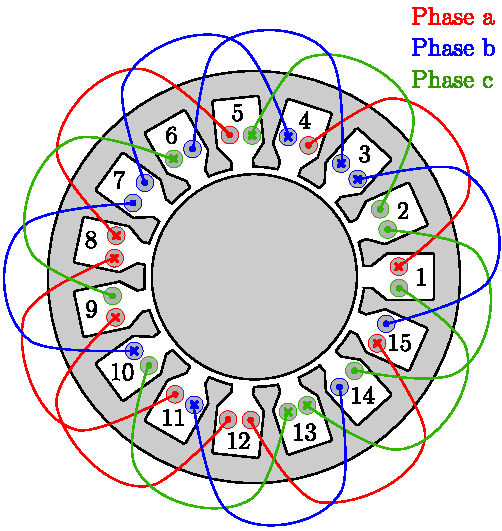
\includegraphics{ex04/solution_MMF_distributed.pdf}
        \caption{Solution of the distributed winding.}
        \label{fig:solution_MMF_distributed}
    \end{solutionfigure}

\end{solutionblock}


%%%%%%%%%%%%%%%%%%%%%%%%%%%%%%%%%%%%%%%%%%%%%%%%%%%%%%%%%%%%%
\subtask{How many layers are there in this winding scheme?}

\begin{solutionblock}
    The winding diagram has 2 winding layers, due to the two conductors per slot.
\end{solutionblock}


%%%%%%%%%%%%%%%%%%%%%%%%%%%%%%%%%%%%%%%%%%%%%%%%%%%%%%%%%%%%%
\subtask{Calculate the complex winding factors $\underline{\xi}_{\mathrm{a,}k}$ for the fundamental as well as for the $5\textsuperscript{th}$ and $7\textsuperscript{th}$ harmonic.}

\begin{solutionblock}
    The complex winding factor is defined by
    \begin{equation}
        \xi_{\mathrm{a,}k} = \frac{1}{\mathrm{j}N_{\mathrm{a}}} \sum_{i=1}^{Q} N_{\mathrm{a,}i}e^{\mathrm{j}k\vartheta_{\mathrm{el,a,}i}},
        \label{eq:complexWindingFactor}
    \end{equation}
    with
    \begin{equation}
        N_{\mathrm{a}} = \sum_{i=1}^{Q} |N_{\mathrm{a,}i} |,
    \end{equation}
    and the electrical angle:
    \begin{equation}
        \vartheta_{\mathrm{el,a,}i} = \vartheta_{\mathrm{a,}i} \cdot p.
    \end{equation}

    The mechanical angles are calculated with
    \begin{equation}
        \vartheta_{\mathrm{a,}i} = \left(i-1 \right) \frac{\SI{360}{\degree}}{Q}
        = \left(i-1 \right) \cdot \frac{\SI{360}{\degree}}{15}
        = \left(i-1 \right) \cdot \SI{24}{\degree},
    \end{equation}
    where $i$ represents the number of the stator slot.
    Therefore, the mechanical angles are given in \autoref{tab:mechanicalAngles_distributedWinding}.
    \begin{solutiontable}[ht]
        \caption{Mechanical angles of the distributed winding from \autoref{fig:MMF_distributed}.}
        \centering
        \begin{tabular}{C{3cm}|C{3cm}}\toprule
            $\vartheta_{\mathrm{a,}1} = \SI{0}{\degree}$     & $\vartheta_{\mathrm{a,}9} = \SI{192}{\degree}$ \\
            $\vartheta_{\mathrm{a,}4} = \SI{72}{\degree}$    & $\vartheta_{\mathrm{a,}11} = \SI{240}{\degree}$ \\
            $\vartheta_{\mathrm{a,}5} = \SI{96}{\degree}$    & $\vartheta_{\mathrm{a,}12} = \SI{264}{\degree}$ \\
            $\vartheta_{\mathrm{a,}8} = \SI{168}{\degree}$   & $\vartheta_{\mathrm{a,}15} = \SI{336}{\degree}$ \\
            \bottomrule
        \end{tabular}
        \label{tab:mechanicalAngles_distributedWinding}
    \end{solutiontable}

    To calculate the winding factors, the total number of turns of the respective phase $N_{\mathrm{a}}$ is determined for each stator slot. A negative sign indicates, that the winding turn is oriented towards the negative $z$-axis. When no conductor is in a slot, $N_{\mathrm{a,}i}$ = 0. The result is shown in \autoref{tab:WindingTurns_distributedWinding}.
    \begin{solutiontable}[ht]
        \caption{Winding turns of phase a of the distributed winding.}
        \centering
        \begin{tabular}{C{3cm}C{3cm}C{3cm}}\toprule
            $N_{\mathrm{a1}}$ = -1     & $N_{\mathrm{a4}}$ = 1  & $N_{\mathrm{a5}}$ = 1 \\
            $N_{\mathrm{a8}}$ = -2    & $N_{\mathrm{a9}}$ = -1   & $N_{\mathrm{a11}}$ = 1\\
            $N_{\mathrm{a12}}$ = 2  & $N_{\mathrm{a15}}$ = -1   & \\
            \bottomrule
        \end{tabular}
        \label{tab:WindingTurns_distributedWinding}
    \end{solutiontable}
    
    For the fundamental wave $k$ = 1 applies and, therefore, with \eqref{eq:complexWindingFactor}, the winding factor of the fundamental wave calculates as follows
    \begin{align}
        \begin{split}
            \underline{\xi}_{\mathrm{a,}1} = \frac{1}{10j}\cdot \left[ \right. -e^{j\cdot1\cdot2\cdot\SI{0}{\degree}}
            &+e^{j\cdot1\cdot2\cdot\SI{72}{\degree}}+e^{j\cdot1\cdot2\cdot\SI{92}{\degree}}-2e^{j\cdot1\cdot2\cdot\SI{168}{\degree}}-e^{j\cdot1\cdot2\cdot\SI{192}{\degree}}
            +e^{j\cdot1\cdot2\cdot\SI{240}{\degree}} \\
            & +2e^{j\cdot1\cdot2\cdot\SI{264}{\degree}}-e^{j\cdot1\cdot2\cdot\SI{336}{\degree}}
            \left. \right]
            = 0.2812 + 0.8653j,
        \end{split}
    \end{align}
    with the corresponding absolute value:
    \begin{equation}
        |\xi_{\mathrm{a,}1}| = 0.9099.
    \end{equation}

    For the $5\textsuperscript{th}$ harmonic is $k$ = 5, which results in
    \begin{align}
        \begin{split}
            \underline{\xi}_{\mathrm{a,}5} = \frac{1}{10j}\cdot \left[ \right. -e^{j\cdot5\cdot2\cdot\SI{0}{\degree}}
            &+e^{j\cdot5\cdot2\cdot\SI{72}{\degree}}+e^{j\cdot5\cdot2\cdot\SI{92}{\degree}}-2e^{j\cdot5\cdot2\cdot\SI{168}{\degree}}-e^{j\cdot5\cdot2\cdot\SI{192}{\degree}}
            +e^{j\cdot5\cdot2\cdot\SI{240}{\degree}} \\
            & +2e^{j\cdot5\cdot2\cdot\SI{264}{\degree}}-e^{j\cdot5\cdot2\cdot\SI{336}{\degree}}
            \left. \right]
            = 0,
        \end{split}
    \end{align}
    with the corresponding absolute value:
    \begin{equation}
        |\xi_{\mathrm{a,}5}| = 0.
    \end{equation}

    The complex winding factor for the $7\textsuperscript{th}$ harmonic results by
    \begin{align}
        \begin{split}
            \underline{\xi}_{\mathrm{a,}7} = \frac{1}{10j}\cdot \left[ \right. -e^{j\cdot7\cdot2\cdot\SI{0}{\degree}}
            &+e^{j\cdot7\cdot2\cdot\SI{72}{\degree}}+e^{j\cdot7\cdot2\cdot\SI{92}{\degree}}-2e^{j\cdot7\cdot2\cdot\SI{168}{\degree}}-e^{j\cdot7\cdot2\cdot\SI{192}{\degree}}
            +e^{j\cdot7\cdot2\cdot\SI{240}{\degree}} \\
            & +2e^{j\cdot7\cdot2\cdot\SI{264}{\degree}}-e^{j\cdot7\cdot2\cdot\SI{336}{\degree}}
            \left. \right]
            = 0.0711 - 0.0516j,
        \end{split}
    \end{align}
    with the corresponding absolute value:
    \begin{equation}
        |\xi_{\mathrm{a,}7}| = 0.087.
    \end{equation}


\end{solutionblock}


%%%%%%%%%%%%%%%%%%%%%%%%%%%%%%%%%%%%%%%%%%%%%%%%%%%%%%%%%%%%%
\subtask{Assume a block-shaped distribution of the flux density with a maximal value of $\hat{B} = \SI{1}{\tesla}$ and a number of winding turns $N'_{\mathrm{a}}$ = 30 (i.e., there are more turns per coil as indicated within \autoref{fig:MMF_distributed}). The axial length of the machine is $l=\SI{0.35}{\metre}$ and the diameter is $d_{\mathrm{s}} = \SI{0.10}{\metre}$. The machine rotates with a mechanical speed of $n=\SI{250}{\per \minute}$. Calculate the induced voltage of phase a for the fundamental wave as well as of the $5\textsuperscript{th}$ and $7\textsuperscript{th}$ harmonics.}

\begin{solutionblock}
    The Fourier coefficient of the flux density is given with
    \begin{equation}
        B(\vartheta_{\mathrm{el}},t) = \frac{6}{\pi p} \hat{B} \sum_{k}^{\infty} \frac{1}{k} \sin\left(\frac{k\pi}{2} \right) \cos(\omega t - k \vartheta_{\mathrm{el}}),
    \end{equation}
    and for the fundamental wave:
    \begin{equation}
        B^{(1)}(\vartheta_{\mathrm{el}},t) = \frac{6}{\pi p} \hat{B} \sin\left(\frac{\pi}{2}\right) \cos(\omega t - \vartheta_{\mathrm{el}}).
    \end{equation}

    The flux linkage of phase a is calculated as
    \begin{equation}
        \phi_{\mathrm{a,}k}(t) = l \frac{d_{\mathrm{s}}}{2} |\xi_{\mathrm{a},k}| \int_{-\frac{\pi}{2}}^{\frac{\pi}{2}} B(\vartheta_{\mathrm{el}},t) \mathrm{d}\vartheta_{\mathrm{el}},
        \label{eq:phi_a_k}
    \end{equation}
    with the complex winding factor to cover the winding distribution inside the stator.
    Hence, the fundamental wave calculates as follows:
    \begin{align}
        \begin{split}
            \phi_{\mathrm{a,}1}(t) &= l \frac{d_{\mathrm{s}}}{2} |\xi_{\mathrm{a},1}|
            \frac{6}{\pi p} \hat{B} \sin\left(\frac{\pi}{2}\right) \int_{-\frac{\pi}{2}}^{\frac{\pi}{2}} \cos(\omega t - \vartheta_{\mathrm{el}}) \mathrm{d}\vartheta_{\mathrm{el}} \\
            &= l d_{\mathrm{s}} |\xi_{\mathrm{a},1}|
            \frac{3}{\pi p} \hat{B}
            \int_{-\frac{\pi}{2}}^{\frac{\pi}{2}}\cos(\omega t) \cos(\vartheta_{\mathrm{el}}) + \sin(\omega t) \sin(\vartheta_{\mathrm{el}}) \mathrm{d}\vartheta_{\mathrm{el}} \\
            &= l d_{\mathrm{s}} |\xi_{\mathrm{a},1}|
            \frac{3}{\pi p} \hat{B}
            \left[\cos(\omega t) \int_{-\frac{\pi}{2}}^{\frac{\pi}{2}} \cos(\vartheta_{\mathrm{el}}) \mathrm{d}\vartheta_{\mathrm{el}} + \sin(\omega t) \int_{-\frac{\pi}{2}}^{\frac{\pi}{2}} \sin(\vartheta_{\mathrm{el}}) \mathrm{d} \vartheta_{\mathrm{el}} \right] \\
            &= l d_{\mathrm{s}} |\xi_{\mathrm{a},1}|
            \frac{3}{\pi p} \hat{B}
            \left[\cos(\omega t) \left[\sin(\vartheta_{\mathrm{el}}) \right]_{-\frac{\pi}{2}}^{\frac{\pi}{2}} + \sin(\omega t) \left[-\cos(\vartheta_{\mathrm{el}}) \right]_{-\frac{\pi}{2}}^{\frac{\pi}{2}} \right] \\
            &= l d_{\mathrm{s}} |\xi_{\mathrm{a},1}|
            \frac{3}{\pi p} \hat{B} \left[ 2 \cos(\omega t)\right] \\
            &= l d_{\mathrm{s}} |\xi_{\mathrm{a},1}|
            \frac{6}{\pi p} \hat{B} \cos(\omega t). \\
        \end{split}
    \end{align}

   Taking into account also the number of winding turns $N_{\mathrm{a}}'$, the flux linkage of phase a is given with 
    \begin{equation}
        \psi_{\mathrm{a,}k}(t) = N_{\mathrm{a}}' \phi_{\mathrm{a,}k}(t),
        \label{eq:psi_a_k}
    \end{equation}
    which results for the fundamental wave into:
    \begin{align}
        \begin{split}
            \psi_{\mathrm{a,}1}(t) &= N_{\mathrm{a}}' \phi_{\mathrm{a,}k}(t) 
            = N_{\mathrm{a}}' l d_{\mathrm{s}} |\xi_{\mathrm{a},1}| \frac{6}{\pi p} \hat{B} \cos(\omega t) \\
            &= 30 \cdot \SI{0.35}{\metre} \cdot \SI{0.10}{\metre} \cdot \frac{6}{2\pi} \cdot \SI{1}{\tesla} \cos(\omega t) \cdot 0.9099 \\
            &= \SI{0.9123}{\volt\second} \cdot \cos(\omega t).
        \end{split}
    \end{align}

    The equation for the induced voltage of the fundamental wave is given with:
    \begin{align}
        \begin{split}
            u_{\mathrm{ind,a,}1}(t) &= -\frac{\mathrm{d}}{\mathrm{d}t}\psi_{\mathrm{a,}1} \\
            &= -\frac{\mathrm{d}}{\mathrm{d}t} \SI{0.9123}{\volt\second} \cdot \cos(\omega t) \\
            &= \SI{0.9123}{\volt\second} \cdot \sin(\omega t) \omega \\
            &= \SI{0.9123}{\volt\second} \cdot \sin(\omega t) \cdot 2\pi \cdot 2 \cdot \SI{\frac{250}{60}}{\per\second} \\
            &= \SI{47.78}{\volt} \cdot \sin(\omega t).
        \end{split}
    \end{align}

    The flux linkage of the $5\textsuperscript{th}$ harmonic is determined with \eqref{eq:phi_a_k}, which results into
    \begin{equation}
        \phi_{\mathrm{a},5} = 0,
    \end{equation}
    due to $|\xi_{\mathrm{a},5}|$ = 0. Therefore, the induced voltage results by:
    \begin{equation}
        u_{\mathrm{ind,a,}5}  = 0.
    \end{equation}

    With \eqref{eq:phi_a_k} the flux linkage for the $7\textsuperscript{th}$ harmonic is calculated by:
    \begin{align}
        \begin{split}
            \phi_{\mathrm{a,}7}(t) &= l \frac{d_{\mathrm{s}}}{2} |\xi_{\mathrm{a},7}|
            \frac{6}{\pi p} \hat{B}\frac{1}{7} \sin\left(\frac{7\pi}{2}\right) \int_{-\frac{\pi}{2}}^{\frac{\pi}{2}} \cos(\omega t - 7\vartheta_{\mathrm{el}}) \mathrm{d}\vartheta_{\mathrm{el}} \\
            &  \vdots \\
            &= l \frac{d_{\mathrm{s}}}{2} |\xi_{\mathrm{a},7}|
            \frac{6}{\pi p} \hat{B} \frac{1}{7} \cos(\omega t).
        \end{split}
    \end{align}

    The resulting flux linkage is calculated by taking into account the number of winding turns as
    \begin{align}
        \begin{split}
            \psi_{\mathrm{a,}7} &= N_{\mathrm{a}}' \phi_{\mathrm{a,}7}(t) 
            = N_{\mathrm{a}}' l \frac{d_{\mathrm{s}}}{2} |\xi_{\mathrm{a},7}| \frac{6}{\pi p} \hat{B} \frac{1}{7} \cos(\omega t) \\
            &= 30 \cdot \SI{0.35}{\metre} \cdot \SI{\frac{10}{2}}{\metre} \cdot \frac{6}{2\pi} \cdot \SI{1}{\tesla} \cdot \frac{1}{7} \cdot \cos(\omega t) \cdot 0.087 \\
            &= \SI{0.0126}{\volt\second} \cdot \cos(\omega t),
        \end{split}
    \end{align}
    therefore, the induced voltage is given with:
    \begin{align}
        \begin{split}
            u_{\mathrm{ind,a,}7}(t) &= -\frac{\mathrm{d}}{\mathrm{d}t}\psi_{\mathrm{a,}7} \\
            &= \SI{0.0126}{\volt\second} \cdot \sin(\omega t) \omega \\
            &= \SI{0.0126}{\volt\second} \cdot \sin(\omega t) \cdot \SI{2\pi\cdot 2\cdot \frac{250}{60}}{\per\second} \\
            &= \SI{0.66}{\volt} \cdot \sin(\omega t).
        \end{split}
    \end{align}
    
\end{solutionblock}



%%%%%%%%%%%%%%%%%%%%%%%%%%%%%%%%%%%%%%%%%%%%%%%%%%%%%%%%%%%%%
\subtask{Write a Python script to calcualte the complex winding factor $\underline{\xi}_{\mathrm{a,}k}$ up to various harmonics.}

\begin{solutionblock}
    The Python script is separately available, therefore, only the solution is presented in Tab~\ref{tab:complexWindingFactor_python}.
    \begin{solutiontable}[ht]
        \caption{Complex winding factor $\underline{\xi}_{\mathrm{a,}k}$ up to the $12\textsuperscript{th}$ harmonic order.}
        \centering
        \begin{tabular}{R{5cm}R{5cm}R{5cm}}\toprule
              $\underline{\xi}_{\mathrm{a,}1}$ = 0.2812+0.8653j
            & $\underline{\xi}_{\mathrm{a,}2}$ = -0.0486+0.0353j
            & $\underline{\xi}_{\mathrm{a,}3}$ = 0.3078+0.2236j \\
              $\underline{\xi}_{\mathrm{a,}4}$ = 0.0322-0.099j
            & $\underline{\xi}_{\mathrm{a,}5}$ = 0
            & $\underline{\xi}_{\mathrm{a,}6}$ = -0.0727-0.2236j \\
              $\underline{\xi}_{\mathrm{a,}7}$ = 0.0711-0.0516j
            & $\underline{\xi}_{\mathrm{a,}8}$ = -0.0711-0.0516j
            & $\underline{\xi}_{\mathrm{a,}9}$ = 0.0727-0.2236j \\
              $\underline{\xi}_{\mathrm{a,}10}$ = 0
            & $\underline{\xi}_{\mathrm{a,}11}$ = -0.0322-0.099j
            & $\underline{\xi}_{\mathrm{a,}12}$ = -0.3078+0.2236j \\
            \bottomrule
        \end{tabular}
        \label{tab:complexWindingFactor_python}
    \end{solutiontable}
\end{solutionblock}




%%%%%%%%%%%%%%%%%%%%%%%%%%%%%%%%%%%%%%%%%%%%%%%%%%%%%%%%%%%%%
%% Task 3 %%
%%%%%%%%%%%%%%%%%%%%%%%%%%%%%%%%%%%%%%%%%%%%%%%%%%%%%%%%%%%%%

\task{Concentrated windings}
Consider the shown 10-pole 3-phase motor with 12 stator slots in \autoref{fig:MMF_concentrated}. The winding scheme of phase a is shown in the figure.

\begin{figure}[htb]
    \centering
    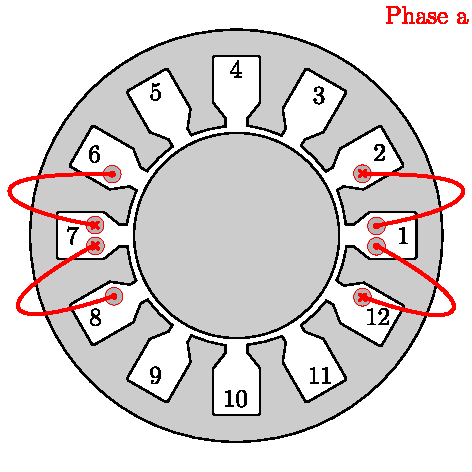
\includegraphics{ex04/MMF_concentrated.pdf}
    %\captionsetup{labelfont={color=blue},textfont={color=blue}}
    \caption{Simplified sketch of a concentrated winding. Only phase a is shown.}
    \label{fig:MMF_concentrated}
\end{figure}

%%%%%%%%%%%%%%%%%%%%%%%%%%%%%%%%%%%%%%%%%%%%%%%%%%%%%%%%%%%%%
\subtask{Determine the pole pitch and und the number of notches. Is it an integral-slot or a fractional-slot winding?}

\begin{solutionblock}
    The number of slots is determined by counting the slots in the given figure of the machine.
    Hence, the number of slots is $Q$ = 12. The number of phases is given in the task, which is $m$=3.
    Therefore, the pole pitch calculates as:
    \begin{equation}
        \rho_{\mathrm{p}} = \frac{2\pi}{2p}
        = \frac{\pi}{5}.
    \end{equation}

    The number of notches is determined with:
    \begin{equation}
        q = \frac{Q}{2pm}
        = \frac{12}{2 \cdot 5 \cdot 3}
        = \frac{2}{5}.
    \end{equation}
    Since the number of notches per pole and phase is not an integer, it is a fractional slot winding.
    The coil width $y$ is one stator slot, as it is shown in the figure. This results in the angular coil width: 
    \begin{equation}
        w = \frac{2\pi}{Q}
        = \frac{2\pi}{12}
        = \frac{\pi}{6}.
    \end{equation}

    Hence, the chording factor is calculated by:
    \begin{equation}
        s = \frac{w}{\tau_{\mathrm{p}}}
        = \frac{\pi \cdot 5}{6\pi}
        = \frac{5}{6}.
    \end{equation}

\end{solutionblock}

%%%%%%%%%%%%%%%%%%%%%%%%%%%%%%%%%%%%%%%%%%%%%%%%%%%%%%%%%%%%%
\subtask{Complete \autoref{tab:concentrated_winding} with the winding scheme for phases b and c. Sketch the resulting winding scheme in \autoref{fig:MMF_concentrated}.}

\begin{table}[ht]
    \caption{Winding scheme of a concentrated winding from \autoref{fig:MMF_concentrated}.}
    \centering
    \begin{tabular}{c|C{1cm}|C{1cm}|C{1cm}|C{1cm}|C{1cm}|C{1cm}}\toprule
        \multirow{2}{*}{Coil nr.} & \multicolumn{2}{c}{Phase a} & \multicolumn{2}{c}{Phase b} & \multicolumn{2}{c}{Phase c} \\
          & In  & Out   & In & Out & In & Out \\
        \midrule
        1  & 1  & 2  & & & & \\
        2  & 1  & 12  & & & & \\
        3  & 7  & 6  & & & & \\
        4  & 7  & 8  & & & & \\
        \bottomrule
    \end{tabular}
    \label{tab:concentrated_winding}
\end{table}


\begin{solutionblock}
    In the task only phase a of the winding scheme is given. However, to complete the winding scheme, phase b must have an electrical phase shift of $\SI{120}{\degree}$ and phase c of $\SI{240}{\degree}$ respectively.
    This leads to
    \begin{equation}
        n_{\mathrm{b}} p \frac{\SI{360}{\degree}}{Q} = \SI{120}{\degree} \ \mathrm{mod} \ \SI{360}{\degree},
    \end{equation}
    where $n_{\mathrm{b}}$ is the displacement in slots. This expression is rewritten into
    \begin{equation}
        n_{\mathrm{b}} p \frac{\SI{360}{\degree}}{Q} = \SI{120}{\degree} + k \SI{360}{\degree},
        \label{eq:nb_concentrated}
    \end{equation}
    and also for phase c:
    \begin{equation}
        n_{\mathrm{c}} p \frac{\SI{360}{\degree}}{Q} = \SI{240}{\degree} + k \SI{360}{\degree}.
        \label{eq:nc_concentrated}
    \end{equation}
    
    Now, an integral solution must be found for \eqref{eq:nb_concentrated} and \eqref{eq:nc_concentrated} to determine the winding scheme.
    This is done with trial and error, the first assumption is $n_{\mathrm{b}} = 8, k = 3$, which results in
    \begin{align}
        \begin{split}
            8\cdot 5\cdot \frac{\SI{360}{\degree}}{12} &= \SI{120}{\degree}+3 \cdot \SI{360}{\degree}, \\
            \SI{1200}{\degree} &= \SI{1200}{\degree},
        \end{split}
    \end{align}
    therefore, the requirement is fulfilled. For phase c the assumption is given with $n_{\mathrm{c}} = 4, k = 1$ into \eqref{eq:nc_concentrated} leads to
    \begin{align}
        \begin{split}
            4 \cdot 5 \cdot \frac{\SI{360}{\degree}}{12} &= \SI{240}{\degree} + k \SI{360}{\degree}, \\
            \SI{600}{\degree} &= \SI{600}{\degree},
        \end{split}
    \end{align}
    which fulfills the requirement too.

    With the coil width of one slot, the resulting winding is determined. The solution of this winding scheme is shown in \autoref{tab:solution_concentratedWinding}.
    \begin{solutiontable}[ht]
        \caption{Solution of the winding scheme of a concentrated winding.}
        \centering
        \begin{tabular}{c|C{1cm}|C{1cm}|C{1cm}|C{1cm}|C{1cm}|C{1cm}}\toprule
            \multirow{2}{*}{Coil nr.} & \multicolumn{2}{c}{Phase a} & \multicolumn{2}{c}{Phase b} & \multicolumn{2}{c}{Phase c} \\
              & In  & Out   & In & Out & In & Out \\
            \midrule
            1  & 1  & 2  & 3 & 2 & 4 & 5 \\
            2  & 1 & 12  & 3 & 4 & 6 & 5 \\
            3  & 7  & 6  & 8 & 9 & 11 & 10 \\
            4  & 7  & 8  & 10 & 9 & 11 & 12\\
            \bottomrule
        \end{tabular}
        \label{tab:solution_concentratedWinding}
    \end{solutiontable}
    

    The completed winding scheme is visualized in Fig.\ref{fig:solution_MMF_concentrated}.
    \begin{solutionfigure}[ht]
        \centering
        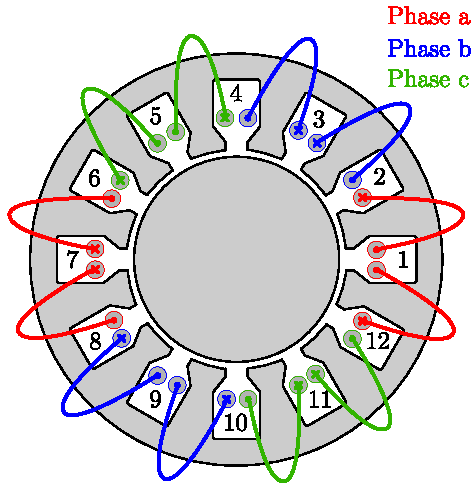
\includegraphics{ex04/solution_MMF_concentrated.pdf}
        \captionsetup{labelfont={color=blue},textfont={color=blue}}
        \caption{Solution of the concentrated winding scheme.}
        \label{fig:solution_MMF_concentrated}
    \end{solutionfigure}
\end{solutionblock}



%%%%%%%%%%%%%%%%%%%%%%%%%%%%%%%%%%%%%%%%%%%%%%%%%%%%%%%%%%%%%
\subtask{How many layers are in this winding scheme?}

\begin{solutionblock}
    There are two layers per slot, therefore, it is a two layer winding scheme.
\end{solutionblock}

%%%%%%%%%%%%%%%%%%%%%%%%%%%%%%%%%%%%%%%%%%%%%%%%%%%%%%%%%%%%%
\subtask{Calculate the complex winding factors $\underline{\xi}_{\mathrm{a,}k}$ for the fundamental as well as for the $5\textsuperscript{th}$ and $7\textsuperscript{th}$ harmonic.}

\begin{solutionblock}
    The complex winding factor is defined by
    \begin{equation}
        \underline{\xi}_{\mathrm{a,}k} = \frac{1}{\mathrm{j}N_{\mathrm{a}}} \sum_{i=1}^{Q} N_{\mathrm{a,}i}e^{\mathrm{j}k\vartheta_{\mathrm{el,a,}i}},
        \label{eq:complexWindingFactor_concentratedWinding}
    \end{equation}
    with
    \begin{equation}
        N_{\mathrm{a}} = \sum_{i=1}^{Q} |N_{\mathrm{a,}i} |,
    \end{equation}
    and the electrical angle:
    \begin{equation}
        \vartheta_{\mathrm{el,a,}i} = \vartheta_{\mathrm{a,}i} \cdot p.
    \end{equation}
    
    Hence, the mechanical angles are calculated as follows
    \begin{equation}
        \vartheta_{\mathrm{a,}i} = \left(i-1 \right) \frac{\SI{360}{\degree}}{Q}
        = \left(i-1 \right) \cdot \frac{\SI{360}{\degree}}{12}
        = \left(i-1 \right)\cdot \SI{30}{\degree},
    \end{equation}
    where $i$ represents the number of the stator slot.
    Therefore, the mechanical angles are given in \autoref{tab:mechanicalAngles_concentratedWinding}.
    \begin{solutiontable}[ht]
        \caption{Mechanical angles of the concentrated winding from \autoref{fig:MMF_concentrated}.}
        \centering
        \begin{tabular}{C{3cm}|C{3cm}}\toprule
            $\vartheta_{\mathrm{a,}1} = \SI{0}{\degree}$     & $\vartheta_{\mathrm{a,}9} = \SI{180}{\degree}$ \\
            $\vartheta_{\mathrm{a,}4} = \SI{30}{\degree}$    & $\vartheta_{\mathrm{a,}11} = \SI{210}{\degree}$ \\
            $\vartheta_{\mathrm{a,}5} = \SI{150}{\degree}$    & $\vartheta_{\mathrm{a,}12} = \SI{330}{\degree}$ \\
            \bottomrule
        \end{tabular}
        \label{tab:mechanicalAngles_concentratedWinding}
    \end{solutiontable}

    To calculate the winding factors, the total number of turns of the respective phase $N_{\mathrm{a}}$ is determined for each stator slot. A negative sign indicates, that the winding turn is oriented towards the negative $z$-axis. When no conductor is in a slot, $N_{\mathrm{a,}i}$ = 0. The result is shown in \autoref{tab:WindingTurns_concentratedWinding}.
    \begin{solutiontable}[ht]
        \caption{Winding turns of phase a of the concentrated winding rom \autoref{fig:MMF_concentrated}.}
        \centering
        \begin{tabular}{C{3cm}C{3cm}C{3cm}}\toprule
            $N_{\mathrm{a1}}$ = 2     & $N_{\mathrm{a2}}$ = -1  & $N_{\mathrm{a6}}$ = 1 \\
            $N_{\mathrm{a7}}$ = -2    & $N_{\mathrm{a8}}$ = 1   & $N_{\mathrm{a12}}$ = -1\\
            \bottomrule
        \end{tabular}
        \label{tab:WindingTurns_concentratedWinding}
    \end{solutiontable}
    
    For the fundamental wave, is $k$ = 1 and, therefore, with \eqref{eq:complexWindingFactor_concentratedWinding}, the winding factor of the fundamental wave calculates as follows:
    \begin{equation}
        \underline{\xi}_{\mathrm{a,}1} = \frac{1}{8j}\cdot \left[ \right. 2e^{j\cdot1\cdot5\cdot\SI{0}{\degree}}
        -e^{j\cdot1\cdot5\cdot\SI{30}{\degree}}+e^{j\cdot1\cdot5\cdot\SI{150}{\degree}}-2e^{j\cdot1\cdot5\cdot\SI{180}{\degree}}+e^{j\cdot1\cdot5\cdot\SI{210}{\degree}}
        -e^{j\cdot1\cdot5\cdot\SI{330}{\degree}}
        \left. \right]
        = -0.9330j,
    \end{equation}
    with the absolute value:
    \begin{equation}
        |\xi_{\mathrm{a,}1}| = 0.9330.
    \end{equation}

    For the $5\textsuperscript{th}$ harmonic is $k$ = 5, which results in
    \begin{equation}
        \underline{\xi}_{\mathrm{a,}5} = \frac{1}{8j}\cdot \left[ \right. 2e^{j\cdot5\cdot5\cdot\SI{0}{\degree}}
        -e^{j\cdot5\cdot5\cdot\SI{30}{\degree}}+e^{j\cdot5\cdot5\cdot\SI{150}{\degree}}-2e^{j\cdot5\cdot5\cdot\SI{180}{\degree}}+e^{j\cdot5\cdot5\cdot\SI{210}{\degree}}
        -e^{j\cdot5\cdot5\cdot\SI{330}{\degree}}
        \left. \right]
        = -0.067j,
    \end{equation}
    with the absolute value:
    \begin{equation}
        |\xi_{\mathrm{a,}5}| = 0.067.
    \end{equation}

    Finally, the complex winding factor for the $7\textsuperscript{th}$ harmonic is defined as
    \begin{equation}
        |\xi_{\mathrm{a,}7}| = \frac{1}{8j}\cdot \left[ \right. 2e^{j\cdot7\cdot5\cdot\SI{0}{\degree}}
        -e^{j\cdot7\cdot5\cdot\SI{30}{\degree}}+e^{j\cdot7\cdot5\cdot\SI{150}{\degree}}-2e^{j\cdot7\cdot5\cdot\SI{180}{\degree}}+e^{j\cdot7\cdot5\cdot\SI{210}{\degree}}
        -e^{j\cdot7\cdot5\cdot\SI{330}{\degree}}
        \left. \right]
        = -0.067j,
    \end{equation}
    and, therefore, the absolute value results in:
    \begin{equation}
        |\xi_{\mathrm{a,}7}| = 0.067.
    \end{equation}

\end{solutionblock}


%%%%%%%%%%%%%%%%%%%%%%%%%%%%%%%%%%%%%%%%%%%%%%%%%%%%%%%%%%%%%
\subtask{Assume a block-shaped distribution of the flux density with a maximal value of $\hat{B} = \SI{1}{\tesla}$ and a number of winding turns $N'_{\mathrm{a}}$ = 137. The axial length of the machine is $l=\SI{0.70}{\metre}$ and the diameter is $d = \SI{0.45}{\metre}$. The machine rotates with a mechanical speed of $n=\SI{50}{\per \minute}$. Calculate the induced voltage of phase a for the fundamental wave. What are the $5\textsuperscript{th}$ and $7\textsuperscript{th}$ harmonics of the induced voltage in phase a?}

\begin{solutionblock}
    The Fourier coefficient of the flux density is given with
    \begin{equation}
        B(\vartheta_{\mathrm{el}},t) = \frac{6}{\pi p} \hat{B} \sum_{k}^{\infty} \frac{1}{k} \sin\left(\frac{k\pi}{2} \right) \cos(\omega t - k \vartheta_{\mathrm{el}}),
    \end{equation}
    and for the fundamental wave:
    \begin{equation}
        B^{(1)}(\vartheta_{\mathrm{el}},t) = \frac{6}{\pi p} \hat{B} \sin\left(\frac{\pi}{2}\right) \cos(\omega t - \vartheta_{\mathrm{el}}).
    \end{equation}

    The flux linkage of phase a is calculated as
    \begin{equation}
        \phi_{\mathrm{a,}k}(t) = l \frac{d_{\mathrm{s}}}{2} |\xi_{\mathrm{a},k}| \int_{-\frac{\pi}{2}}^{\frac{\pi}{2}} B(\vartheta_{\mathrm{el}},t) \mathrm{d}\vartheta_{\mathrm{el}},
        \label{eq:phi_a_k_concentrated}
    \end{equation}
    with the complex winding factor to cover the winding distribution inside the stator.
    Hence, the fundamental wave calculates as follows:
    \begin{align}
        \begin{split}
            \phi_{\mathrm{a,}1}(t) &= l \frac{d_{\mathrm{s}}}{2} |\xi_{\mathrm{a},1}|
            \frac{6}{\pi p} \hat{B} \sin\left(\frac{\pi}{2}\right) \int_{-\frac{\pi}{2}}^{\frac{\pi}{2}} \cos(\omega t - \vartheta_{\mathrm{el}}) \mathrm{d}\vartheta_{\mathrm{el}} \\
            &= l d_{\mathrm{s}} |\xi_{\mathrm{a},1}|
            \frac{3}{\pi p} \hat{B}
            \int_{-\frac{\pi}{2}}^{\frac{\pi}{2}}\cos(\omega t) \cos(\vartheta_{\mathrm{el}}) + \sin(\omega t) \sin(\vartheta_{\mathrm{el}}) \mathrm{d}\vartheta_{\mathrm{el}} \\
            &= l d_{\mathrm{s}} |\xi_{\mathrm{a},1}|
            \frac{3}{\pi p} \hat{B}
            \left[\cos(\omega t) \int_{-\frac{\pi}{2}}^{\frac{\pi}{2}} \cos(\vartheta_{\mathrm{el}}) \mathrm{d}\vartheta_{\mathrm{el}} + \sin(\omega t) \int_{-\frac{\pi}{2}}^{\frac{\pi}{2}} \sin(\vartheta_{\mathrm{el}}) \mathrm{d} \vartheta_{\mathrm{el}} \right] \\
            &= l d_{\mathrm{s}} |\xi_{\mathrm{a},1}|
            \frac{3}{\pi p} \hat{B}
            \left[\cos(\omega t) \left[\sin(\vartheta_{\mathrm{el}}) \right]_{-\frac{\pi}{2}}^{\frac{\pi}{2}} + \sin(\omega t) \left[-\cos(\vartheta_{\mathrm{el}}) \right]_{-\frac{\pi}{2}}^{\frac{\pi}{2}} \right] \\
            &= l d_{\mathrm{s}} |\xi_{\mathrm{a},1}|
            \frac{3}{\pi p} \hat{B} \left[ 2 \cos(\omega t)\right] \\
            &= l d_{\mathrm{s}} |\xi_{\mathrm{a},1}|
            \frac{6}{\pi p} \hat{B} \cos(\omega t). \\
        \end{split}
    \end{align}

   Taking into account also the number of winding turns $N_{\mathrm{a}}'$, the flux linkage of phase a is given with 
    \begin{equation}
        \psi_{\mathrm{a,}k}(t) = N_{\mathrm{a}}' \phi_{\mathrm{a,}k}(t),
        \label{eq:psi_a_k_concentrated}
    \end{equation}
    which results for the fundamental wave into:
    \begin{align}
        \begin{split}
            \psi_{\mathrm{a,}1}(t) &= N_{\mathrm{a}}' \phi_{\mathrm{a,}k}(t) 
            = N_{\mathrm{a}}' l d_{\mathrm{s}} |\xi_{\mathrm{a},1}| \frac{6}{\pi p} \hat{B} \cos(\omega t) \\
            &= 137 \cdot \SI{0.7}{\metre} \cdot \SI{0.45}{\metre} \cdot \frac{6}{5\pi} \cdot \SI{1}{\tesla} \cos(\omega t) \cdot 0.9330 \\
            &= \SI{15.38}{\volt\second} \cdot \cos(\omega t).
        \end{split}
    \end{align}

    The equation for the induced voltage of the fundamental wave is given with:
    \begin{align}
        \begin{split}
            u_{\mathrm{ind,a,}1}(t) &= -\frac{\mathrm{d}}{\mathrm{d}t}\psi_{\mathrm{a,}1} \\
            &= -\frac{\mathrm{d}}{\mathrm{d}t} \SI{15.38}{\volt\second} \cdot \cos(\omega t) \\
            &= \SI{15.38}{\volt\second} \cdot \sin(\omega t) \omega \\
            &= \SI{15.38}{\volt\second} \cdot \sin(\omega t) \cdot 2\pi \cdot 5 \cdot \SI{\frac{50}{60}}{\per\second} \\
            &= \SI{402.6}{\volt} \cdot \sin(\omega t).
        \end{split}
    \end{align}

    The flux linkage of the $5\textsuperscript{th}$ harmonic is determined with \eqref{eq:phi_a_k_concentrated}, which results into:
    \begin{align}
        \begin{split}
            \phi_{\mathrm{a,}5}(t) &= l \frac{d_{\mathrm{s}}}{2} |\xi_{\mathrm{a},5}|
            \frac{6}{\pi p} \hat{B}\frac{1}{5} \sin\left(\frac{5\pi}{2}\right) \int_{-\frac{\pi}{2}}^{\frac{\pi}{2}} \cos(\omega t - 5\vartheta_{\mathrm{el}}) \mathrm{d}\vartheta_{\mathrm{el}} \\
            &  \vdots \\
            &= l \frac{d_{\mathrm{s}}}{2} |\xi_{\mathrm{a},5}|
            \frac{6}{\pi p} \hat{B} \frac{1}{5} \cos(\omega t).
        \end{split}
    \end{align}
    The resulting flux linkage is calculated by taking into account the number of winding turns as
    \begin{align}
        \begin{split}
            \psi_{\mathrm{a,}5} &= N_{\mathrm{a}}' \phi_{\mathrm{a,}5}(t) 
            = N_{\mathrm{a}}' l \frac{d_{\mathrm{s}}}{2} |\xi_{\mathrm{a},5}| \frac{6}{\pi p} \hat{B} \frac{1}{5} \cos(\omega t) \\
            &= 137 \cdot \SI{0.7}{\metre} \cdot \SI{\frac{0.45}{2}}{\metre} \cdot \frac{6}{5\pi} \cdot \SI{1}{\tesla} \cdot \frac{1}{5} \cdot \cos(\omega t) \cdot 0.0067 \\
            &= \SI{0.2208}{\volt\second} \cdot \cos(\omega t),
        \end{split}
    \end{align}
    therefore, the induced voltage is given with:
    \begin{align}
        \begin{split}
            u_{\mathrm{ind,a,}5}(t) &= -\frac{\mathrm{d}}{\mathrm{d}t}\psi_{\mathrm{a,}5} \\
            &= \SI{0.2208}{\volt\second} \cdot \sin(\omega t) \omega \\
            &= \SI{0.2208}{\volt\second} \cdot \SI{2\pi\cdot 5\cdot \frac{50}{60}}{\per\second} \\
            &= \SI{5.78}{\volt} \cdot \sin(\omega t).
        \end{split}
    \end{align}
    

    With \eqref{eq:phi_a_k} the flux linkage for the $7\textsuperscript{th}$ harmonic is calculated by:
    \begin{align}
        \begin{split}
            \phi_{\mathrm{a,}7}(t) &= l \frac{d_{\mathrm{s}}}{2} |\xi_{\mathrm{a},7}|
            \frac{6}{\pi p} \hat{B}\frac{1}{7} \sin\left(\frac{7\pi}{2}\right) \int_{-\frac{\pi}{2}}^{\frac{\pi}{2}} \cos(\omega t - 7\vartheta_{\mathrm{el}}) \mathrm{d}\vartheta_{\mathrm{el}} \\
            &  \vdots \\
            &= l \frac{d_{\mathrm{s}}}{2} |\xi_{\mathrm{a},7}|
            \frac{6}{\pi p} \hat{B} \frac{1}{7} \cos(\omega t).
        \end{split}
    \end{align}

    The resulting flux linkage is calculated by taking into account the number of winding turns as
    \begin{align}
        \begin{split}
            \psi_{\mathrm{a,}7} &= N_{\mathrm{a}}' \phi_{\mathrm{a,}7}(t) 
            = N_{\mathrm{a}}' l \frac{d_{\mathrm{s}}}{2} |\xi_{\mathrm{a},7}| \frac{6}{\pi p} \hat{B} \frac{1}{7} \cos(\omega t) \\
            &= 137 \cdot \SI{0.7}{\metre} \cdot \SI{\frac{45}{2}}{\metre} \cdot \frac{6}{5\pi} \cdot \SI{1}{\tesla} \cdot \frac{1}{7} \cdot \cos(\omega t) \cdot 0.067 \\
            &= \SI{0.0156}{\volt\second} \cdot \cos(\omega t),
        \end{split}
    \end{align}
    therefore, the induced voltage is given with:
    \begin{align}
        \begin{split}
            u_{\mathrm{ind,a,}7}(t) &= -\frac{\mathrm{d}}{\mathrm{d}t}\psi_{\mathrm{a,}7} \\
            &= \SI{0.0156}{\volt\second} \cdot \sin(\omega t) \omega \\
            &= \SI{0.0156}{\volt\second} \cdot \SI{2\pi\cdot 5\cdot \frac{50}{60}}{\per\second} \\
            &= \SI{4.13}{\volt}.
        \end{split}
    \end{align}

\end{solutionblock}


%%%%%%%%%%%%%%%%%%%%%%%%%%%%%%%%%%%%%%%%%%%%%%%%%%%%%%%%%%%%%
\subtask{Calcualte with a Python script the complex winding factor $\underline{\xi}_{\mathrm{a,}k}$ up to various harmonics.}

\begin{solutionblock}
    The Python script is separately available, therefore, only the solution is presented in Tab~\ref{tab:complexWindingFactor_concentratedW_python}.
    \begin{solutiontable}[ht]
        \caption{Complex winding factors $\underline{\xi}_{\mathrm{a,}k}$ for the concentrated winding up to the $12\textsuperscript{th}$ harmonic order.}
        \centering
        \begin{tabular}{R{3cm}R{3cm}R{3cm}R{3cm}}\toprule
            $\underline{\xi}_{\mathrm{a,}1}$ = -0.9330j    & $\underline{\xi}_{\mathrm{a,}2}$ = 0 &
            $\underline{\xi}_{\mathrm{a,}3}$ = -0.5j       & $\underline{\xi}_{\mathrm{a,}4}$ = 0 \\
            $\underline{\xi}_{\mathrm{a,}5}$ = -0.0670j    & $\underline{\xi}_{\mathrm{a,}6}$ = 0 &
            $\underline{\xi}_{\mathrm{a,}7}$ = -0.0670j    & $\underline{\xi}_{\mathrm{a,}8}$ = 0 \\
            $\underline{\xi}_{\mathrm{a,}9}$ = -0.5j       & $\underline{\xi}_{\mathrm{a,}10}$ = 0 &
            $\underline{\xi}_{\mathrm{a,}11}$ = -0.9330j   & $\underline{\xi}_{\mathrm{a,}12}$ = 0 \\
            \bottomrule
        \end{tabular}
        \label{tab:complexWindingFactor_concentratedW_python}
    \end{solutiontable}

    %It should be mentioned, that only harmonics of $k = 
\end{solutionblock}

    %%%%%%%%%%%%%%%%%%%%%%%%%%%%%%%%%%%%%%%%%%%%%%%%%%%%%%%%%%%%%
%% Begin exercise %%
%%%%%%%%%%%%%%%%%%%%%%%%%%%%%%%%%%%%%%%%%%%%%%%%%%%%%%%%%%%%%
\ex{Transient and steady state of an induction machine}


\normalsize{\textbf{Acknowledgement}: The following exercise is adapted from ``Geregelte Drehstromantriebe / Controlled AC Drives'' by J. Böcker, Paderborn University, 2021
}\\




%%%%%%%%%%%%%%%%%%%%%%%%%%%%%%%%%%%%%%%%%%%%%%%%%%%%%%%%%%%%%
%% Task 1 %%
%%%%%%%%%%%%%%%%%%%%%%%%%%%%%%%%%%%%%%%%%%%%%%%%%%%%%%%%%%%%%

\task{Transient simulation of an induction machine}
Given is a squirrel cage motor with the characteristics in Tab.~\ref{tab:characteristicsIM}. The motor is operated with the stator frequency $f_{\mathrm{s}}$ = 50 Hz and a line-to-line voltage of $U_{\mathrm{ll}}$ = 400 V, that is, connected to grid.

\begin{table}[htb]
    \caption{Characteristics of the induction machine.}
    \centering
    \begin{tabular}{lll}\toprule
    Symbol  & Description       & Value \\
    \midrule
    $T_{\mathrm{n}}$    & Nominal torque            & $\SI{4.7}{\newton\metre}$ \\
    $I_{\mathrm{n}}$    & Nominal phase current     & $\SI{3.9}{\ampere}$ \\
    $P_{\mathrm{n}}$    & Nominal power             & $\SI{1.5}{\kilo\watt}$ \\
    $n_{\mathrm{n}}$    & Nominal speed             & $\SI{3000}{\per\minute}$ \\
    \bottomrule
    \end{tabular}
    \label{tab:characteristicsIM}
\end{table}


%%%%%%%%%%%%%%%%%%%%%%%%%%%%%%%%%%%%%%%%%%%%%%%%%%%%%%%%%%%%%
\subtask{Determine the equations of the induction machine in the rotor flux oriented coordinate system. Therefore, only the stator current $i_{\mathrm{s,dq}}(t)$ and the rotor flux $\psi_{\mathrm{r,d}}(t)$ should occur as state variables.}

\begin{solutionblock}
    The stator equations in the k coordinate system from the lecture are defined by:
    \begin{equation}
        \frac{\mathrm{d}}{\mathrm{d}t} \psi_{\mathrm{s,d}}^{\mathrm{k}}(t) = \omega_{\mathrm{k,el}} \psi_{\mathrm{s,q}}^{\mathrm{k}}(t) + u_{\mathrm{s,d}}^{\mathrm{k}}(t) - R_{\mathrm{s}} i_{\mathrm{s,d}}^{\mathrm{k}}(t),
        \label{eq:ode_stator_d}
    \end{equation}

    \begin{equation}
        \frac{\mathrm{d}}{\mathrm{d}t} \psi_{\mathrm{s,q}}^{\mathrm{k}}(t) = - \omega_{\mathrm{k,el}} \psi_{\mathrm{s,d}}^{\mathrm{k}}(t) + u_{\mathrm{s,q}}^{\mathrm{k}}(t) - R_{\mathrm{s}} i_{\mathrm{s,q}}^{\mathrm{k}}(t).
    \end{equation}


    The rotor equations in the k coordinate system are defined as: 
    \begin{equation}
        \frac{\mathrm{d}}{\mathrm{d}t} \psi_{\mathrm{r,d}}^{\mathrm{k}}(t) = (\omega_{\mathrm{k,el}}(t)-\omega_{\mathrm{r,el}}(t))\psi_{\mathrm{r,q}}^{\mathrm{k}}(t) + u_{\mathrm{r,d}}^{\mathrm{k}}(t) - R_{\mathrm{r}}i_{\mathrm{r,d}}^{\mathrm{k}}(t),
        \label{eq:ode_rotor_d}
    \end{equation}

    \begin{equation}
        \frac{\mathrm{d}}{\mathrm{d}t} \psi_{\mathrm{r,q}}^{\mathrm{k}}(t) = -(\omega_{\mathrm{k,el}}(t)-\omega_{\mathrm{r,el}}(t))\psi_{\mathrm{r,d}}^{\mathrm{k}}(t) + u_{\mathrm{r,q}}^{\mathrm{k}}(t) - R_{\mathrm{r}}i_{\mathrm{r,q}}^{\mathrm{k}}(t).
    \end{equation}
    
    For the further consideration, only the stator current and the rotor flux are of interest as state variables. Therefore, the rotor current and stator flux are being eliminated with the help of the following equations
    \begin{align}
        \begin{split}
            i_{\mathrm{r,d}}(t) &= \frac{1}{L_{\mathrm{r}}} \psi_{\mathrm{r,d}}(t) - \frac{M_{\mathrm{r}}}{L_{\mathrm{r}}}i_{\mathrm{s,d}}(t), \\
            i_{\mathrm{r,q}}(t) &= \frac{1}{L_{\mathrm{r}}} \psi_{\mathrm{r,q}}(t) - \frac{M_{\mathrm{r}}}{L_{\mathrm{r}}}i_{\mathrm{s,q}}(t), \\
        \end{split}
        \label{eq:rotorCurrent}
    \end{align}
    and:
    \begin{align}
        \begin{split}
            \psi_{\mathrm{s,d}}(t) &= \sigma L_{\mathrm{s}} i_{\mathrm{s,d}}(t) + \frac{M_{\mathrm{s}}}{L_{\mathrm{r}}} \psi_{\mathrm{r,d}}(t), \\
            \psi_{\mathrm{s,q}}(t) &= \sigma L_{\mathrm{s}} i_{\mathrm{s,q}}(t) + \frac{M_{\mathrm{s}}}{L_{\mathrm{r}}} \psi_{\mathrm{r,q}}(t). \\
        \end{split}
        \label{eq:statorFlux}
    \end{align}
    These equations are derived from the magnetic circuit of the induction machine.


    The rotor current from \eqref{eq:rotorCurrent} is inserted in the rotor equation \eqref{eq:ode_rotor_d}. In addition, the coordinate system is aligned with the rotor flux.
    This results in the following equation for the d-axis:
    \begin{equation}
        \frac{\mathrm{d}}{\mathrm{d}t} \psi_{\mathrm{r,d}}(t) = (\omega_{\mathrm{k,el}}(t)-\omega_{\mathrm{r,el}}(t))\psi_{\mathrm{r,q}}(t) + u_{\mathrm{r,d}}(t) - R_{\mathrm{r}} \left(\frac{1}{L_{\mathrm{r}}} \psi_{\mathrm{r,d}}(t) - \frac{M_{\mathrm{r}}}{L_{\mathrm{r}}}i_{\mathrm{s,d}}(t) \right).
    \end{equation}
    
    Within the rotor flux-oriented coordinate system, only a flux in d-axis occurs, therefore, the equation can be simplified into
    \begin{equation}
        \frac{\mathrm{d}}{\mathrm{d}t}\psi_{\mathrm{r,d}} = u_{\mathrm{r,d}}(t) - \frac{R_{\mathrm{r}}}{L_{\mathrm{r}}} \psi_{\mathrm{r,d}}(t) + \frac{R_{\mathrm{r}}M_{\mathrm{r}}}{L_{\mathrm{r}}}i_{\mathrm{s,d}}(t),
    \end{equation}
    and due to the squirrel cage machine the rotor voltage is zero. This leads to:
    \begin{equation}
        \frac{\mathrm{d}}{\mathrm{d}t}\psi_{\mathrm{r,d}} = - \frac{R_{\mathrm{r}}}{L_{\mathrm{r}}} \psi_{\mathrm{r,d}}(t) + \frac{R_{\mathrm{r}}M_{\mathrm{r}}}{L_{\mathrm{r}}}i_{\mathrm{s,d}}(t).
    \end{equation}

    For the q-axis, the rotor current form \eqref{eq:rotorCurrent} is also used in the rotor flux differential equation. This leads to:
    \begin{equation}
        \frac{\mathrm{d}}{\mathrm{d}t} \psi_{\mathrm{r,q}}(t) = -(\omega_{\mathrm{k,el}}(t)-\omega_{\mathrm{r,el}}(t))\psi_{\mathrm{r,d}}(t) + u_{\mathrm{r,q}}(t) - R_{\mathrm{r}} \left(\frac{1}{L_{\mathrm{r}}} \psi_{\mathrm{r,q}}(t) - \frac{M_{\mathrm{r}}}{L_{\mathrm{r}}}i_{\mathrm{s,q}}(t) \right),
    \end{equation}
    and with the definition for $\psi_{\mathrm{r,q}}(t)$ = 0:
    \begin{equation}
        \frac{\mathrm{d}}{\mathrm{d}t} \psi_{\mathrm{r,q}}(t) = 0 = -(\omega_{\mathrm{k,el}}(t)-\omega_{\mathrm{r,el}}(t))\psi_{\mathrm{r,d}}(t) + u_{\mathrm{r,q}}(t) + R_{\mathrm{r}} \frac{M_{\mathrm{r}}}{L_{\mathrm{r}}}i_{\mathrm{s,q}}(t).
    \end{equation}
    Due to the squirrel cage motor type, the rotor voltage is zero. However, the slip frequency is determined from this equation as follows:
    \begin{equation}
        -(\omega_{\mathrm{k,el}}(t)-\omega_{\mathrm{r,el}}(t))
        = R_{\mathrm{r}} \frac{M_{\mathrm{r}}}{L_{\mathrm{r}}} \frac{i_{\mathrm{s,q}}(t)}{\psi_{\mathrm{r,d}}(t)}.
    \end{equation}

    In the next step, the stator flux is eliminated in \eqref{eq:ode_stator_d}. Therefore, \eqref{eq:statorFlux}  is used as follows
    \begin{equation}
        \sigma L_{\mathrm{s}} \frac{\mathrm{d}}{\mathrm{d}t} i_{\mathrm{s,d}}(t) + \frac{M_{\mathrm{s}}}{L_{\mathrm{r}}} \frac{\mathrm{d}}{\mathrm{d}t}\psi_{\mathrm{r,d}}(t) = \omega_{\mathrm{k,el}}(t) \left(\sigma L_{\mathrm{s}} i_{\mathrm{s,q}}(t) + \frac{M_{\mathrm{s}}}{L_{\mathrm{r}}} \psi_{\mathrm{r,q}}(t) \right) + u_{\mathrm{s,d}}(t) - R_{\mathrm{s}} i_{\mathrm{s,d}}(t),
    \end{equation}
    with the derivative of the previous determined rotor flux
    \begin{equation}
        \sigma L_{\mathrm{s}} \frac{\mathrm{d}}{\mathrm{d}t} i_{\mathrm{s,d}}(t) + \frac{M_{\mathrm{s}}}{L_{\mathrm{r}}} \left(u_{\mathrm{r,d}}(t) - \frac{R_{\mathrm{r}}}{L_{\mathrm{r}}} \psi_{\mathrm{r,d}}(t) + \frac{R_{\mathrm{r}}M_{\mathrm{r}}}{L_{\mathrm{r}}}i_{\mathrm{s,d}}(t) \right)
        =
        \omega_{\mathrm{k,el}} \sigma L_{\mathrm{s}} i_{\mathrm{s,q}}(t) + u_{\mathrm{s,d}}(t) - R_{\mathrm{s}} i_{\mathrm{s,d}}(t),
    \end{equation}
    which leads to:
    \begin{align}
        \begin{split}
            \frac{\mathrm{d}}{\mathrm{d}t} i_{\mathrm{s,d}}(t) &= \frac{1}{\sigma L_{\mathrm{s}}}
            \left[ 
                -\frac{M_{\mathrm{s}}}{L_{\mathrm{r}}} u_{\mathrm{r,d}}(t) + \psi_{\mathrm{r,d}}(t) \frac{M_{\mathrm{s}}R_{\mathrm{r}}}{L_{\mathrm{r}}^{2}} \right.\\
                &+ \left. \omega_{\mathrm{k,el}}(t) \sigma L_{\mathrm{s}} i_{\mathrm{s,q}}(t) + u_{\mathrm{s,d}}(t) + i_{\mathrm{s,d}}(t) \left(-\frac{R_{\mathrm{r}}M_{\mathrm{s}}^2}{L_{\mathrm{r}}^2} - R_{\mathrm{s}} \right)
            \right].
        \end{split}
    \end{align}


    Again, eliminate the stator flux in the ode with \eqref{eq:statorFlux} for the q-axis, which leads to
    \begin{equation}
        \sigma L_{\mathrm{s}} \frac{\mathrm{d}}{\mathrm{d}t} i_{\mathrm{s,q}}(t) + \frac{M_{\mathrm{s}}}{L_{\mathrm{r}}} \frac{\mathrm{d}}{\mathrm{d}t} \psi_{\mathrm{r,q}}(t)
        =
        - \omega_{\mathrm{k,el}}(t) \psi_{\mathrm{s,d}}(t) + u_{\mathrm{s,q}}(t) - R_{\mathrm{s}} i_{\mathrm{s,q}}(t),
    \end{equation}

    with $\psi_{\mathrm{r,q}} = 0$ and the derivative $\frac{\mathrm{d}}{\mathrm{d}t}\psi_{\mathrm{r,q}} = 0$, the equation results in:
    \begin{equation}
        \sigma L_{\mathrm{s}} \frac{\mathrm{d}}{\mathrm{d}t} i_{\mathrm{s,q}}(t)
        =
        -\omega_{\mathrm{k,el}}(t)\psi_{\mathrm{s,d}}(t) + u_{\mathrm{s,q}}(t) - R_{\mathrm{s}} i_{\mathrm{r,q}}(t).
    \end{equation}

    Hence, the ODEs for the stator currents and the rotor flux are given in the following. It starts with the d-current component, which is given with:
    \begin{align}
        \begin{split}
            \frac{\mathrm{d}}{\mathrm{d}t} i_{\mathrm{s,d}}(t) &= \frac{1}{\sigma L_{\mathrm{s}}}
            \left[ 
                -\frac{M_{\mathrm{s}}}{L_{\mathrm{r}}} u_{\mathrm{r,d}}(t) + \psi_{\mathrm{r,d}}(t) \frac{M_{\mathrm{s}}R_{\mathrm{r}}}{L_{\mathrm{r}}^{2}} \right.\\
                &+ \left. \omega_{\mathrm{k,el}}(t) \sigma L_{\mathrm{s}} i_{\mathrm{s,q}}(t) + u_{\mathrm{s,d}}(t) + i_{\mathrm{s,d}}(t) \left(-\frac{R_{\mathrm{r}}M_{\mathrm{s}}^2}{L_{\mathrm{r}}^2} - R_{\mathrm{s}} \right)
            \right],
        \end{split}
    \end{align}
    for the stator q-current
    \begin{equation}
        \frac{\mathrm{d}}{\mathrm{d}t} i_{\mathrm{s,q}}(t) = \frac{1}{\sigma L_{\mathrm{s}}}
            \left[-\omega_{\mathrm{k,el}}(t)\psi_{\mathrm{s,d}}(t) + u_{\mathrm{s,q}}(t) - R_{\mathrm{s}} i_{\mathrm{r,q}}(t)\right],
    \end{equation}
    and the rotor flux in the d-axis:
    \begin{equation}
        \frac{\mathrm{d}}{\mathrm{d}t}\psi_{\mathrm{r,d}} = - \frac{R_{\mathrm{r}}}{L_{\mathrm{r}}} \psi_{\mathrm{r,d}}(t) + \frac{R_{\mathrm{r}}M_{\mathrm{r}}}{L_{\mathrm{r}}}i_{\mathrm{s,d}}(t).
    \end{equation}

    To simulate the induction machine, also the mechanical part must be taken into account. Hence, the mechanical equation is given by
    \begin{equation}
        J \frac{\mathrm{d}}{\mathrm{d}t}\omega_{\mathrm{r,el}}(t) = T(t) - T_{\mathrm{l}}(t),
    \end{equation}
    where $T(t)$ represents the produced torque and $T_{\mathrm{l}}(t)$ is the load torque. This leads to
    \begin{equation}
        \frac{\mathrm{d}}{\mathrm{d}t}\omega_{\mathrm{r,el}}(t) = \frac{1}{J}\left(T(t)-T_{\mathrm{l}}(t)\right),
    \end{equation}
    where $T(t)$ is defined as
    \begin{equation}
        T(t) = -\frac{3}{2} p \left(i_{\mathrm{r,dq}}^{\mathrm{k}}(t)\right)^{\top} \bm{J} \psi_{\mathrm{r,dq}}^{\mathrm{k}}(t),
    \end{equation}
    which results in the rotor oriented coordinate system into:
    \begin{equation}
        T(t) = \frac{3}{2} p \hspace{0.5mm} i_{\mathrm{r,d}}(t)\psi_{\mathrm{r,q}}(t) - \frac{3}{2} p \hspace{0.5mm} i_{\mathrm{r,q}}(t)\psi_{\mathrm{r,d}}(t).
    \end{equation}
    The first part from the equation above is zero, due to the definition of the coordinate system. The rotor current is replaced with \eqref{eq:rotorCurrent}, that leads to:
    \begin{align}
        \begin{split}
            T(t) &= -\frac{3}{2} p \left(\frac{1}{L_{\mathrm{r}}} \psi_{\mathrm{r,q}}(t) - \frac{M_{\mathrm{r}}}{L_{\mathrm{r}}} i_{\mathrm{s,q}}(t) \right) \psi_{\mathrm{r,d}}(t) \\
            &= \frac{3}{2} \frac{M_{\mathrm{r}}}{L_{\mathrm{r}}} i_{\mathrm{s,q}}(t) \psi_{\mathrm{r,d}}(t).
        \end{split}
    \end{align}


\end{solutionblock}

%%%%%%%%%%%%%%%%%%%%%%%%%%%%%%%%%%%%%%%%%%%%%%%%%%%%%%%%%%%%%
\subtask{Write a Jupyter notebook to solve the derived equations in the dq coordinate system aligned to the rotor flux from the previous task. First, simulate the machine with no load. Analyze the transient motor response starting from the initial state $i_{\mathrm{d}}(t=0)=i_{\mathrm{q}}(t=0)=\psi_{\mathrm{d}}(t=0)=\omega_{\mathrm{el}}(t=0)=\epsilon_{\mathrm{el}}(t=0)=0$ when excited with the above-mentioned stator voltage. Simulate as well as visualize the torque, speed, flux and current responses and plot the latter two in abc, $\upalpha\upbeta$ and dq coordinates.}

\begin{solutionblock}
    The current in the dq coordinate system is shown in \autoref{fig:i_dq_noLoad}. After the steady state is reached, the current values are constant, which could be expected in the rotor flux-oriented coordinate system.
    \begin{solutionfigure}[ht]
        \centering
        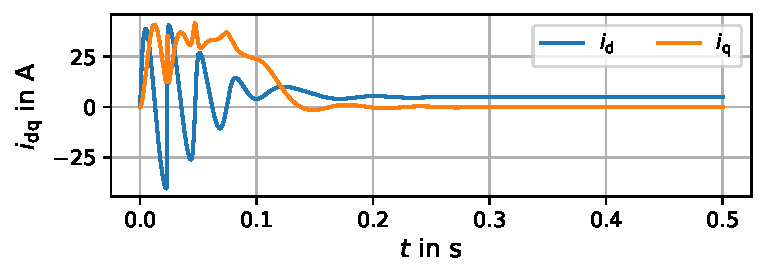
\includegraphics{ex05/i_dq_noLoad.pdf}
        \caption{Transient process of an IM in the dq coordinate system.}
        \label{fig:i_dq_noLoad}
    \end{solutionfigure}

    In \autoref{fig:i_ab_noLoad} the current in the $\upalpha, \upbeta$ coordinate system is visualized. The transient process is also clearly visible in this coordinate system.
    \begin{solutionfigure}[ht]
        \centering
        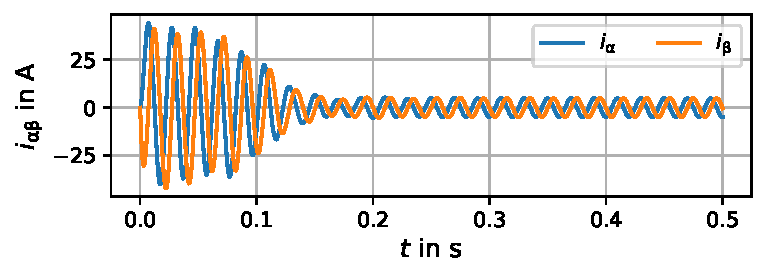
\includegraphics{ex05/i_alphaBeta_noLoad.pdf}
        \caption{Transient process of an IM in the $\upalpha \upbeta$ coordinate system.}
        \label{fig:i_ab_noLoad}
    \end{solutionfigure}

    \autoref{fig:i_abc_noLoad} shows the transient process of the current in the three-phase abc coordinate system.
    
    Compared to the abc current plot, one can observe also a sinusoidal signalform with the same amplitude and frequency evolution, while the phase difference between the currents is 120° in abc and 90° in $\upalpha\upbeta$. This fits to the expectations resulting from the amplitude-invariant Clarke transformation.
    \begin{solutionfigure}[ht]
        \centering
        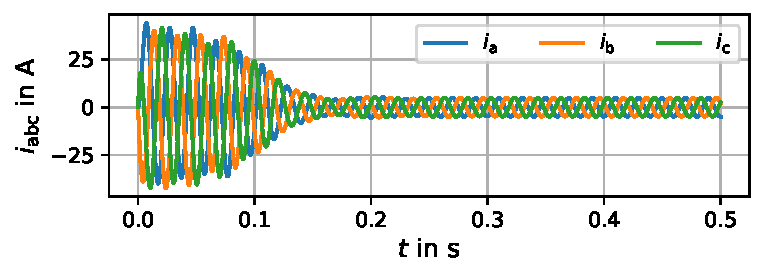
\includegraphics{ex05/i_abc_noLoad.pdf}
        \caption{Transient process of an IM in the abc coordinate system.}
        \label{fig:i_abc_noLoad}
    \end{solutionfigure}

    The electrical angular frequency of the stator and the angular frequency of the rotor are shown in \autoref{fig:speed_noLoad}. Due to the no load operation (also no friction) of the IM, the angular frequency of the rotor is equal to the angular electrical stator frequency.
    \begin{solutionfigure}[ht]
        \centering
        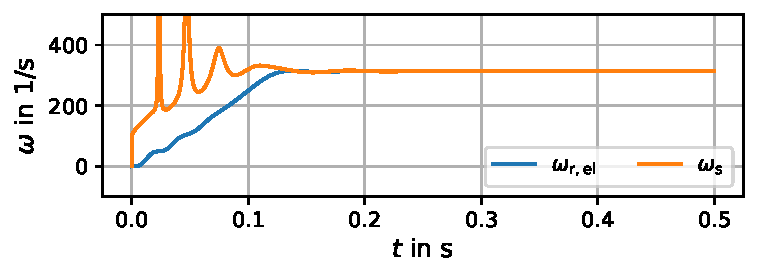
\includegraphics{ex05/speed_noLoad.pdf}
        \caption{Electric angular frequency of the stator and angular frequency of the rotor during the transient process at no load.}
        \label{fig:speed_noLoad}
    \end{solutionfigure}

    The produced torque is shown in \autoref{fig:torque_noLoad}. During the transient process, very high torque values are reached and an oscillation of the rotor is visible. In the steady state, the torque is equal to zero, due to the no-load operation.
    \begin{solutionfigure}[ht]
        \centering
        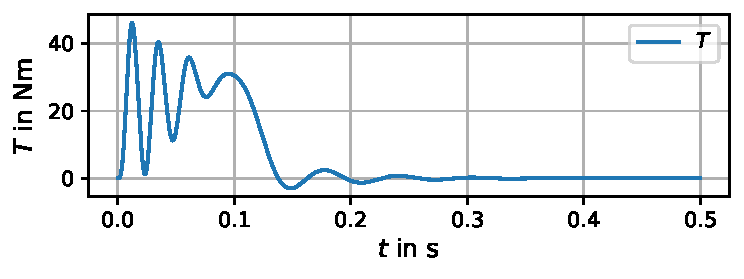
\includegraphics{ex05/torque_noLoad.pdf}
        \caption{Produced torque of an IM during the transient process at no load.}
        \label{fig:torque_noLoad}
    \end{solutionfigure}

    In \autoref{fig:rotorFlux_noLoad} the rotor flux is shown, which also shows the transient process. The d-axis of the coordinate system is oriented on the rotor flux and, therefore, the flux aligned to the q-axis is zero. Thus, only the rotor flux aligned to the d-axis is visualized.
    \begin{solutionfigure}[ht]
        \centering
        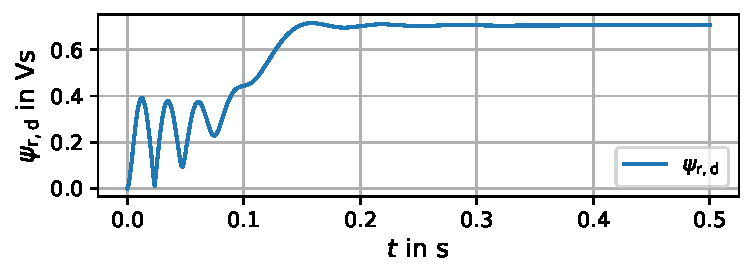
\includegraphics{ex05/psi_rd_noLoad.pdf}
        \caption{Rotor flux in dq coordinate system during the transient process at no load.}
        \label{fig:rotorFlux_noLoad}
    \end{solutionfigure}

    \begin{solutionfigure}[ht]
        \centering
        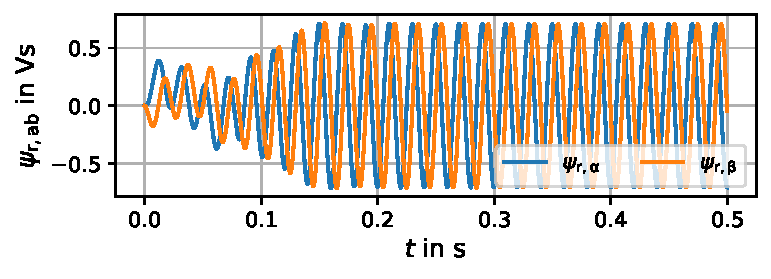
\includegraphics{ex05/psi_r_ab_noLoad.pdf}
        \caption{Rotor flux in $\upalpha\upbeta$ coordinate system during the transient process at no load.}
        \label{fig:rotorFlux_r_ab_noLoad}
    \end{solutionfigure}

    \begin{solutionfigure}[ht]
        \centering
        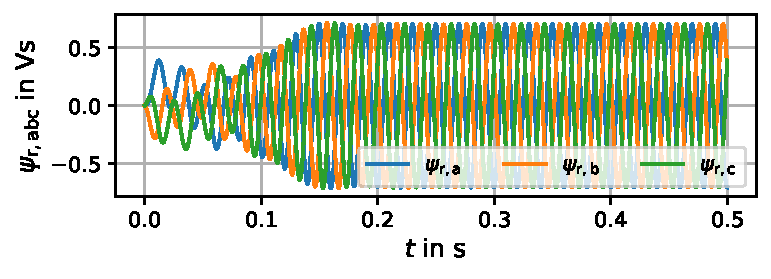
\includegraphics{ex05/psi_r_abc_noLoad.pdf}
        \caption{Rotor flux in abc coordinate system during the transient process at no load.}
        \label{fig:rotorFlux_r_abc_noLoad}
    \end{solutionfigure}

\end{solutionblock}


\FloatBarrier

%%%%%%%%%%%%%%%%%%%%%%%%%%%%%%%%%%%%%%%%%%%%%%%%%%%%%%%%%%%%%
\subtask{Add a speed dependent load with the following equation $T_{\mathrm{l}} = 0.00004*\omega_{\mathrm{r,el}}^2$ to the machine model. Repeat the simulation from the previous task. How does the currents, torque and flux change? In addition, how changes the rotational speed of the machine between these two operating points?}

\begin{solutionblock}
    In \autoref{fig:speed_friction} the speed of the stator and rotor field is visualized. For this simulation a load term representing the friction is added, thus this load is speed dependent. Hence, this results in a different speed of the rotor in the steady state in comparison to the stator field. This occurs due to the load of the machine, and is representing with the slip of the machine.
    \begin{solutionfigure}[ht]
        \centering
        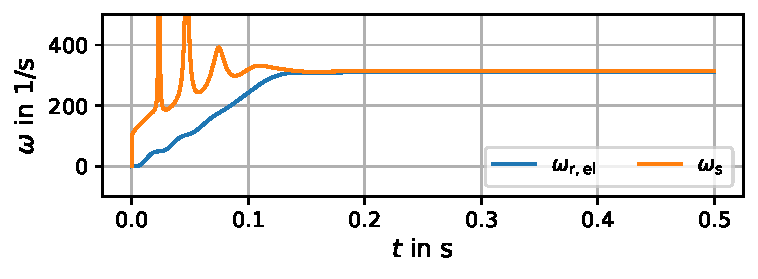
\includegraphics{ex05/speed_friction.pdf}
        \caption{Electrical angular frequency of the stator and angular frequency of the rotor during the transient process with a speed dependent load.}
        \label{fig:speed_friction}
    \end{solutionfigure}
    
    To highlight the difference between the stator and rotor field, in \autoref{fig:speed_zoom_friction} the boundaries of the vertical axis are limited. Hence, the speed difference in the steady state is clearly visible.
    \begin{solutionfigure}[ht]
        \centering
        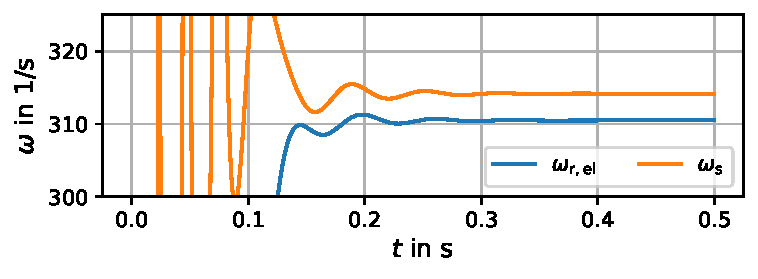
\includegraphics{ex05/speed_zoom_friction.pdf}
        \caption{Zoom into the electrical angular frequency of the stator and angular frequency of the rotor to visualize the difference in the steady state.}
        \label{fig:speed_zoom_friction}
    \end{solutionfigure}

    The produced torque during the transient process is shown in \autoref{fig:torque_friction}.
    \begin{solutionfigure}[ht]
        \centering
        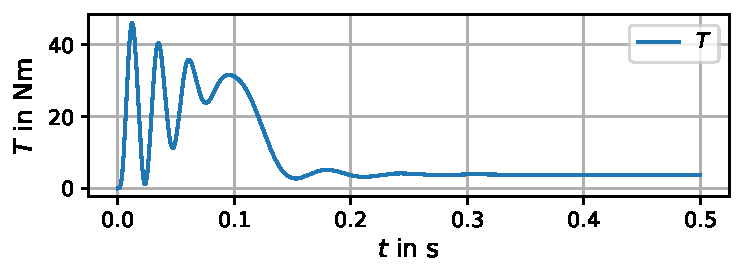
\includegraphics{ex05/torque_friction.pdf}
        \caption{Produced torque of an IM during the transient process and in the steady-state operation with a speed-dependent load.}
        \label{fig:torque_friction}
    \end{solutionfigure}
    \autoref{fig:torque_zoom_friction} shows a zoomed version of the produced torque to highlight the torque in the steady state.
    \begin{solutionfigure}[ht]
        \centering
        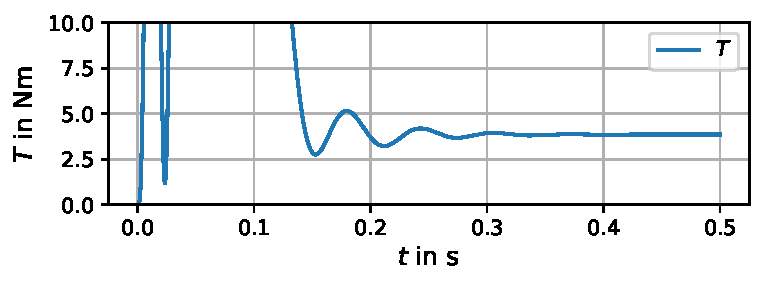
\includegraphics{ex05/torque_zoom_friction.pdf}
        \caption{Produced torque of an IM during the transient process and in the steady-state operation with a speed-dependent load.}
        \label{fig:torque_zoom_friction}
    \end{solutionfigure}

    In \autoref{fig:i_dq_friction} the currents in the dq coordinate system are visualized. Due to the load and, thus, the generated torque, the current $i_{\mathrm{q}}$ is no longer zero in the steady state. 
    \begin{solutionfigure}[ht]
        \centering
        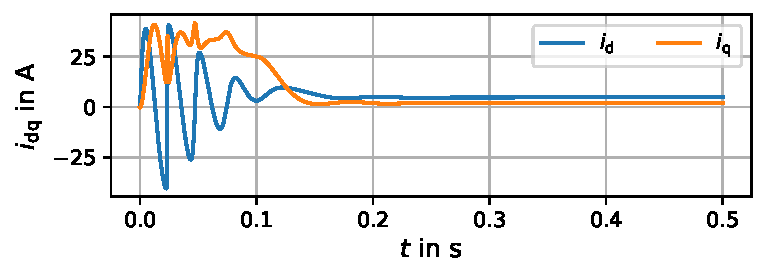
\includegraphics{ex05/i_dq_friction.pdf}
        \caption{Currents in dq coordinate system of an IM during the transient process and in the steady-state operation with a speed-dependent load.}
        \label{fig:i_dq_friction}
    \end{solutionfigure}

    \begin{solutionfigure}[ht]
        \centering
        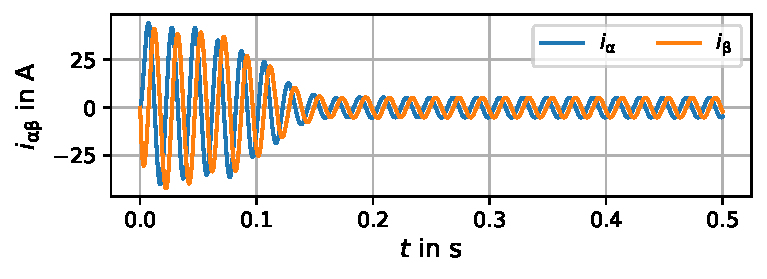
\includegraphics{ex05/i_alphaBeta_friction.pdf}
        \caption{Currents in $\upalpha \upbeta$ coordinate system of an IM during the transient process and in the steady-state operation with a speed-dependent load.}
        \label{fig:i_ab_friction}
    \end{solutionfigure}

    \begin{solutionfigure}[ht]
        \centering
        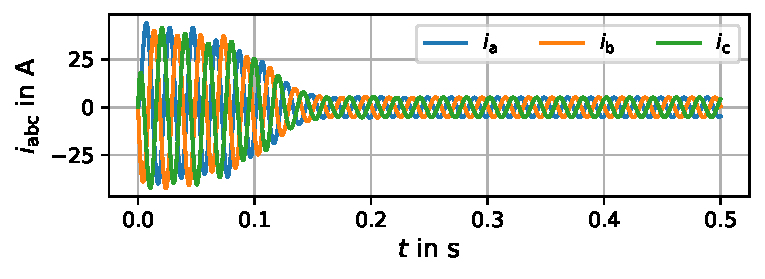
\includegraphics{ex05/i_abc_friction.pdf}
        \caption{Currents in abc coordinate system of an IM during the transient process and in the steady-state operation with a speed-dependent load.}
        \label{fig:i_abc_friction}
    \end{solutionfigure}

    \begin{solutionfigure}[ht]
        \centering
        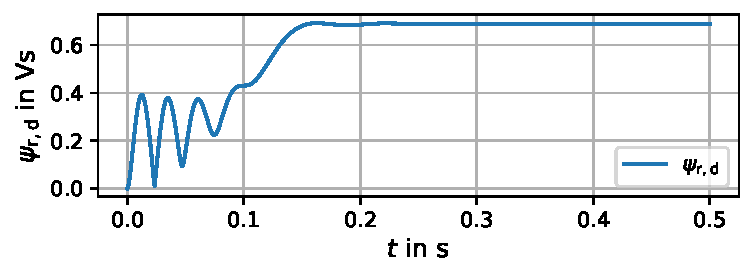
\includegraphics{ex05/psi_rd_friction.pdf}
        \caption{Rotor flux linkage in dq coordinate system of an IM during the transient process and in the steady-state operation with a speed-dependent load.}
        \label{fig:psi_rq_friction}
    \end{solutionfigure}

    \begin{solutionfigure}[ht]
        \centering
        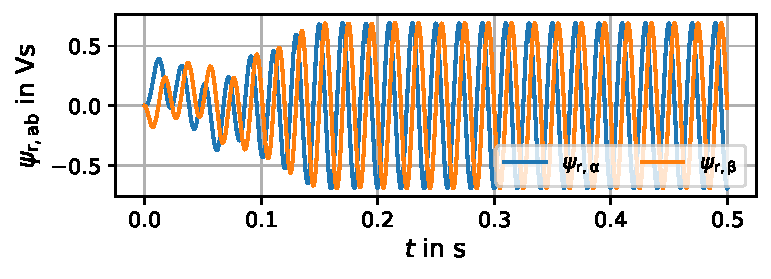
\includegraphics{ex05/psi_r_ab_friction.pdf}
        \caption{Rotor flux linkage in $\upalpha\upbeta$ coordinate system of an IM during the transient process and in the steady-state operation with a speed-dependent load.}
        \label{fig:psi_r_ab_friction}
    \end{solutionfigure}

    \begin{solutionfigure}[ht]
        \centering
        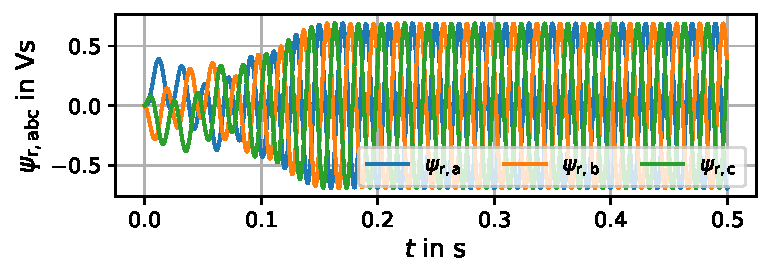
\includegraphics{ex05/psi_r_abc_friction.pdf}
        \caption{Rotor flux linkage in abc coordinate system of an IM during the transient process and in the steady-state operation with a speed-dependent load.}
        \label{fig:psi_r_abc_friction}
    \end{solutionfigure}



\end{solutionblock}


\FloatBarrier

%%%%%%%%%%%%%%%%%%%%%%%%%%%%%%%%%%%%%%%%%%%%%%%%%%%%%%%%%%%%%
%% Task 2 %%
%%%%%%%%%%%%%%%%%%%%%%%%%%%%%%%%%%%%%%%%%%%%%%%%%%%%%%%%%%%%%

\task{Steady-state operation of an induction machine}

An induction machine with the characteristics in Tab.~\ref{tab:characteristicsIM_task2} is given.
\begin{table}[htb]
    \caption{Characteristics of the given induction machine.}
    \centering
    \begin{tabular}{lll}\toprule
    Symbol  & Description       & Values \\
    \midrule
    $U_{\mathrm{n}}$    & Nominal voltage           & $\SI{380}{\volt}$ \\
    $I_{\mathrm{n}}$    & Nominal phase current     & $\SI{54}{\ampere}$ \\
    $f_{\mathrm{s,n}}$  & Nominal frequency         & $\SI{50}{\hertz}$ \\
    $P_{\mathrm{n}}$    & Nominal power             & $\SI{25}{\kilo\watt}$ \\
    $n_{\mathrm{n}}$    & Nominal speed             & $\SI{1465}{\per\minute}$ \\
    $\cos(\varphi)$     & Power factor              & 0.77 \\
    \midrule
    $R_{\mathrm{s}}$    & Stator resistance         & $\SI{0.48}{\Omega}$ \\
    $R_{\mathrm{r}}'$    & Rotor resistance          & $\SI{85}{\milli\Omega}$ \\
    $M$                 & Mutual inductance         & $\SI{100}{\milli\henry}$ \\
    $L_{\mathrm{\sigma,s}}$    & Stator leakage inductance  & $\SI{2}{\milli\henry}$ \\
    $L_{\mathrm{\sigma,r}}'$    & Rotor leakage inductance   & $\SI{2}{\milli\henry}$ \\
    \bottomrule
    \end{tabular}
    \label{tab:characteristicsIM_task2}
\end{table}


%%%%%%%%%%%%%%%%%%%%%%%%%%%%%%%%%%%%%%%%%%%%%%%%%%%%%%%%%%%%%
\subtask{Determine the amplitude of the complex AC voltage $\hat{U}$ and current phasor $\hat{I}$.}

\begin{solutionblock}
    The amplitude of the line-to-line voltage is given with
    \begin{equation}
    \hat{U} = \sqrt{2}\cdot \SI{380}{\volt}
    = \SI{537.4}{\volt},
    \end{equation}
    and, therefore, the amplitude of the phase-to-star-point voltage is defined as:
    \begin{equation}
    \hat{U}_{\mathrm{star}} = \frac{\SI{380}{\volt}}{\sqrt{3}}\cdot \sqrt{2} = \SI{310.9}{\volt}.
    \end{equation}

    Furthermore, the current amplitude is defined by:
    \begin{equation}
        \hat{I} = \sqrt{2} I = \sqrt{2} \cdot \SI{54}{\ampere} = \SI{76.4}{\ampere}.
    \end{equation}
\end{solutionblock}

%%%%%%%%%%%%%%%%%%%%%%%%%%%%%%%%%%%%%%%%%%%%%%%%%%%%%%%%%%%%%
\subtask{Determine the number of pole pairs $p$.}

\begin{solutionblock}
    The stator frequency is given with $f_{\mathrm{s}}$ = 50 Hz, which leads to the synchronous rotational speed of the electrical frequency as follows:
    \begin{equation}
        n_{\mathrm{syn,el}} = \SI{50}{\hertz} \cdot \SI{60}{\second\per\minute}
        = \SI{3000}{\per\minute}.
    \end{equation}
    
    The nominal speed is given with $n_{\mathrm{n}} = \SI{1465}{\per\minute}$, which is associated with a synchronous speed of $n_{\mathrm{syn,mech}} = \SI{1500}{\per\minute}$.
    
    Therefore, the number of pole pairs is defined with:
    \begin{equation}
        p = \frac{n_{\mathrm{syn,el}}}{n_{\mathrm{syn,mech}}}
        = \frac{\SI{3000}{\per\minute}}{\SI{1500}{\per\minute}}
        = 2.
    \end{equation}

\end{solutionblock}

%%%%%%%%%%%%%%%%%%%%%%%%%%%%%%%%%%%%%%%%%%%%%%%%%%%%%%%%%%%%%
\subtask{Calculate the rated slip $s_{\mathrm{n}}$. Which slip occurs at an ideal no-load operation (no firction)?}

\begin{solutionblock}
    The slip is calculated by:
    \begin{equation}
        s_{\mathrm{n}} = \frac{\omega_{\mathrm{slip,n}}}{\omega_{\mathrm{s}}}
        = \frac{\omega_{\mathrm{s}}-p \omega_{\mathrm{r}}}{\omega_{\mathrm{s}}}
        = \frac{\SI{2\pi\cdot \frac{3000}{60}}{\per\second}- 2 \cdot \SI{2\pi \cdot \frac{1465}{60}}{\per\second}}{\SI{2\pi \cdot \frac{3000}{60}}{\per\second}}
        = 0.023,
    \end{equation}
    where $\omega_{\mathrm{r}}$ is the rotor speed.
    At an ideal no-load operation (also no friction), the rotor has the same speed as the stator field and, therefore, $s$ = 0.
\end{solutionblock}

%%%%%%%%%%%%%%%%%%%%%%%%%%%%%%%%%%%%%%%%%%%%%%%%%%%%%%%%%%%%%
\subtask{Calculate the apparent, the reactive and the electrical power. In addition, determine the efficiency $\eta_{\mathrm{n}}$ for the rated operating point.}

\begin{solutionblock}
    The apparent power is calculated with
    \begin{equation}
        S = \sqrt{3} U I
        = \sqrt{3} \cdot \SI{380}{\volt} \cdot \SI{54}{\ampere}
        = \SI{35.541}{\kilo\volt\ampere},
    \end{equation}
    
    and, the electrical power is determined with the power factor in the task as follows:
    \begin{equation}
        P_{\mathrm{el,n}} = \sqrt{3} U I \cos(\varphi)
        = \sqrt{3} \cdot \SI{380}{\volt} \cdot \SI{54}{\ampere} \cdot 0.77
        = \SI{27.367}{\kilo\watt}.
    \end{equation}

    The angle of the phase shift is calculated by:
    \begin{equation}
        \varphi = \cos^{-1}(0.77) = \SI{39.6}{\degree}.
    \end{equation}

    Hence, the reactive power yields:
    \begin{equation}
        Q = \sqrt{3} U I \sin(\varphi)
        = \sqrt{3} \cdot \SI{380}{\volt} \cdot \SI{54}{\ampere} \cdot \sin(\SI{39.6}{\degree})
        = \SI{22.655}{\kilo\volt\ampere}.
    \end{equation}


    The efficiency results as:
    \begin{equation}
        \eta_{\mathrm{n}} = \frac{P_{\mathrm{mech,n}}}{P_{\mathrm{el,n}}} = \frac{\SI{25}{\kilo\watt}}{\SI{27.367}{\kilo\watt}}
        = 0.914.
    \end{equation}
\end{solutionblock}

%%%%%%%%%%%%%%%%%%%%%%%%%%%%%%%%%%%%%%%%%%%%%%%%%%%%%%%%%%%%%
\subtask{Determine the nominal torque generated by the induction machine.}

\begin{solutionblock}
    The torque is calculated as:
    \begin{equation}
        T_{\mathrm{n}} = \frac{P_{\mathrm{mech}}}{\omega_{\mathrm{mech}}}
        = \frac{\SI{25}{\kilo\watt}}{\SI{2\pi\cdot \frac{1465}{60}}{\per \second}}
        = \SI{163}{\newton \metre}.
    \end{equation}
\end{solutionblock}

%%%%%%%%%%%%%%%%%%%%%%%%%%%%%%%%%%%%%%%%%%%%%%%%%%%%%%%%%%%%%
\subtask{Calculate the starting $T_{\mathrm{0}}$ and the maximum torque $T_{\mathrm{max}}$. For the latter determine first the slip $s_{\mathrm{max}}$ at the operating point with the maximum torque.}

\begin{solutionblock}
    The slip at the maximum torque operating point is defined by
    \begin{equation}
        s_{\mathrm{max}} = \frac{R_{\mathrm{r}}'}{\sigma \left(L_{\mathrm{\sigma,r}}' + M\right) \omega_{\mathrm{s}}}
        = \frac{\SI{85}{\milli\Omega}}{0.038 \cdot (\SI{2}{\milli\henry}+\SI{100}{\milli\henry}) \cdot \SI{2\pi\cdot 50}{\per\second}}
        = 0.068,
    \end{equation}
    with the leakage coefficient:
    \begin{align}
        \begin{split}
            \sigma &= 1- \frac{M^2}{(M+L_{\mathrm{\sigma,s}})(M+L_{\mathrm{\sigma,r}}')}\\
            &= 1 - \frac{\left(\SI{100}{\milli\henry}\right)^2}{\left(\SI{102}{\milli\henry}\right)\cdot\left(\SI{102}{\milli\henry}\right)}\\
            &= 0.038.
        \end{split}
    \end{align}

    Hence, the maximum torque is calculated with:
    \begin{align}
        \begin{split}
            T_{\mathrm{max}} &= \frac{3}{2}p \frac{U_{\mathrm{s}}^2}{\omega_{\mathrm{s}}^2}\frac{M^2}{\sigma \left(L_{\mathrm{\sigma,s}}+M \right)^2\left(L_{\mathrm{\sigma,r}}'+M\right)} \\
            &= \frac{3}{2}\cdot2\cdot\frac{\frac{\SI{380}{\volt}}{\sqrt{3}}}{\left(\SI{2\pi\cdot 50}{\per\second}\right)^2} \cdot \frac{\SI{100}{\milli\henry}}{0.038\cdot\left(\SI{102}{\milli\henry}\right)^2 \cdot \left(\SI{102}{\milli\henry}\right)}\\
            &= \SI{355}{\newton\metre}.
        \end{split}
    \end{align}

    The starting torque is determined as follows:
    \begin{equation}
        T_{\mathrm{0}} = T_{\mathrm{max}} \frac{2 s_{\mathrm{max}}}{1 + s_{\mathrm{max}}^2}
        = \SI{355}{\newton\metre}\cdot \frac{2 \cdot 0.068}{1 + 0.068^2} = \SI{48.3}{\newton\metre}.
    \end{equation}
\end{solutionblock}


%%%%%%%%%%%%%%%%%%%%%%%%%%%%%%%%%%%%%%%%%%%%%%%%%%%%%%%%%%%%%
\subtask{Determine the stator currents $I_{\mathrm{s,dq}}$, and, in addition, the induced rotor currents $I_{\mathrm{r,dq}}$.}

\begin{solutionblock}
    Derived from the lecture notes, the stator currents are calculated as follows:
    \begin{align}
        \begin{split}
        I_{\mathrm{s,d}} &= \frac{U_{\mathrm{s}}}{\omega_{\mathrm{s}}} \frac{\sigma^2\omega_{\mathrm{slip}}^2 \left(L_{\mathrm{\sigma,s}}+M\right)\left(L_{\mathrm{\sigma,r}}'+M\right)^3 + \left(L_{\mathrm{\sigma,r}}'+M\right)\left(L_{\mathrm{\sigma,s}}+M\right)\left(R_{\mathrm{r}}'\right)^2 - M^2 \left(R_{\mathrm{r}}'\right)^2}{\sigma \left(L_{\mathrm{\sigma,s}}+M\right)^2 \left(L_{\mathrm{\sigma,r}}'+M\right)\omega_{\mathrm{slip}}\left(\sigma^2 \omega_{\mathrm{slip}}^2 \left(L_{\mathrm{\sigma,r}}'+M\right)^2 + \left(R_{\mathrm{r}}'\right)^2\right)}\\
        &= \SI{3.3}{\ampere},
        \end{split}
    \end{align}
    
    \begin{equation}
        I_{\mathrm{s,q}} = \frac{U_{\mathrm{s}}}{\omega_{\mathrm{s}}} \frac{M^2}{\sigma\left(L_{\mathrm{\sigma,s}}+M\right)^2 \left(L_{\mathrm{\sigma,r}}'+M\right)} \frac{1}{\frac{\omega_{\mathrm{slip}}}{\omega_{\mathrm{max}}} + \frac{\omega_{\mathrm{max}}}{\omega_{\mathrm{slip}}}}
        = \SI{51.8}{\ampere}.
    \end{equation}
    
    
    The rotor currents are calculated as follows:
    \begin{equation}
        I_{\mathrm{r,d}} = -U_{\mathrm{s}} \frac{M s}{\left(L_{\mathrm{\sigma,s}}+M\right) R_{\mathrm{r}}'}\frac{1}{\frac{\omega_{\mathrm{slip}}}{\omega_{\mathrm{max}}} + \frac{\omega_{\mathrm{max}}}{\omega_{\mathrm{slip}}}}
        = \SI{-18.06}{\ampere},
    \end{equation}

    \begin{equation}
        I_{\mathrm{r,q}} = -\frac{U_{\mathrm{s}}}{\omega_{\mathrm{s}}}\frac{M}{\sigma \left(L_{\mathrm{\sigma,s}}+M\right)\left(L_{\mathrm{\sigma,r}}'+M\right)}\frac{1}{\frac{\omega_{\mathrm{slip}}}{\omega_{\mathrm{max}}} + \frac{\omega_{\mathrm{max}}}{\omega_{\mathrm{slip}}}}
        = \SI{-52.9}{\ampere}.
    \end{equation}

    

\end{solutionblock}


%%%%%%%%%%%%%%%%%%%%%%%%%%%%%%%%%%%%%%%%%%%%%%%%%%%%%%%%%%%%%
\subtask{Calculate the losses in the stator winding and in the rotor.}

\begin{solutionblock}
    The stator current is determined by
    \begin{equation}
        I_{\mathrm{s,dq}} = \sqrt{I_{\mathrm{s,d}}^2 + I_{\mathrm{s,q}}^2}
        = \sqrt{\left(\SI{3.3}{\ampere}\right)^2 + \left(\SI{51.8}{\ampere}\right)^2}
        = \SI{51.9}{\ampere},
    \end{equation}
    which results to the stator winding losses as follows:
    \begin{equation}
        P_{\mathrm{l,stator}} = \frac{3}{2} I_{\mathrm{s,dq}}^2 R_{\mathrm{s}}
        = \frac{3}{2} \cdot \left(\SI{51.9}{\ampere} \right)^2 \cdot \SI{0.48}{\Omega}
        = \SI{1939.4}{\watt}.
    \end{equation}

    The rotor current is calculated in the same way. This leads to
    \begin{equation}
        I_{\mathrm{r,dq}} = \sqrt{I_{\mathrm{r,d}}^2 + I_{\mathrm{r,q}}^2}
        = \sqrt{\left(\SI{-18.1}{\ampere}\right)^2 + \left(\SI{-52.9}{\ampere}\right)^2}
        = \SI{55.9}{\ampere},
    \end{equation}
    and the ohmic rotor losses are calculated with:
    \begin{equation}
        P_{\mathrm{l,rotor}} = \frac{3}{2} I_{\mathrm{r,dq}}^2 R_{\mathrm{r}}'
        = \frac{3}{2} \cdot \left(\SI{55.9}{\ampere} \right)^2 \cdot \SI{85}{\milli\Omega}
        = \SI{398.4}{\watt}.
    \end{equation} 


\end{solutionblock}


%%%%%%%%%%%%%%%%%%%%%%%%%%%%%%%%%%%%%%%%%%%%%%%%%%%%%%%%%%%%%
\subtask{Draw the space vector diagram for the operation under rated conditions including the vectors $\underline{u}_{\mathrm{s}}$, $\underline{i}_{\mathrm{s}}$, $\underline{\psi}_{\mathrm{s}}$ and $\frac{\mathrm{d}}{\mathrm{d}t} \underline{\psi}_{\mathrm{s}}$. Assume that the current vector $\underline{i}_{\mathrm{s}}$ is oriented along the x-axis of the Cartesian coordinate system.}

\begin{solutionblock}
    The current is aligned with the x-axis of the Cartesian coordinate system. Therefore, the current is given with:
    \begin{equation}
        \underline{i}_{\mathrm{s}} = \sqrt{2} I e^{\mathrm{j}0^{\circ}}
        = \SI{76.37}{\ampere} \cdot e^{\mathrm{j}0^{\circ}}.
    \end{equation}

    The angle shift between the voltage and current is calculated by
    \begin{equation}
        \varphi_{\mathrm{ui}} = \SI{39.65}{\degree},
    \end{equation}

    therefore, the voltage is defined as follows:
    \begin{equation}
        \underline{u}_{\mathrm{s}} = \sqrt{2} U e^{\mathrm{j} \varphi_{\mathrm{ui}}}
        = \SI{310.27}{\volt} \cdot e^{\mathrm{j}39.65^{\circ}}
        = \SI{238.89}{\volt} + \mathrm{j} \SI{197.98}{\volt}.
    \end{equation}

    The stator resistance $R_{\mathrm{s}}$ is given in the task. Hence, the voltage equation is defined as:
    \begin{equation}
        \underline{u}_{\mathrm{s}} = R_{\mathrm{s}} \underline{i}_{\mathrm{s}} + \frac{\mathrm{d}}{\mathrm{d}t}\psi_{\mathrm{s}}.
    \end{equation}

    Rearranging leads to:
    \begin{align}
        \begin{split}
        \frac{\mathrm{d}}{\mathrm{d}t}\psi_{\mathrm{s}} &= \underline{u}_{\mathrm{s}} - R_{\mathrm{s}} \underline{i}_{\mathrm{s}} \\
        &= \SI{238.89}{\volt} + \mathrm{j} \SI{197.98}{\volt} - \SI{0.48}{\Omega} \cdot \SI{76.37}{\ampere} \\
        &= \SI{202.23}{\volt} + \mathrm{j} \SI{197.98}{\volt} \\
        &= \SI{283}{\volt} \cdot e^{\mathrm{j}44.4^{\circ}}.
        \end{split}
    \end{align}

    The stator flux vector is defined as
    \begin{equation}
        \underline{\psi}_{\mathrm{s}}(t) = \psi_{\mathrm{s}}(t) \cdot e^{\mathrm{j}\varphi_{\mathrm{s}}(t)},
    \end{equation}

    and the differentiation (under consideration of the product rule) results in:
    \begin{equation}
        \frac{\mathrm{d}}{\mathrm{d}t}\underline{\psi}_{\mathrm{s}}(t)
        = \frac{\mathrm{d}}{\mathrm{d}t} \psi_{\mathrm{s}}(t) \cdot e^{\mathrm{j}\varphi_{\mathrm{s}}(t)} + \mathrm{j} \omega_{\mathrm{\varphi_s}} \cdot \underline{\psi}_{\mathrm{s}}(t).
    \end{equation}

    Due to the steady state, the change of the flux amplitude $\left(\frac{\mathrm{d}}{\mathrm{d}t}\psi(t)\right)$ is zero. The flux vector rotates with the speed $\omega$, therefore, the flux vector is determined as follows:
    \begin{equation}
        \underline{\psi}_{\mathrm{s}}(t)
        = \frac{\SI{283}{\volt} \cdot e^{\mathrm{j}44.4^{\circ}}}{\SI{314.16}{\per\second}\cdot e^{\mathrm{j}90^{\circ}}}
        = \SI{0.90}{\volt\second} \cdot e^{-\mathrm{j}\SI{45.6}{\degree}}.
    \end{equation}


    \begin{solutionfigure}
        \centering
        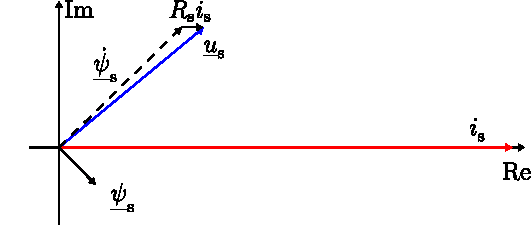
\includegraphics{ex05/vectorDiagram_IM.pdf}
        \caption{Resulting vector diagram of the induction machine in steady state. The scala for the voltage is 1 cm $\widehat{=}~\SI{100}{\volt} $, for the flux linkage 1 cm $\widehat{=}~\SI{1}{\volt\second}$ and for the current 1 cm $\widehat{=}~\SI{10}{\ampere}$.}
        \label{fig:vectorDiagram_IM}
    \end{solutionfigure}


\end{solutionblock}
    %%%%%%%%%%%%%%%%%%%%%%%%%%%%%%%%%%%%%%%%%%%%%%%%%%%%%%%%%%%%%
%% Begin exercise %%
%%%%%%%%%%%%%%%%%%%%%%%%%%%%%%%%%%%%%%%%%%%%%%%%%%%%%%%%%%%%%
\ex{Synchronous machines}


\normalsize{\textbf{Acknowledgement}: Parts of the following exercise are adapted from ``Elektrische Antriebstechnik'' by J. Böcker, Paderborn University, 2020
}\\



%%%%%%%%%%%%%%%%%%%%%%%%%%%%%%%%%%%%%%%%%%%%%%%%%%%%%%%%%%%%%
%% Task 1 %%
%%%%%%%%%%%%%%%%%%%%%%%%%%%%%%%%%%%%%%%%%%%%%%%%%%%%%%%%%%%%%

\task{Transient simulation of a salient pole synchronous machine}
Given is a salient pole synchronous machine with the parameters in Tab.~\ref{tab:para_salientSynchonousMachine}.

\begin{table}[htb]
    \caption{Parameters of the salient synchronous machine.}
    \centering
    \begin{tabular}{lll}\toprule
    Symbol  & Description       & Value \\
    \midrule
    $R_{\mathrm{s}}$    & Stator resistance         & $\SI{0.0196}{\Omega}$ \\
    $R_{\mathrm{f}}$    & Field winding resistance  & $\SI{54.7}{\Omega}$ \\
    $L_{\mathrm{s,d}}$    & Stator inductance d-axis  & $\SI{2.7}{\milli\henry}$ \\
    $L_{\mathrm{s,q}}$    & Stator inductance q-axis  & $\SI{1.3}{\milli\henry}$ \\
    $L_{\mathrm{f}}$    & Self field inductance     & $\SI{20.3}{\milli\henry}$ \\
    $M_{\mathrm{fs}}$   & Mutual inductance         & $\SI{92.8}{\milli\henry}$ \\
    $I_{\mathrm{n}}$    & Nominal stator current    & $\SI{450}{\ampere}$ \\
    $I_{\mathrm{f,n}}$  & Nominal field current     & $\SI{7.854}{\ampere}$ \\
    \bottomrule
    \end{tabular}
    \label{tab:para_salientSynchonousMachine}
\end{table}






%%%%%%%%%%%%%%%%%%%%%%%%%%%%%%%%%%%%%%%%%%%%%%%%%%%%%%%%%%%%%
\subtask{Calculate the transient response for $i_{\mathrm{dq}}$ and $i_{\mathrm{f}}$ if a short circuit occurs at the running machine. Assume $i_{\mathrm{d0}} = i_{\mathrm{q0}}$ = 0, $i_{\mathrm{f0}} = i_{\mathrm{f,n}}$ for $t=0$ and a fixed rotational speed $\omega_{\mathrm{r,el}}$. Assume further that the ohmic stator resistance can be neglected for the short-term transient response.}


\begin{solutionblock}
    
    The machine model is defined as
    \begin{align}
        \begin{split}
        \frac{\mathrm{d}}{\mathrm{d}t}
        &
        \begin{bmatrix}
            i_{\mathrm{s,d}}(t) \\
            i_{\mathrm{s,q}}(t) \\
            i_{\mathrm{f}}(t)
        \end{bmatrix}
        =
        \begin{bmatrix}
            -L_{\mathrm{f}}/\gamma  & 0 & M_{\mathrm{fs}}/\gamma \\
            0                       & 1/L_{\mathrm{s,q}}  & 0 \\
            M_{\mathrm{fs}}/\gamma  & 0 & -L_{\mathrm{s,d}}/\gamma 
        \end{bmatrix} \\
        &
        \begin{pmatrix}
            \begin{bmatrix}
                u_{\mathrm{s,d}}(t) \\
                u_{\mathrm{s,q}}(t) \\
                u_{\mathrm{f}}(t)
            \end{bmatrix}
            -
            \begin{bmatrix}
                R_{\mathrm{s}}  & 0 & 0 \\
                0 & R_{\mathrm{s}} & 0 \\
                0 & 0 & R_{\mathrm{f}}
            \end{bmatrix}
            \begin{bmatrix}
                i_{\mathrm{s,d}}(t) \\
                i_{\mathrm{s,q}}(t) \\
                i_{\mathrm{f}}(t)
            \end{bmatrix}
            -
            \begin{bmatrix}
                0 & -\omega_{\mathrm{r,el}}(t) & 0 \\
                \omega_{\mathrm{r,el}}(t) & 0 & 0 \\
                0 & 0 & 0
            \end{bmatrix}
            \begin{bmatrix}
                \psi_{\mathrm{s,d}}(t) \\
                \psi_{\mathrm{s,q}}(t) \\
                \psi_{\mathrm{f}}(t)
            \end{bmatrix}
        \end{pmatrix},
        \label{eq:model_sm}
    \end{split}
    \end{align}

    with the parameter 
    \begin{equation}
        \gamma = M_{\mathrm{fs}}^2-L_{\mathrm{s,d}}L_{\mathrm{f}},
    \end{equation}
    and the flux linkages
    \begin{equation}
        \begin{bmatrix}
            \psi_{\mathrm{s,d}}(t) \\
            \psi_{\mathrm{s,q}}(t) \\
            \psi_{\mathrm{f}}(t)
        \end{bmatrix}
        =
        \begin{bmatrix}
            L_{\mathrm{s,d}}  & 0     & M_{\mathrm{fs}} \\
            0       & L_{\mathrm{s,q}}    & 0 \\
            M_{\mathrm{fs}}     & 0     & L_{\mathrm{f}}
        \end{bmatrix}
        \begin{bmatrix}
            i_{\mathrm{s,d}}(t) \\
            i_{\mathrm{s,q}}(t) \\
            i_{\mathrm{f}}(t)
        \end{bmatrix}.
    \end{equation}



    With the assumption of a constant speed ($\omega_{\mathrm{r,el}}(t) =\omega_{\mathrm{r,el}}$), the general machine model from \eqref{eq:model_sm} is rewritten as follows:
    \begin{align}
        \begin{split}
        \frac{\mathrm{d}}{\mathrm{d}t}
        \begin{bmatrix}
            i_{\mathrm{s,d}}(t) \\
            i_{\mathrm{s,q}}(t) \\
            i_{\mathrm{f}}(t)
        \end{bmatrix}
        = &
        \begin{bmatrix}
            L_{\mathrm{f}}R_{\mathrm{s}}/\gamma     & -L_{\mathrm{f}}L_{\mathrm{s,q}}\omega_{\mathrm{r,el}}/\gamma & -M_{\mathrm{fs}}R_{\mathrm{f}}/\gamma \\
            -L_{\mathrm{s,d}}\omega_{\mathrm{r,el}}/L_{\mathrm{s,q}} & -R_{\mathrm{s}}/L_{\mathrm{s,q}} & -M_{\mathrm{fs}}\omega_{\mathrm{r,el}}/L_{\mathrm{s,q}} \\
            -M_{\mathrm{fs}}R_{\mathrm{s}}/\gamma & M_{\mathrm{fs}}L_{\mathrm{s,q}}\omega_{\mathrm{r,el}} / \gamma & L_{\mathrm{s,d}}R_{\mathrm{f}}/\gamma 
        \end{bmatrix}
        \begin{bmatrix}
            i_{\mathrm{s,d}}(t) \\
            i_{\mathrm{s,q}}(t) \\
            i_{\mathrm{f}}(t)
        \end{bmatrix}
        \\
        + &
        \begin{bmatrix}
            -L_{\mathrm{f}}/\gamma & 0 & M_{\mathrm{fs}}/\gamma \\
            0 & 1/L_{\mathrm{s,q}} & 0 \\
            M_{\mathrm{fs}}/\gamma & 0 & -L_{\mathrm{s,d}}/\gamma
        \end{bmatrix}
        \begin{bmatrix}
            u_{\mathrm{s,d}}(t) \\
            u_{\mathrm{s,q}}(t) \\
            u_{\mathrm{f}}(t)
        \end{bmatrix}.
    \end{split}
    \end{align}
    
    The exact system response is calculated with:
    \begin{equation}
        \bm{x}(t) = \bm{\Phi}(t,t_{\mathrm{0}})\bm{x}_{\mathrm{0}} + \int_{t_{\mathrm{0}}}^{t}\bm{\Phi}(t,\tau)\bm{B}\bm{u}(\tau) \mathrm{d}\tau,
    \end{equation}
    with
    \begin{equation}
        \bm{x}_{\mathrm{0}} = \bm{x}(t_{\mathrm{0}}),
    \end{equation}
    and,
    \begin{equation}
        \bm{\Phi}(t,t_{\mathrm{0}}) = e^{\bm{A}(t-t_{\mathrm{0}})}.
    \end{equation}
    

   To calculate the transient system response without damping, the resistances are assumed to be zero. Hence, the equation is simplifies to:
    \begin{align}
        \begin{split}
        \underbrace{
        \frac{\mathrm{d}}{\mathrm{d}t}
        \begin{bmatrix}
            i_{\mathrm{s,d}}(t) \\
            i_{\mathrm{s,q}}(t) \\
            i_{\mathrm{f}}(t)
        \end{bmatrix}}_{\frac{\mathrm{d}}{\mathrm{d}t}\bm{x}(t)}
        =
        &
        \underbrace{
        \begin{bmatrix}
            0   & -L_{\mathrm{f}}L_{\mathrm{s,q}}\omega_{\mathrm{r,el}}/ \gamma   & 0 \\
            -L_{\mathrm{s,d}}\omega_{\mathrm{r,el}}/ L_{\mathrm{s,q}} & 0 & -M_{\mathrm{fs}}\omega_{\mathrm{r,el}} / L_{\mathrm{s,q}} \\
            0 & M_{\mathrm{fs}}L_{\mathrm{s,q}}\omega_{\mathrm{r,el}} / \gamma & 0
        \end{bmatrix}}_{\bm{A}}
        \underbrace{
        \begin{bmatrix}
            i_{\mathrm{s,d}}(t) \\
            i_{\mathrm{s,q}}(t) \\
            i_{\mathrm{f}}(t)
        \end{bmatrix}}_{\bm{x}(t)}
        \\
        + &
        \underbrace{
        \begin{bmatrix}
            -L_{\mathrm{f}}/\gamma & 0 & M_{\mathrm{fs}}/\gamma \\
            0 & 1/L_{\mathrm{s,q}} & 0 \\
            M_{\mathrm{fs}}/\gamma & 0 & -L_{\mathrm{s,d}}/\gamma
        \end{bmatrix}}_{\bm{B}}
        \underbrace{
        \begin{bmatrix}
            u_{\mathrm{s,d}}(t) \\
            u_{\mathrm{s,q}}(t) \\
            u_{\mathrm{f}}(t)
        \end{bmatrix}}_{\bm{u}(t)}.
    \end{split}
    \end{align}

    The eigenvalues of $\bm{A}$ are determined by:
    \begin{align}
        \begin{split}
        &\mathrm{det}\left(
            \begin{bmatrix}
                \lambda & L_{\mathrm{f}}L_{\mathrm{s,q}}\omega_{\mathrm{r,el}} /\gamma & 0 \\
                L_{\mathrm{s,d}}\omega_{\mathrm{r,el}} / L_{\mathrm{s,q}} & \lambda & M_{\mathrm{fs}}\omega_{\mathrm{r,el}}/L_{\mathrm{s,q}} \\
                0 & -M_{\mathrm{fs}}L_{\mathrm{s,q}}\omega_{\mathrm{r,el}} / \gamma & \lambda
            \end{bmatrix}
        \right)
        = 0 \\
        &= \lambda^3 + \frac{M_{\mathrm{fs}}\omega_{\mathrm{r,el}}^2}{\gamma}\lambda - \frac{L_{\mathrm{f}}L_{\mathrm{s,d}}\omega_{\mathrm{r,el}}^2}{\lambda}\gamma \\
        &= \lambda\left(\lambda^2+\frac{\omega_{\mathrm{r,el}}^2}{\gamma}M_{\mathrm{fs}}^2-L_{\mathrm{f}}L_{\mathrm{s,d}}\right).
    \end{split}
    \end{align}

    This results in the following eigenvalues, $\lambda_{\mathrm{1,2,3}} = \left\{+\mathrm{j}\omega_{\mathrm{r,el}}, -\mathrm{j}\omega_{\mathrm{r,el}}, 0 \right\}$.


    The following transition matrix results from the calculated eigenvalues
    \begin{equation}
        \bm{\Phi}(t,t_{\mathrm{0}}) = e^{\bm{A}(t-t_{\mathrm{0}})} = \bm{P} \mathrm{diag}\left(e^{\lambda_{\mathrm{1}}(t-t_{\mathrm{0}})}, ..., e^{\lambda_n(t-t_{\mathrm{0}})}\right)\bm{P}^{-1},
    \end{equation}
    with $\bm{P}$ and $\bm{P}^{-1}$ holding the left and right eigenvectors of $\bm{A}$ leading to
    \begin{align}
        \begin{split}
            \bm{\Phi}(t,t_{\mathrm{0}}) =
        &
        \begin{bmatrix}
            \frac{-M_{\mathrm{fs}}}{L_{\mathrm{s,d}}}     & \frac{-L_{\mathrm{f}}}{M_{\mathrm{fs}}} & \frac{-L_{\mathrm{f}}}{M_{\mathrm{fs}}} \\
            0 & \frac{-\mathrm{j}\gamma }{(L_{\mathrm{s,d}}M_{\mathrm{fs}})} & \frac{\mathrm{j}\gamma }{(L_{\mathrm{s,q}}M_{\mathrm{fs}})} \\
            1 & 1 & 1
        \end{bmatrix}
        \begin{bmatrix}
            e^{0(t-t_{\mathrm{0}})} & 0 & 0 \\
            0 & e^{-\mathrm{j}\omega_{\mathrm{r,el}}(t-t_{\mathrm{0}})} & 0 \\
            0 & 0 & e^{\mathrm{j}\omega_{\mathrm{r,el}}(t-t_{\mathrm{0}})}
        \end{bmatrix}
        \\
        &
        \begin{bmatrix}
            \frac{-M_{\mathrm{fs}}L_{\mathrm{s,d}}}{\gamma} & 0 & \frac{-L_{\mathrm{f}}L_{\mathrm{s,d}}}{\gamma} \\
            \frac{M_{\mathrm{fs}}L_{\mathrm{s,d}}}{2\gamma} & \frac{\mathrm{j}L_{\mathrm{s,q}}M_{\mathrm{fs}}}{2\gamma} & \frac{M_{\mathrm{fs}}^2}{2\gamma} \\
            \frac{M_{\mathrm{fs}}L_{\mathrm{s,d}}}{2\gamma} & \frac{-\mathrm{j}L_{\mathrm{s,q}}M_{\mathrm{fs}}}{2\gamma} & \frac{M_{\mathrm{fs}}^2}{2\gamma}
        \end{bmatrix}
        \\ = &
        \begin{bmatrix}
            \frac{M_{\mathrm{fs}}^2 - L_{\mathrm{s,d}}L_{\mathrm{f}}\cos((t-t_{\mathrm{0}})\omega_{\mathrm{r,el}}}{\gamma} & \frac{-L_{\mathrm{s,q}}L_{\mathrm{f}}\sin((t-t_{\mathrm{0}})\omega_{\mathrm{r,el}})}{\gamma} & \frac{-L_{\mathrm{f}}M_{\mathrm{fs}}(\cos((t-t_{\mathrm{0}})\omega_{\mathrm{r,el}})-1)}{\gamma} \\
            \frac{-L_{\mathrm{s,d}}\sin((t-t_{\mathrm{0}})\omega_{\mathrm{r,el}})}{L_{\mathrm{s,q}}} & \cos((t-t_{\mathrm{0}})\omega_{\mathrm{r,el}}) & \frac{-M_{\mathrm{fs}}\sin((t-t_{\mathrm{0}})\omega_{\mathrm{r,el}})}{L_{\mathrm{s,q}}} \\
            \frac{L_{\mathrm{s,d}}M_{\mathrm{fs}}(\cos((t-t_{\mathrm{0}})\omega_{\mathrm{r,el}})-1)}{\gamma} & \frac{L_{\mathrm{s,q}}M_{\mathrm{fs}}\cos((t-t_{\mathrm{0}})\omega_{\mathrm{r,el}})}{\gamma} & \frac{M_{\mathrm{fs}}^2\cos((t-t_{\mathrm{0}})\omega_{\mathrm{r,el}})-L_{\mathrm{s,d}}L_{\mathrm{f}}}{\gamma}
        \end{bmatrix}.
        \end{split}
    \end{align}


    In the task, the short circuit case of the machine is given, therefore, the input voltage is zero, which leads to
    \begin{equation}
        \begin{bmatrix}
            i_{\mathrm{s,d}}(t) \\
            i_{\mathrm{s,q}}(t) \\
            i_{\mathrm{f}}(t) \\
        \end{bmatrix}
        = \bm{x}(t) = \bm{\Phi}(t,t_{\mathrm{0}})\bm{x}_{\mathrm{0}} + 
        \underbrace{
        \int_{t_{\mathrm{0}}}^{t}\bm{\Phi}(t,\tau)\bm{B}\bm{u}(\tau) \mathrm{d}\tau}_{0},
    \end{equation}
    and the given assumption for the initial states:
    \begin{equation}
        x_{\mathrm{0}} =
        \begin{bmatrix}
            0 \\
            0 \\
            i_{\mathrm{f,0}}
        \end{bmatrix}.
    \end{equation}

    This results into the analytical solution:
    \begin{align}
        \begin{split}
        \begin{bmatrix}
            i_{\mathrm{s,d}}(t) \\
            i_{\mathrm{s,q}}(t) \\
            i_{\mathrm{f}}(t) \\
        \end{bmatrix}
        &= 
        \begin{bmatrix}
            \frac{M_{\mathrm{fs}}^2 - L_{\mathrm{s,d}}L_{\mathrm{f}}\cos(t\omega_{\mathrm{r,el}})}{\gamma} & \frac{-L_{\mathrm{s,q}}L_{\mathrm{f}}\sin(t\omega_{\mathrm{r,el}})}{\gamma} & \frac{-L_{\mathrm{f}}M_{\mathrm{fs}}(\cos(t\omega_{\mathrm{r,el}})-1)}{\gamma} \\
            \frac{-L_{\mathrm{s,d}}\sin(t\omega_{\mathrm{r,el}})}{L_{\mathrm{s,q}}} & \cos(t\omega_{\mathrm{r,el}}) & \frac{-M_{\mathrm{fs}}\sin(t\omega_{\mathrm{r,el}})}{L_{\mathrm{s,q}}} \\
            \frac{L_{\mathrm{s,d}}M_{\mathrm{fs}}(\cos(t\omega_{\mathrm{r,el}})-1)}{\gamma} & \frac{L_{\mathrm{s,q}}M_{\mathrm{fs}}\cos(t\omega_{\mathrm{r,el}})}{\gamma} & \frac{M_{\mathrm{fs}}^2\cos(t\omega_{\mathrm{r,el}})-L_{\mathrm{s,d}}L_{\mathrm{f}}}{\gamma}
        \end{bmatrix}
        \begin{bmatrix}
            0 \\
            0 \\
            i_{\mathrm{f0}}
        \end{bmatrix} \\
        &=
        \begin{bmatrix}
            \frac{-L_{\mathrm{f}}M_{\mathrm{fs}}(\cos(t\omega_{\mathrm{r,el}})-1)}{\gamma} \\
            \frac{-M_{\mathrm{fs}}\sin(t\omega_{\mathrm{r,el}})}{L_{\mathrm{s,q}}} \\
            \frac{M_{\mathrm{fs}}^2 \cos(t\omega_{\mathrm{r,el}}) -L_{\mathrm{s,d}}L_{\mathrm{f}}}{\gamma}
        \end{bmatrix}
        i_{\mathrm{f0}}.
    \end{split}
    \end{align}

\end{solutionblock}






%%%%%%%%%%%%%%%%%%%%%%%%%%%%%%%%%%%%%%%%%%%%%%%%%%%%%%%%%%%%%
\subtask{Determine the maximum current $|i_{\mathrm{s,dq}}|$ for this scenario.}

\begin{solutionblock}
    The quadratic current amplitude is given with:
    \begin{equation}
        i_{\mathrm{s,dq}}^2(t) = i_{\mathrm{s,d}}^2(t) + i_{\mathrm{s,q}}^2(t)
        = i_{\mathrm{f0}}^2 M_{\mathrm{fs}}^2 \left(\frac{L_{\mathrm{f}}^2}{\gamma^2}(\cos(t\omega_{\mathrm{r,el}})-1)^2 + \frac{1}{L_{\mathrm{s,q}}^2}\sin(t\omega_{\mathrm{r,el}})^2\right).
    \end{equation}

    To determine the maximum current, the first derivative is calculated and set to zero, which is given as:
    \begin{equation}
        \frac{\mathrm{d}}{\mathrm{d}t} i_{\mathrm{s,dq}}^2(t)
        = i_{\mathrm{f0}}M_{\mathrm{fs}}^2 \omega_{\mathrm{r,el}} 
        \underbrace{
        \left(-2\frac{L_{\mathrm{f}}^2}{\gamma^2}\sin(t\omega_{\mathrm{r,el}}) (\cos(t\omega_{\mathrm{r,el}})-1) + \frac{1}{L_{\mathrm{s,q}}^2} \cos(t\omega_{\mathrm{r,el}}) \sin(t\omega_{\mathrm{r,el}}) \right)
        }_{t_{\mathrm{dq}}^{*}}
        = 0.
    \end{equation}

    In the next step, the value of $t_{\mathrm{dq}}^*$ is determined, so that the expression inside the brackets is zero.
    Hence, the maximum $t_{\mathrm{dq}}^*$ is calculated with:
    \begin{equation}
        t_{\mathrm{dq}}^{*} = \mathrm{arg}\max\limits_{t} i_{\mathrm{s,dq}}(t)
        = \frac{1}{\omega_{\mathrm{r,el}}} \mathrm{acos} \left(\frac{L_{\mathrm{f}}^2 L_{\mathrm{s,q}}^2}{L_{\mathrm{f}}^2 L_{\mathrm{s,q}}^2 - \gamma^2}\right) + \frac{2\pi}{\omega_{\mathrm{r,el}}}i,
    \end{equation}
    for $i$ = 0,1,2,... . This leads to the maximum current amplitude of:
    \begin{equation}
        i_{\mathrm{s,dq}} = \frac{i_{\mathrm{f0}} M_{\mathrm{fs}} |\gamma| }{L_{\mathrm{s,q}} \sqrt{\gamma^2 - L_{\mathrm{f}}^2 L_{\mathrm{s,q}}^2}}
        = \SI{683}{\ampere}.
    \end{equation}
\end{solutionblock}


%%%%%%%%%%%%%%%%%%%%%%%%%%%%%%%%%%%%%%%%%%%%%%%%%%%%%%%%%%%%%
\subtask{Write a Jupyter notebook to simulate the short transient response of the machine under the same initial conditions using an ODE solver. Compare the result including the impact of the stator resistance with the simplified analytical solution from the previous task. The simulation configuration is given in Tab.~\ref{tab:config_simulation}.}

\begin{table}[htb]
    \caption{Configuration of the simulation.}
    \centering
    \begin{tabular}{lll}\toprule
    Symbol  & Description       & Value \\
    \midrule
    $T_{\mathrm{sim}}$  & Simulation time           & $\SI{0.05}{\second}$ \\
    $\varepsilon_{\mathrm{m,0}}$    & Start angle of the rotor  & $\SI{0}{\degree}$ \\
    $\omega_{\mathrm{m,0}}$    & Start speed of the rotor  & $\SI{628.3}{\per\second}$ \\
    \bottomrule
    \end{tabular}
    \label{tab:config_simulation}
\end{table}


\begin{solutionblock}
    Beside the stator current ODEs, the mechanical system of the machine must be considered, therefore, the generated torque is calculated with
    \begin{equation}
        T(t) = \frac{3}{2}p\left(M_{\mathrm{fs}}i_{\mathrm{f}}(t) + \left(L_{\mathrm{s,d}}-L_{\mathrm{s,q}}\right)i_{\mathrm{s,q}}(t)i_{\mathrm{s,d}}(t)\right),
    \end{equation}
    and the mechanical equation is defined as follows:
    \begin{equation}
        \frac{\mathrm{d}}{\mathrm{d}t} \omega(t) = \frac{p}{J} \left(T(t)-T_{\mathrm{l}}(t)\right).
    \end{equation}

    The relationship between the angle and the rotational speed is given by:
    \begin{equation}
        \frac{\mathrm{d}}{\mathrm{d}t} \varepsilon(t) = \omega(t).
    \end{equation}

    In \autoref{fig:i_dq_omega_const_analytical_ode} a comparison between the analytical and the numerical solution of is shown. The currents are initialized with the same values at $t=0$. The trajectories of the analytical and the numerical current values are identical, except that a damping behavior is visible in the numerical solution. This results from the consideration of the winding resistances in the numerical solution, in comparison to the simplified analytical one.
    \begin{solutionfigure}[ht]
        \centering
        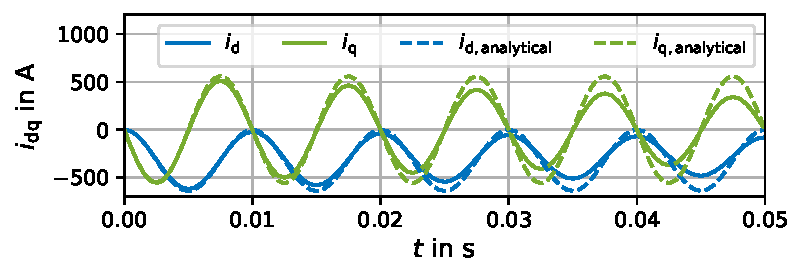
\includegraphics{ex06/i_dq_omega_const_analytical_ode.pdf}
        \caption{Transient process of $i_{\mathrm{dq}}$ of a salient synchronous machine with a stator and field winding short circuit.}
        \label{fig:i_dq_omega_const_analytical_ode}
    \end{solutionfigure}

    The trajectories of the field current $i_{\mathrm{f}}$ are visualized in \autoref{fig:i_f_omega_const_analytical_ode}. The behavior of this two trajectories are identical, except to the damping in the numerical solution, due to the considered winding resistance.
    \begin{solutionfigure}[ht]
        \centering
        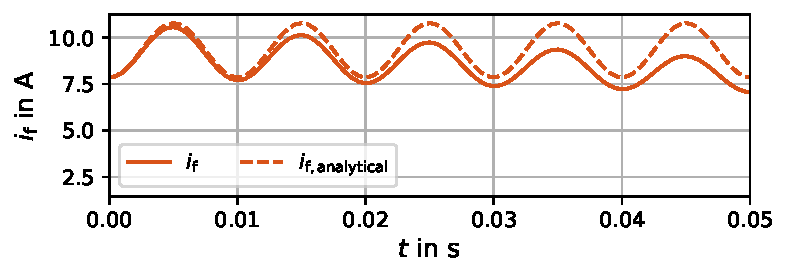
\includegraphics{ex06/i_f_omega_const_analytical_ode.pdf}
        \caption{Transient process of the field current $i_{\mathrm{f}}$ of a salient synchronous machine with a stator and field winding short circuit.}
        \label{fig:i_f_omega_const_analytical_ode}
    \end{solutionfigure}

\end{solutionblock}

\FloatBarrier

%%%%%%%%%%%%%%%%%%%%%%%%%%%%%%%%%%%%%%%%%%%%%%%%%%%%%%%%%%%%%
\subtask{Add a load with the following characteristic $T_{\mathrm{l}}(t) = 0.0001\cdot \omega_{\mathrm{r}}^{2}(t)$ to the existing simulation. Repeat the simulation with the same initial conditions as in the task before. Extend the simulation time to $T_{\mathrm{sim}} = \SI{0.5}{\second}$ and plot the currents $i_{\mathrm{d}}(t)$, $i_{\mathrm{f}}(t)$, the angular frequency of the rotor $\omega_{\mathrm{r,el}}(t)$ and the torque $T(t)$.}

\begin{solutionblock}
    The resulting currents for the new operating point are shown in \autoref{fig:i_dq_ode}.
    \begin{solutionfigure}[ht]
        \centering
        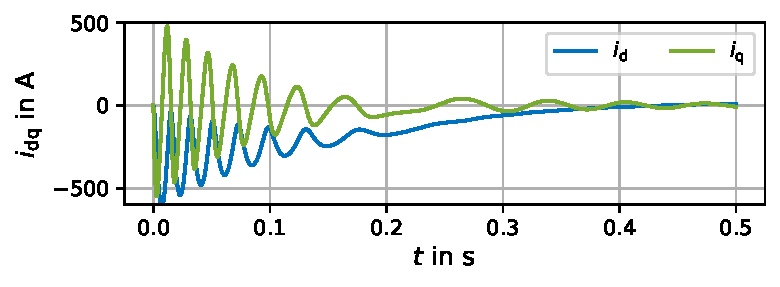
\includegraphics{ex06/i_dq_ode.pdf}
        \caption{Transient process of $i_{\mathrm{dq}}$ of a salient synchronous machine with a stator and field winding short circuit and a load resistance.}
        \label{fig:i_dq_ode}
    \end{solutionfigure}

    The filed winding current is visualized in \autoref{fig:i_f_ode}.
    \begin{solutionfigure}[ht]
        \centering
        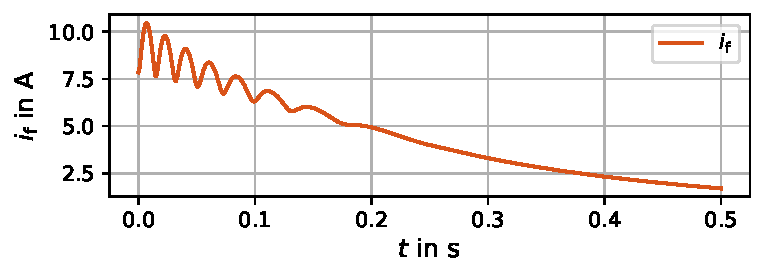
\includegraphics{ex06/i_f_ode.pdf}
        \caption{Transient process of $i_{\mathrm{f}}$ of a salient synchronous machine with a stator and field winding short circuit and a load resistance.}
        \label{fig:i_f_ode}
    \end{solutionfigure}

    Fig~\ref{fig:omega_r_el_ode} shows the angular frequency of the rotor. Due to the winding resistance and the additional load, the currents are reduced over time, until the machine comes to a standstill.
    \begin{solutionfigure}[ht]
        \centering
        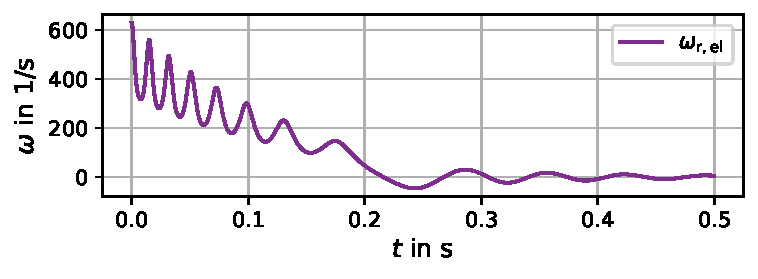
\includegraphics{ex06/omega_r_el_ode.pdf}
        \caption{Transient process of a salient synchronous machine with a stator and field winding short circuit and a load resistance.}
        \label{fig:omega_r_el_ode}
    \end{solutionfigure}

    The generated torque during the transient process is shown in \autoref{fig:T_ode}.
    \begin{solutionfigure}[ht]
        \centering
        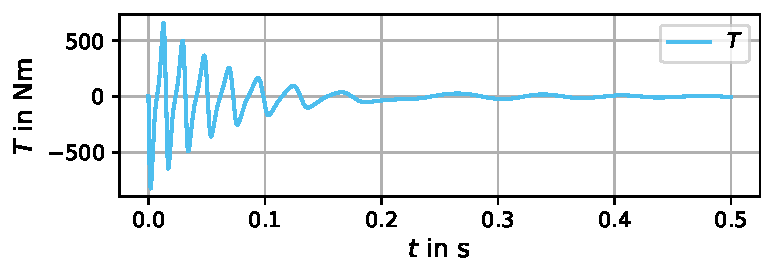
\includegraphics{ex06/T_ode.pdf}
        \caption{Generated torque of a salient synchronous machine with a stator and field winding short circuit and a load resistance.}
        \label{fig:T_ode}
    \end{solutionfigure}


\end{solutionblock}

\FloatBarrier

%%%%%%%%%%%%%%%%%%%%%%%%%%%%%%%%%%%%%%%%%%%%%%%%%%%%%%%%%%%%%
\subtask{Now consider an additional damper winding with the parameters from Tab.~\ref{tab:para_damperWinding} in the simulation. Compare the resulting current signalforms, the speed and the generated torque to the previous tasks with the identical simulation configuration as in the previous tasks. Consider the damper winding to not carry any current for $t$ = 0.}

\begin{table}[htb]
    \caption{Parameters of the damper winding.}
    \centering
    \begin{tabular}{lll}\toprule
    Symbol  & Description       & Value \\
    \midrule
    $M_{\mathrm{dD}}$   & Mutual ind. rotor d-axis  & $\SI{2}{\milli\henry}$ \\
    $M_{\mathrm{qQ}}$   & Mutual ind. rotor q-axis  & $\SI{1}{\milli\henry}$ \\
    $M_{\mathrm{fr}}$   & Mutual ind. field-rotor   & $\SI{50}{\milli\henry}$ \\
    $L_{\mathrm{D}}$    & Self ind. rotor d-axis    & $\SI{3}{\milli\henry}$ \\
    $L_{\mathrm{Q}}$    & Self ind. rotor q-axis    & $\SI{2}{\milli\henry}$ \\
    $R_{\mathrm{rD}}$   & Rotor winding res. d-axis & $\SI{50}{\milli\Omega}$ \\
    $R_{\mathrm{rQ}}$   & Rotor winding res. q-axis & $\SI{30}{\milli\Omega}$ \\
    \bottomrule
    \end{tabular}
    \label{tab:para_damperWinding}
\end{table}



\begin{solutionblock}
    With the additional damper winding, the stator flux linkage equation extends to
    \begin{equation}
        \begin{bmatrix}
            \psi_{\mathrm{s,d}}(t) \\
            \psi_{\mathrm{s,q}}(t)
        \end{bmatrix}
        =
        \begin{bmatrix}
            L_{\mathrm{s,d}}'   & 0 \\
            0   & L_{\mathrm{s,q}}'
        \end{bmatrix}
        \begin{bmatrix}
            i_{\mathrm{s,d}}(t) \\
            i_{\mathrm{s,q}}(t)
        \end{bmatrix}
        + M_{\mathrm{fs}}
        \begin{bmatrix}
            1 \\
            0
        \end{bmatrix}
        i_{\mathrm{f}}(t) +
        \begin{bmatrix}
            M_{\mathrm{dD}} & 0 \\
            0 & M_{\mathrm{qQ}}
        \end{bmatrix}
        \begin{bmatrix}
            i_{\mathrm{r,D}}(t) \\
            i_{\mathrm{r,Q}}(t)
        \end{bmatrix},
    \end{equation}

    and the field flux equation is extended with the rotor current as follows:
    \begin{equation}
        \psi_{\mathrm{f}}(t) = L_{\mathrm{f}}i_{\mathrm{f}}(t) + M_{\mathrm{f,s}}
        \begin{bmatrix}
            1 & 0
        \end{bmatrix}
        \begin{bmatrix}
            i_{\mathrm{s,d}}(t) \\
            i_{\mathrm{s,q}}(t)
        \end{bmatrix}
        + M_{\mathrm{fr}}
        \begin{bmatrix}
            1 & 0    
        \end{bmatrix}
        \begin{bmatrix}
            i_{\mathrm{r,D}}(t) \\
            i_{\mathrm{r,Q}}(t)
        \end{bmatrix}.
    \end{equation}

    The rotor flux equation is defined by:
    \begin{equation}
        \begin{bmatrix}
            \psi_{\mathrm{r,D}} \\
            \psi_{\mathrm{r,Q}}
        \end{bmatrix}
        =
        \begin{bmatrix}
            L_{\mathrm{s,d}} & 0 \\
            0   & L_{\mathrm{s,q}}
        \end{bmatrix}
        \begin{bmatrix}
            i_{\mathrm{r,D}}(t) \\
            i_{\mathrm{r,Q}}(t)
        \end{bmatrix}
        +
        \begin{bmatrix}
            M_{\mathrm{dD}}     & 0 \\
            0       & M_{\mathrm{qQ}}
        \end{bmatrix}
        \begin{bmatrix}
            i_{\mathrm{s,d}}(t) \\
            i_{\mathrm{s,q}}(t)
        \end{bmatrix}
        + M_{\mathrm{fr}}
        \begin{bmatrix}
            1 \\
            0
        \end{bmatrix}
        i_{\mathrm{f}}(t).
    \end{equation}


    In addition, also the torque equation changes to:
    \begin{equation}
        T(t) = \frac{3}{2}p\left[M_{\mathrm{fs}} i_{\mathrm{f}} i_{\mathrm{s,q}} + \left(L_{\mathrm{s,d}}' - L_{\mathrm{s,q}}'\right) i_{\mathrm{s,d}} i_{\mathrm{s,q}} + M_{\mathrm{dD}} i_{\mathrm{s,q}} i_{\mathrm{r,D}} - M_{\mathrm{qQ}} i_{\mathrm{s,d}} i_{\mathrm{r,Q}} \right].
    \end{equation}


    For the SM with damper winding, the flux linkage matrix extends to:
    \begin{equation}
        \bm{\psi} = 
        \begin{bmatrix}
            \psi_{\mathrm{s,d}}(t) \\
            \psi_{\mathrm{s,q}}(t) \\
            \psi_{\mathrm{f}}(t) \\
            \psi_{\mathrm{r,D}}(t) \\
            \psi_{\mathrm{r,Q}}(t)
        \end{bmatrix}
        =
        \underbrace{
        \begin{bmatrix}
            L_{\mathrm{s,d}}' & 0 & M_{\mathrm{fs}} & M_{\mathrm{dD}} & 0 \\
            0 & L_{\mathrm{s,q}}' & 0 & 0 & M_{\mathrm{qQ}} \\
            M_{\mathrm{fs}} & 0 & L_{\mathrm{f}} & M_{\mathrm{fr}} & 0 \\
            M_{\mathrm{dD}} & 0 & M_{\mathrm{fr}} & L_{\mathrm{D}} & 0 \\
            0 & M_{\mathrm{qQ}} & 0 & 0 & L_{\mathrm{Q}}
        \end{bmatrix}
        }_{\bm{L}}
        \begin{bmatrix}
            i_{\mathrm{s,d}}(t) \\
            i_{\mathrm{s,q}}(t) \\
            i_{\mathrm{f}}(t) \\
            i_{\mathrm{r,D}}(t) \\
            i_{\mathrm{r,Q}}(t)
        \end{bmatrix}.
    \end{equation}

    The differential current machine model with damping winding is defined as:
    \begin{equation}
        \frac{\mathrm{d}}{\mathrm{d}t}=
        \begin{bmatrix}
            i_{\mathrm{s,d}}(t) \\
            i_{\mathrm{s,q}}(t) \\
            i_{\mathrm{f}}(t) \\
            i_{\mathrm{r,D}}(t) \\
            i_{\mathrm{r,Q}}(t)
        \end{bmatrix}
        =
        \bm{L}^{-1}
        \begin{pmatrix}
            \begin{bmatrix}
                u_{\mathrm{s,d}}(t) \\
                u_{\mathrm{s,q}}(t) \\
                u_{\mathrm{f}}(t) \\
                u_{\mathrm{r,D}}(t) \\
                u_{\mathrm{r,Q}}(t)
            \end{bmatrix}
            -
            \begin{bmatrix}
                R_{\mathrm{s}} & 0 & 0 & 0 & 0 \\
                0 & R_{\mathrm{s}} & 0 & 0 & 0 \\
                0 & 0 & R_{\mathrm{f}} & 0 & 0 \\
                0 & 0 & 0 & R_{\mathrm{r,D}} & 0 \\
                0 & 0 & 0 & 0 & R_{\mathrm{r,Q}} \\
            \end{bmatrix}
            \begin{bmatrix}
                i_{\mathrm{s,d}}(t) \\
                i_{\mathrm{s,q}}(t) \\
                i_{\mathrm{f}}(t) \\
                i_{\mathrm{r,D}}(t) \\
                i_{\mathrm{r,Q}}(t)
            \end{bmatrix}
            -
            \begin{bmatrix}
                0 & -\omega_{\mathrm{r,el}}(t) & 0 & 0 & 0 \\
                \omega_{\mathrm{r,el}}(t) & 0 & 0  & 0 & 0 \\
                0 & 0 & 0 & 0 & 0 \\
                0 & 0 & 0 & 0 & 0 \\
                0 & 0 & 0 & 0 & 0 \\
            \end{bmatrix}
        \end{pmatrix}.
    \end{equation}

    In \autoref{fig:i_dq_dampingW_ode} the $i_{\mathrm{dq}}$ current trajectories during the transient process are shown.
    \begin{solutionfigure}[ht]
        \centering
        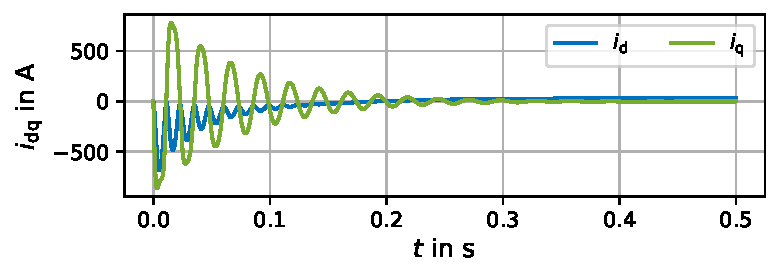
\includegraphics{ex06/i_dq_dampingW_ode.pdf}
        \caption{Transient process of a salient synchronous machine with a stator and field winding short circuit and a damper winding.}
        \label{fig:i_dq_dampingW_ode}
    \end{solutionfigure}

    The field current is visualized in \autoref{fig:i_f_dampingW_ode}.
    \begin{solutionfigure}[ht]
        \centering
        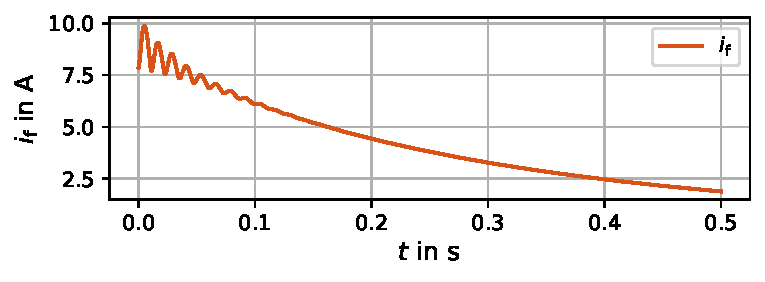
\includegraphics{ex06/i_f_dampingW_ode.pdf}
        \caption{Field current of a salient synchronous machine with a stator and field winding short circuit and a damper winding.}
        \label{fig:i_f_dampingW_ode}
    \end{solutionfigure}

    The rotational speed of the rotor is shown in \autoref{fig:omega_r_el_dampingW_ode}. The steady state is reached faster than in the simulation before, due to the added damping winding.
    \begin{solutionfigure}[ht]
        \centering
        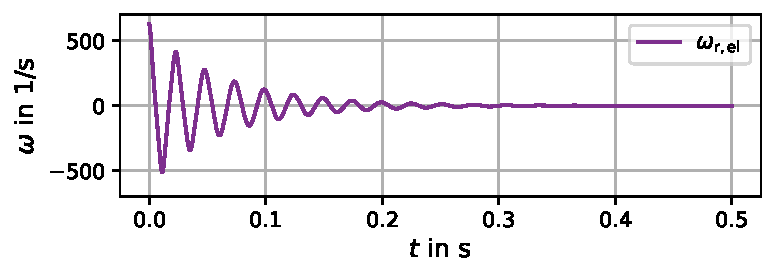
\includegraphics{ex06/omega_r_el_dampingW_ode.pdf}
        \caption{Speed of a salient synchronous machine with a stator and field winding short circuit and a damper winding.}
        \label{fig:omega_r_el_dampingW_ode}
    \end{solutionfigure}

    \autoref{fig:T_dampingW_ode} shows the generated torque during the transient process. The faster transient process is also visible in the torque curve, which faster converts to zero.
    \begin{solutionfigure}[ht]
        \centering
        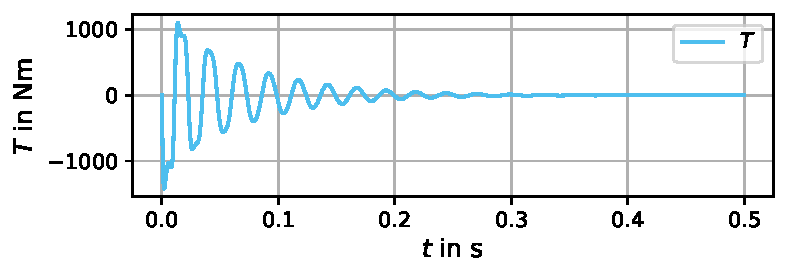
\includegraphics{ex06/T_dampingW_ode.pdf}
        \caption{Torque of a salient synchronous machine with a stator and field winding short circuit and a damper winding.}
        \label{fig:T_dampingW_ode}
    \end{solutionfigure}
\end{solutionblock}
\FloatBarrier

%%%%%%%%%%%%%%%%%%%%%%%%%%%%%%%%%%%%%%%%%%%%%%%%%%%%%%%%%%%%%
%% Task 2 %%
%%%%%%%%%%%%%%%%%%%%%%%%%%%%%%%%%%%%%%%%%%%%%%%%%%%%%%%%%%%%%

\task{Cylinderical synchronous machine}
In a thermal power station, a cylinderical synchronous generator is used which has the rated data in Tab.~\ref{tab:para_cylindericalSynchonousMachine} and is connected in star. The generator is driven by a turbine. The converted energy is fed into the 50 Hz national grid via a transformer. Saturation effects and losses in the machine can be neglected.
\begin{table}[htb]
    \caption{Parameters of the synchronous machine.}
    \centering
    \begin{tabular}{lll}\toprule
    Symbol  & Description       & Value \\
    \midrule
    $U_{\mathrm{star,n}}$ & Star voltage            & $\SI{\frac{10}{\sqrt{3}}}{\kilo\volt}$ \\
    $I_{\mathrm{star,n}}$ & Star current            & $\SI{6500}{\ampere}$ \\
    $f_{\mathrm{n}}$      & Nominal frequency       & $\SI{50}{\hertz}$ \\
    $\cos(\varphi_{\mathrm{n}})$    & Power factor  & 0.8 (capacitive) \\
    $n_{\mathrm{n}}$        & Nominal speed         & $\SI{1500}{\per\minute}$ \\
    $I_{\mathrm{f,n}}$    & Field current           & $\SI{150}{\ampere}$ \\ 
    $I_{\mathrm{s,sc0}}$  & Short circuit current   & $\SI{7800}{\ampere}$ \\
    \bottomrule
    \end{tabular}
    \label{tab:para_cylindericalSynchonousMachine}
\end{table}




%%%%%%%%%%%%%%%%%%%%%%%%%%%%%%%%%%%%%%%%%%%%%%%%%%%%%%%%%%%%%
\subtask{Synchronization must be carried out to connect the synchronous generator to the electricity grid. Why is this process necessary? Name the synchronization conditions that must be checked before the generator can be connected to the grid.}
\begin{solutionblock}
    Necessity of synchronization:
    \begin{itemize}
        \item Synchronization of the generator with the grid is absolutely essential for a complication-free connection of the machine to the grid. Otherwise, severe transient effects can lead to catastrophic effects.
        \item A high phase shift during the synchronization can start the machine to oscillate, but this is reduced by the damper winding in the rotor.
        \item In addition, connecting the generator with a large phase offset leads to high equalizing currents and thus a large torque are the result, which leads to the destruction of the generator.
    \end{itemize}

    Therefore, the following synchronization conditions should be fulfilled:
    \begin{itemize}
        \item The rotational frequency is equal to the grid frequency.
        \item The terminal voltage and the grid voltage are at the same level.
        \item The sense of rotation of the machine is equal to the grid.
        \item The phase orientation is equal to the grid.
    \end{itemize}

\end{solutionblock}




%%%%%%%%%%%%%%%%%%%%%%%%%%%%%%%%%%%%%%%%%%%%%%%%%%%%%%%%%%%%%
\subtask{How can the amount of active power output be influenced during generator operation? On the other hand, how can the inductive reactive power delivered or absorbed be influenced?}

\begin{solutionblock}
    The delivered active power can only be influenced by changing the mechanical input power. The delivered (over excitation) or absorbed (under excitation) reactive power is controlled via the field current.
\end{solutionblock}



%%%%%%%%%%%%%%%%%%%%%%%%%%%%%%%%%%%%%%%%%%%%%%%%%%%%%%%%%%%%%
\subtask{What is meant by synchronous condenser operation?}

\begin{solutionblock}
    In the synchronous condenser operation mode, only reactive power is delivered into or absorbed from the grid. The machine operates in no-load mode. This operation mode is used to control the reactive power within the grid. Sometimes, more or less reactive power is needed, dependant on the conditions of the considered time frame.
\end{solutionblock}

%%%%%%%%%%%%%%%%%%%%%%%%%%%%%%%%%%%%%%%%%%%%%%%%%%%%%%%%%%%%%
\subtask{Calculate with the given data the pole pair number $p$, the synchronous reactance $X_{\mathrm{s}}$, the apparent power $S$, the phase shift angle $\varphi$, the inner voltage $U_{\mathrm{i}}$ and the load angle $\theta$ at the rated conditions.}

\begin{solutionblock}
    The pole pair number is determined with:
    \begin{equation}
        p = \frac{\omega_{\mathrm{n}}}{\omega_{\mathrm{mech}}}
        = \frac{\SI{2\pi\cdot 50}{\per\second}}{\SI{2\pi \cdot 25}{\per\second}}
        = 2.
    \end{equation}

    The synchronous reactance is calculated by
    \begin{equation}
        X_{\mathrm{s}} = \frac{U_{\mathrm{s}}}{I_{\mathrm{s,sc0}}}
        = \frac{\SI{\frac{10000}{\sqrt{3}}}{\volt}}{\SI{7800}{\ampere}}
        = \SI{0.74}{\Omega},
    \end{equation}
    with the stator voltage $U_{\mathrm{s}}$ and the short circuit current $I_{\mathrm{s,sc0}}$.
    The apparent power determines as
    \begin{equation}
        S = \sqrt{3} U_{\mathrm{n}} I_{\mathrm{n}}
        = \sqrt{3}\cdot \SI{10000}{\volt}\cdot\SI{6500}{\ampere}
        = \SI{112.58}{\mega\volt\ampere},
    \end{equation}
    and this leads to the calculation of the phase shift angle by:
    \begin{equation}
        \varphi = \arccos(-0.8)\cdot \mathrm{sign}\left(\frac{Q}{S}\right)
        = - \arccos(-0.8) = \SI{-143.13}{\degree}.
    \end{equation}

    The inner voltage is calculated with
    \begin{equation}
        U_{\mathrm{i}} = X_{\mathrm{s}} I_{\mathrm{s,sc}}
        = X_{\mathrm{s}} \left(\frac{I_{\mathrm{s,sc0}}-I_{\mathrm{s}}\sin(\varphi)}{\cos(\varphi)}\right),
    \end{equation}
    and the active power is defined as:
    \begin{equation}
        P = \frac{3 U_{\mathrm{s}}U_{\mathrm{i}}}{X_{\mathrm{s}}} \sin(\theta).
    \end{equation}
    Inserting the inner voltage from above into the active power equation, yields:
    \begin{equation}
        P = \frac{3 U_{\mathrm{s}} X_{\mathrm{s}} \left(\frac{I_{\mathrm{s,sc0}}-I_{\mathrm{s}}\sin(\varphi)}{\cos(\varphi)}\right)}{X_{\mathrm{s}}} \sin(\theta)
        = 3 U_{\mathrm{s}} \left(I_{\mathrm{s,sc0}}-I_{\mathrm{s}} \sin(\varphi)\right) \tan(\theta).
    \end{equation}

    Hence, the load angle is determined with resorting the equation from above as follows:
    \begin{align}
        \begin{split}
        \theta &= \arctan\left(\frac{P}{3 U_{\mathrm{s}}(I_{\mathrm{s,sc0}}-I_{\mathrm{s,sc}}\sin(\varphi))}\right)
        =\arctan\left(\frac{3 U_{\mathrm{s}} I_{\mathrm{s}} \cos(\varphi)}{3 U_{\mathrm{s}}(I_{\mathrm{s,sc0}}-I_{\mathrm{s,sc}}\sin(\varphi))}\right) \\
        &= \arctan\left(\frac{I_{\mathrm{s}}\cos(\varphi)}{I_{\mathrm{s,sc0}}-I_{\mathrm{s}}\sin(\varphi)} \right)
        = \arctan\left(\frac{\SI{6.5}{\kilo\ampere}\cdot \cos(\SI{-143.13}{\degree})}{\SI{7.8}{\kilo\ampere}-\SI{6.5}{\kilo\ampere}\cdot\sin(\SI{-143.13}{\degree})}\right)
        = \SI{-23.95}{\degree}.
        \end{split}
        \label{eq:load_angle}
    \end{align}

    The inner voltage is calculated by:
    \begin{equation}
        U_{\mathrm{i}} = X_{\mathrm{s}} I_{\mathrm{s,sc}}
        = X_{\mathrm{s}} \left(\frac{I_{\mathrm{s,sc0}}- I_{\mathrm{s}}\sin(\varphi)}{\cos(\theta)}\right)
        = \SI{0.74}{\Omega}\cdot\left(\frac{\SI{7.8}{\kilo\ampere}-\SI{6.5}{\kilo\ampere}\cdot\sin(\SI{-143.13}{\degree})}{\cos(\SI{-23.95}{\degree})}\right)
        = \SI{9473}{\volt}.
    \end{equation}
\end{solutionblock}


%%%%%%%%%%%%%%%%%%%%%%%%%%%%%%%%%%%%%%%%%%%%%%%%%%%%%%%%%%%%%
\subtask{The generator should only take reactive power from the grid. How large is the stator current $I_{\mathrm{s}}$ and the field current $I_{\mathrm{f}}$ at this operating point, when a reactive power of 120 MVA is extracted from the grid? How large is the phase shift angle $\varphi$ and the load angle $\theta$? Draw the phasor diagram for this operating point.}

\begin{solutionblock}
    The stator current changes to
    \begin{equation}
        I_{\mathrm{s}} = \frac{Q}{\sqrt{3}U_{\mathrm{n}}\sin(\varphi)}
        = \frac{\SI{120}{\mega\volt\ampere}}{\SI{\sqrt{3}\cdot10}{\kilo\volt}}
        = \SI{6928.2}{\ampere},
    \end{equation}

    and the inner voltage is determined with:
    \begin{equation}
        U_{\mathrm{i}} = \frac{3 U_{\mathrm{s}}^2 - X_{\mathrm{s}}Q}{3U_{\mathrm{s}}\cos(\theta)}
        = \frac{3\cdot\left(\frac{\SI{10}{\kilo\volt}}{\sqrt{3}}\right)^2 - \SI{0.74}{\Omega}\cdot\SI{120}{\mega\volt\ampere}}{3\cdot\frac{\SI{10}{\kilo\volt}}{\sqrt{3}}\cos(\SI{0}{\degree})}
        = \SI{1501.11}{\volt}.
    \end{equation}

    Therefore, the necessary field current results in
    \begin{equation}
        I_{\mathrm{f}} = \frac{U_{\mathrm{i}}}{U_{\mathrm{i,n}}}I_{\mathrm{f,n}}
        = \frac{\SI{1501.11}{\volt}}{\SI{9473}{\volt}}\cdot \SI{150}{\ampere}
        = \SI{23.77}{\ampere}.
    \end{equation}

    The phase shift angle is $\varphi = \SI{90}{\degree}$ and the load angle is $\theta = \SI{0}{\degree}$. The phasor diagram is visualized in \autoref{fig:Phasor_diagram_reactive}, the inner voltage $\underline{U}_{\mathrm{i}}$ is purely imaginary, as defined in the lecture notes. The stator voltage $\underline{U}_{\mathrm{s}}$ and the internal voltage are directly on top of each other due to the zero load angle $\theta$.
    \begin{solutionfigure}[ht]
        \centering
        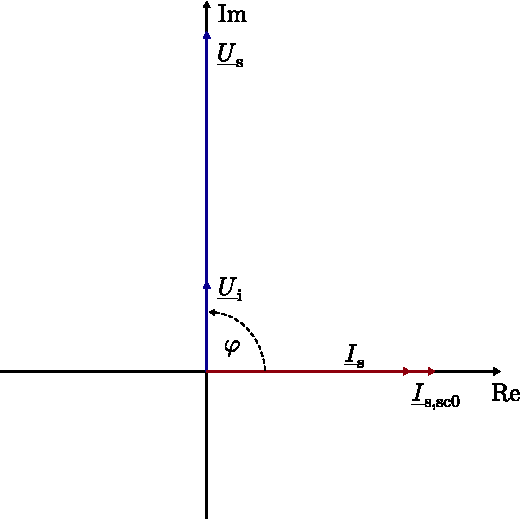
\includegraphics{ex06/Phasor_diagram_reactive.pdf}
        \caption{Phasor diagram for the given operating point. The scala is for the voltage 1 cm $\widehat{=}~ \SI{1000}{\volt}$ and for the current 1 cm $\widehat{=}~ \SI{2000}{\ampere}$.}
        \label{fig:Phasor_diagram_reactive}
    \end{solutionfigure}

\end{solutionblock}


%%%%%%%%%%%%%%%%%%%%%%%%%%%%%%%%%%%%%%%%%%%%%%%%%%%%%%%%%%%%%
\subtask{In contrast to the previous subtask, the generator should provide 80 MW in addition to the reactive power now. How large is the stator current $I_{\mathrm{s}}$, the phase shift angle $\varphi$ and the load angle $\theta$? Draw also for this operation point the phasor diagram.}

\begin{solutionblock}
    
    The apparent power is:
    \begin{equation}
        S = \sqrt{P^2+Q^2}
        = \sqrt{\left(\SI{80}{\mega\watt}\right)^2 + \left(\SI{120}{\mega\volt\ampere}\right)^2}
        = \SI{144.22}{\mega\volt\ampere}.
    \end{equation}

    Hence, the stator current yields:
    \begin{equation}
        I_{\mathrm{s}} = \frac{S}{\sqrt{3}U_{\mathrm{n}}}
        = \frac{\SI{144.22}{\mega\volt\ampere}}{\sqrt{3}\cdot\SI{10}{\kilo\volt}}
        = \SI{8326.54}{\ampere}.
    \end{equation}

    Retrieving the power factor via the complex power equation leads to:
    \begin{equation}
        \varphi = \arccos\left(\frac{-P}{\sqrt{3}U_{\mathrm{s,n}}I_{\mathrm{s}}} \right)
        = \arccos\left(\frac{-\SI{80}{\mega\watt}}{\sqrt{3}\cdot\SI{10}{\kilo\volt}\cdot\SI{8326.54}{\ampere}}\right)
        = \SI{123.7}{\degree}.
    \end{equation}

    The derivation of the load angle is already given in \eqref{eq:load_angle}, which results for the new operation point in
    \begin{equation}
        \theta = \arctan\left(\frac{I_{\mathrm{s}}\cos(\varphi)}{I_{\mathrm{s,sc0}}-I_{\mathrm{s}}\sin(\varphi)}\right)
        = \SI{-79.66}{\degree},
    \end{equation}
    while the resulting inner voltage is
    \begin{equation}
        U_{\mathrm{i}} = X_{\mathrm{s}} I_{\mathrm{s,sc}}
        = \SI{3600}{\volt}.
    \end{equation}

    The phasor diagram is visualized in \autoref{fig:Phasor_diagram_reactive_active}, the inner voltage $\underline{U}_{\mathrm{i}}$ is purely imaginary, as defined in the lecture notes.
    \begin{solutionfigure}
        \centering
        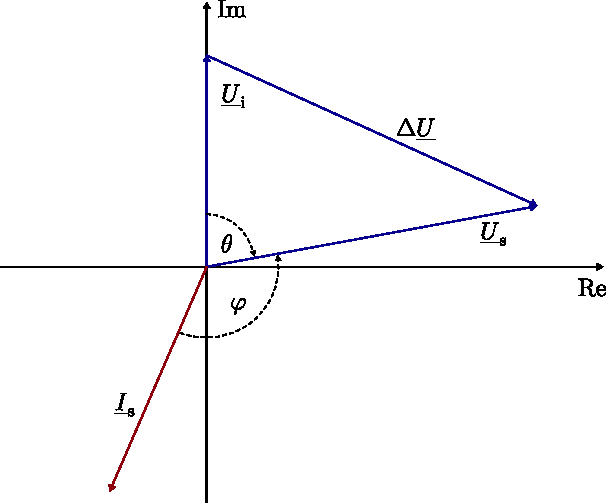
\includegraphics{ex06/Phasor_diagram_reactive_active.pdf}
        \caption{Phasor diagram for the given operating point. The scala is for the voltage 1 cm $\widehat{=}~ \SI{1000}{\volt}$ and for the current 1 cm $\widehat{=}~ \SI{2000}{\ampere}$.}
        \label{fig:Phasor_diagram_reactive_active}
    \end{solutionfigure}


\end{solutionblock}



%%%%%%%%%%%%%%%%%%%%%%%%%%%%%%%%%%%%%%%%%%%%%%%%%%%%%%%%%%%%%
\subtask{Now, the generator should provide a reactive power of 60 MVA into the grid. How large is the generated torque $T$, that the generator operates within the rated apparent power? To which value must the field current $I_{\mathrm{f}}$ change, such that the rated current is reached in the stator winding?}

\begin{solutionblock}
    With the determined rated apparent power in the task before, the given reactive power, the maximum power is calculated by
    \begin{equation}
        P = \sqrt{S_{\mathrm{n}}^2 - Q^2}
        = \sqrt{\left(\SI{112.58}{\mega\volt\ampere}\right)^2 - \left(\SI{60}{\mega\volt\ampere}\right)^2}
        = \SI{95.26}{\mega\watt},
    \end{equation}
    hence, the maximum torque is given with:
    \begin{equation}
        T_{\mathrm{max}} = \frac{P}{\omega_{\mathrm{mech,n}}}
        = \frac{\SI{95.26}{\mega\watt}}{\SI{2\pi\cdot 25}{\per\second}}
        = \SI{606.5}{\kilo\newton\metre}.
    \end{equation}
    

    The angle $\varphi$ for the phase shift at nominal current is determined as:
    \begin{equation}
        \varphi = \arccos\left(\frac{P}{\sqrt{3}U_{\mathrm{star,n} I_{\mathrm{star,n}}}}\right)
        = \arccos\left(\frac{-\SI{95.26}{\mega\watt}}{\sqrt{3}\cdot \SI{10}{\kilo\volt}\cdot \SI{6.5}{\kilo\ampere}}\right)
        = -\SI{147.8}{\degree}.
    \end{equation}

    With \eqref{eq:load_angle} the load angle is calculated by
    \begin{equation}
        \theta = \arccos\left(\frac{I_{\mathrm{s}}\cos(\varphi)}{I_{\mathrm{s,sc0}}-I_{\mathrm{s,sc}}\sin(\varphi)}\right)
        = \arctan\left(\frac{\SI{6.5}{\kilo\ampere}\cos(\SI{-147.8}{\degree})}{\SI{7.8}{\kilo\ampere}-\SI{6.5}{\kilo\ampere}\sin(\SI{-147.8}{\degree})}\right)
        = \SI{-26.03}{\degree},
    \end{equation}
    therefore, the inner voltage results into:
    \begin{equation}
        U_{\mathrm{i}} = X_{\mathrm{s}} I_{\mathrm{s,sc}}
        = X_{\mathrm{s}} \left(\frac{I_{\mathrm{s,sc0}}-I_{\mathrm{s}}\sin(\varphi)}{\cos(\theta)}\right)
        = \SI{0.74}{\Omega}\left(\frac{\SI{7.8}{\kilo\ampere}-\SI{6.5}{\kilo\ampere}\sin(\SI{-147.8}{\degree})}{\cos(\SI{-26.03}{\degree})}\right)
        = \SI{9276}{\volt}.
    \end{equation}

    The field current must be set to the following value:
    \begin{equation}
        I_{\mathrm{f}} = \frac{U_{\mathrm{i}}}{U_{\mathrm{i,n}}}I_{\mathrm{f,n}}
        = \frac{\SI{9276}{\volt}}{\SI{9473}{\volt}}\cdot \SI{150}{\ampere}
        = \SI{146.9}{\ampere}.
    \end{equation}

\end{solutionblock}

\FloatBarrier


%%%%%%%%%%%%%%%%%%%%%%%%%%%%%%%%%%%%%%%%%%%%%%%%%%%%%%%%%%%%%
%% Task 3 %%
%%%%%%%%%%%%%%%%%%%%%%%%%%%%%%%%%%%%%%%%%%%%%%%%%%%%%%%%%%%%%

\task{Steady-state operation of a synchronous machine}
Consider a loss-free synchronous machine with the parameters from Tab.~\ref{tab:para_SynchonousMachine}. First, the synchronous machine is operated as a a motor. Using the data given above, determine the following characteristic variables of the synchronous machine at rated operation. An example phasor diagram for this operation is shown in \autoref{fig:Phasor_diagrams_m_oe}.


\begin{table}[htb]
    \caption{Parameters of the synchronous machine.}
    \centering
    \begin{tabular}{lll}\toprule
    Symbol  & Description       & Value \\
    \midrule
    $U_{\mathrm{star,n}}$ & Star voltage            & $\SI{\frac{6}{\sqrt{3}}}{\kilo\volt}$ \\
    $I_{\mathrm{star,n}}$ & Star current            & $\SI{96}{\ampere}$ \\
    $f_{\mathrm{n}}$      & Nominal frequency       & $\SI{50}{\hertz}$ \\
    $p$                   & Pole pair number        & 2 \\
    $\cos(\varphi_{\mathrm{n}})$    & Power factor  & 0.9 (capacitive) \\
    $T_{\mathrm{n}}$      & Nominal torque          & $\frac{T_{\mathrm{max}}}{2}$ \\
    \bottomrule
    \end{tabular}
    \label{tab:para_SynchonousMachine}
\end{table}

\begin{figure}[ht]
    \centering
    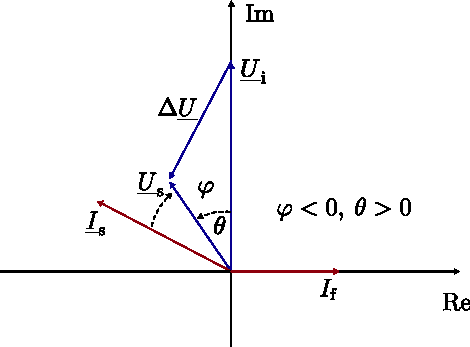
\includegraphics{ex06/Phasor_diagrams_m_oe.pdf}
    \caption{Phasor diagram of a over excited synchronous machine in motor mode.}
    \label{fig:Phasor_diagrams_m_oe}
\end{figure}

%%%%%%%%%%%%%%%%%%%%%%%%%%%%%%%%%%%%%%%%%%%%%%%%%%%%%%%%%%%%%
\subtask{How large is the maximum torque $T_{\mathrm{max}}$?}

\begin{solutionblock}

    Due to the ideal machine characteristic (no losses), the nominal torque is calculated by
    \begin{equation}
        T_{\mathrm{n}} = \frac{P_{\mathrm{n}}}{\omega_{\mathrm{mech,n}}}
        = \frac{3 U_{\mathrm{star,n}} I_{\mathrm{star,n}} \cos(\varphi)}{\omega_{\mathrm{mech,n}}}
        = \frac{\sqrt{3}\cdot \SI{6000}{\volt}\cdot\SI{96}{\ampere}\cdot0.9}{\SI{2\pi\cdot50}{\per\second}}
        = \SI{2858}{\newton\metre},
    \end{equation}

    and, the maximum torque calculates as follows:
    \begin{equation}
        T_{\mathrm{max}} = 2 T_{\mathrm{n}}
        = 2 \cdot \SI{2858}{\newton\metre}
        = \SI{5716}{\newton\metre}.
    \end{equation}
    
\end{solutionblock}



%%%%%%%%%%%%%%%%%%%%%%%%%%%%%%%%%%%%%%%%%%%%%%%%%%%%%%%%%%%%%
\subtask{Which load angle $\theta$ is set at the nominal operating point?}

\begin{solutionblock}
    The load angle can be determined by geometric transformations, which are shown in \autoref{fig:syn_motor_overExcited}.
    \begin{solutionfigure}
        \centering
        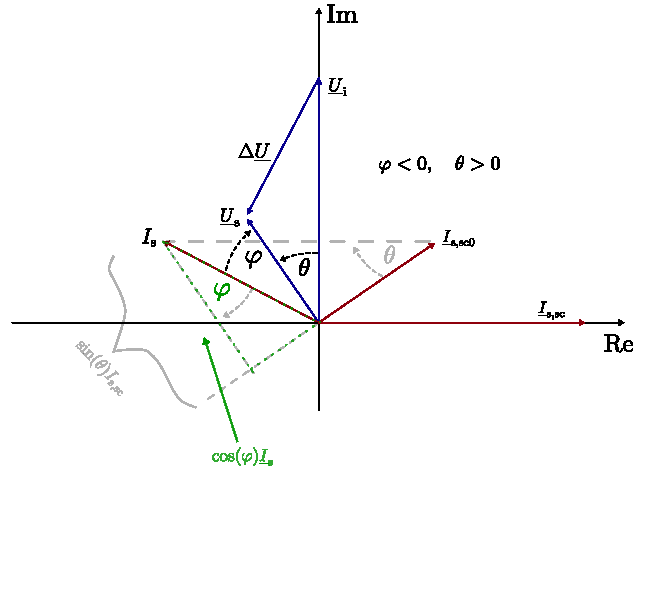
\includegraphics{ex06/syn_motor_overExcited.pdf}
        \caption{Phasor diagram for an over excited synchronous machine in motor operation.}
        \label{fig:syn_motor_overExcited}
    \end{solutionfigure}
    
    The target is to create two different triangles, one with the known angle $\varphi$ (marked in green in the figure) and one without the load angle $\theta$ (marked in gray in the figure). 
    Hence, the load angle calculates as follows
    \begin{align}
        \begin{split}
            \sin(\theta) I_{\mathrm{s,sc}} = \cos(\varphi)I_{\mathrm{s}},\\
            \sin(\theta) = \frac{I_{\mathrm{s}}}{I_{\mathrm{s,sc}}}\cos(\varphi),
        \end{split}
    \end{align}
    which leads to the angle:
    \begin{equation}
        \theta = \arcsin\left(\frac{I_{\mathrm{s}}}{I_{\mathrm{s,sc}}} \right) \cos(\varphi)
        = \arcsin\left(\frac{\SI{96}{\ampere}}{\SI{172.8}{\ampere}}\right) \cdot 0.9
        = \SI{30}{\degree}.
    \end{equation}
\end{solutionblock}

%%%%%%%%%%%%%%%%%%%%%%%%%%%%%%%%%%%%%%%%%%%%%%%%%%%%%%%%%%%%%
\subtask{Determine the synchronous reactance $X_{\mathrm{s}}$ value.}

\begin{solutionblock}
    The reactance is determined as:
    \begin{align}
        \begin{split}
        X_{\mathrm{s}}
        &= \frac{U_{\mathrm{i}}}{I_{\mathrm{s,sc}}}
        = \frac{U_{\mathrm{s}}}{I_{\mathrm{s,sc0}}}
        = \frac{U_{\mathrm{s}}}{I_{\mathrm{s}}\sin(\arccos(0.9)\mathrm{sign}(Q/S))+I_{\mathrm{s,sc}}\cos(\theta)} \\
        &= \frac{\SI{\frac{6000}{\sqrt{3}}}{\volt}}{\SI{96}{\ampere}\cdot \sin(\SI{-25.8}{\degree}) + \SI{172.8}{\ampere}\cdot \cos(\SI{30}{\degree})}
        = \SI{32.12}{\Omega}.
        \end{split}
    \end{align}

\end{solutionblock}


%%%%%%%%%%%%%%%%%%%%%%%%%%%%%%%%%%%%%%%%%%%%%%%%%%%%%%%%%%%%%
\subtask{Calculate the inner voltage $U_{\mathrm{i}}$ at the nominal operating point.}
\begin{solutionblock}
    
    \begin{equation}
        U_{\mathrm{i}} = X_{\mathrm{s}} I_{\mathrm{s,sc}}
        = \SI{32.12}{\Omega} \cdot \SI{172.79}{\ampere}
        = \SI{5549.52}{\volt}
    \end{equation}
\end{solutionblock}




%%%%%%%%%%%%%%%%%%%%%%%%%%%%%%%%%%%%%%%%%%%%%%%%%%%%%%%%%%%%%
\subtask{In the next task, the machine operates as generator and the power is 500 kW. The phasor diagram for this operation is shown in \autoref{fig:Phasor_diagrams_gen_oe}. Which load angle $\theta$ is set at the new operating point?}

\begin{figure}[ht]
    \centering
    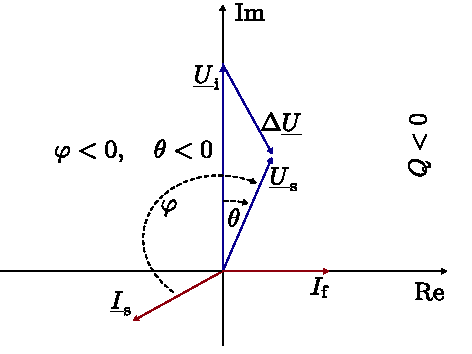
\includegraphics{ex06/Phasor_diagrams_gen_oe.pdf}
    \caption{Phasor diagram of an over excited synchronous machine in generator mode.}
    \label{fig:Phasor_diagrams_gen_oe}
\end{figure}


\begin{solutionblock}
    In the generator mode, the load angle is negative. With the generated power of 500 kW and the constant voltage, the product of the current and power factor is determined by:
    \begin{equation}
        \cos(\varphi) I_{\mathrm{s}} = \frac{P}{3 U_{\mathrm{s}}}
        = \frac{\SI{-500}{\kilo\watt}}{3\cdot \SI{\frac{6000}{\sqrt{3}}}{\volt}}
        = -\SI{48.11}{\ampere}.
    \end{equation}

    It is also assumed that the short-circuit current has not changed its value by maintaining the excitation current. The load angle can now be determined using the trigonometric relationship:
    \begin{equation}
        \theta = \arcsin\left(\frac{I_{\mathrm{s}}}{I_{\mathrm{s,sc}}}\cos(\varphi)\right)
        = \arcsin\left(\frac{\SI{-48.11}{\ampere}}{\SI{172.8}{\ampere}}\right)
        = \SI{-16.17}{\degree}.
    \end{equation}
\end{solutionblock}


%%%%%%%%%%%%%%%%%%%%%%%%%%%%%%%%%%%%%%%%%%%%%%%%%%%%%%%%%%%%%
\subtask{Calculate the stator current $I_{\mathrm{s}}$.}

\begin{solutionblock}
    The stator current is calculated with the active and the reactive current components, which are defined as in the previous task by
    \begin{equation}
        I_{\mathrm{s}} = \sqrt{I_{\mathrm{active}}^2 + I_{\mathrm{reactive}}^2}
        = \sqrt{\left(I_{\mathrm{s}}\sin(-\varphi - \SI{90}{\degree})\right)^2 + \left(I_{\mathrm{s}}\cos(-\varphi - \SI{90}{\degree})\right)^2}.
    \end{equation}
    
    With the relationship between the trigonometric functions and the phase shift, the equation from above is resorted to:
    \begin{align}
        \begin{split}
            I_{\mathrm{s}} &= \sqrt{\left(-I_{\mathrm{s}}\cos(-\varphi)\right)^2 + \left(I_{\mathrm{s}}\sin(-\varphi)\right)^2} \\
            & = \sqrt{\left(-I_{\mathrm{s}}\cos(-\varphi)\right)^2 + \left(-I_{\mathrm{s}}\sin(\varphi)\right)^2}.
        \end{split}
    \end{align}

    With the triangular relationship:
    \begin{align}
        \begin{split}
        I_{\mathrm{s}} &= \sqrt{\left(-I_{\mathrm{s}}\cos(-\varphi)\right)^2 + \left(I_{\mathrm{s,sc0}}-I_{\mathrm{s,sc}}\cos(\theta)\right)^2} \\
        &= \sqrt{\left(-I_{\mathrm{s}}\cos(-\varphi)\right)^2 + \left(I_{\mathrm{s,sc0}}+I_{\mathrm{s,sc}}\cos(\theta)\right)^2}.
        \end{split}
    \end{align}

    Use the calculation of the short circuit current $I_{\mathrm{s,sc0}}$, leads to:
    \begin{align}
        \begin{split}
            I_{\mathrm{s}} &= \sqrt{\left(-I_{\mathrm{s}}\cos(-\varphi)\right)^2 + \left(-\frac{U_{\mathrm{s}}}{X_{\mathrm{s}}}+I_{\mathrm{s,sc}}\cos(\theta)\right)^2} \\
            &= \sqrt{\left(\SI{48.11}{\ampere}\right)^2 + \left(-\frac{\SI{\frac{6000}{\sqrt{3}}}{\volt}}{\SI{32.12}{\Omega}} + \SI{172.79}{\ampere}\cos(-\SI{16.17}{\degree})\right)^2} \\
            &= \SI{75.44}{\ampere}.
        \end{split}
    \end{align}

\end{solutionblock}


%%%%%%%%%%%%%%%%%%%%%%%%%%%%%%%%%%%%%%%%%%%%%%%%%%%%%%%%%%%%%
\subtask{How large is the power factor $\cos(\varphi)$ at this operating point? In addition, calculate the angle $\varphi$.}

\begin{solutionblock}
    The active power is calculated with
    \begin{equation}
        I_{\mathrm{active}} = I_{\mathrm{s}} \cos(\varphi),
    \end{equation}
    which than leads to
    \begin{equation}
        \cos(\varphi) = \frac{I_{\mathrm{active}}}{I_{\mathrm{s}}} 
        = \frac{I_{\mathrm{s}}\cos(\varphi)}{I_{\mathrm{s}}}
        = \frac{-\SI{48.11}{\ampere}}{\SI{75.44}{\ampere}}
        = -0.638,
    \end{equation}
    and, therefore, the angle results into:
    \begin{equation}
        \varphi = \arccos(-0.638)\cdot \mathrm{sign}\left(\frac{Q}{S}\right)
        = -\arccos(-0.638) = \SI{-129.6}{\degree}.
    \end{equation}
\end{solutionblock}










\end{document}